% arara: xelatex
% arara: xelatex
% arara: xelatex


% options:
% thesis=B bachelor's thesis
% thesis=M master's thesis
% czech thesis in Czech language
% english thesis in English language
% hidelinks remove colour boxes around hyperlinks

\documentclass[thesis=M,english]{FITthesis}[2019/12/23]

%\usepackage[utf8]{inputenc} % LaTeX source encoded as UTF-8
% \usepackage[latin2]{inputenc} % LaTeX source encoded as ISO-8859-2
% \usepackage[cp1250]{inputenc} % LaTeX source encoded as Windows-1250

\usepackage{subfig} %subfigures
\let\subfigureautorefname=\figurename
\usepackage{minted}
\usepackage{listings} %code snippets
\usepackage{xcolor} %colors
\usepackage{colortbl}
\usepackage{amsmath}
\usepackage{makecell}
\renewcommand\cellalign{lc}
\usepackage{inconsolata}
\usepackage{verbatim}
\usepackage{xcolor}

% \usepackage{amsmath} %advanced maths
% \usepackage{amssymb} %additional math symbols

\usepackage{dirtree} %directory tree visualisation

% % list of acronyms
% \usepackage[acronym,nonumberlist,toc,numberedsection=autolabel]{glossaries}
% \iflanguage{czech}{\renewcommand*{\acronymname}{Seznam pou{\v z}it{\' y}ch zkratek}}{}
% \makeglossaries

\usemintedstyle{pastie}
% \usemintedstyle{bw}
\counterwithin{listing}{chapter}
\providecommand*{\listingautorefname}{Listing}
\definecolor{codebg}{rgb}{1, 1, 1}
\definecolor{codegreen}{rgb}{0, 0.53, 0}
\definecolor{codeblue}{rgb}{0, 0.2, 0.56}
\newcommand{\microcvar}{\textcolor{codegreen}{\textbf{var}}}
\newcommand{\microcoutput}{\textcolor{codeblue}{output}}
\newcommand{\microcalloc}{\textcolor{codeblue}{alloc}}
\newcommand{\microcnull}{\textcolor{codeblue}{null}}

\hypersetup{%
    pdfborder = {0 0 0}
}

% % % % % % % % % % % % % % % % % % % % % % % % % % % % % % 
% EDIT THIS
% % % % % % % % % % % % % % % % % % % % % % % % % % % % % % 

\department{Department of Theoretical Computer Science}
\title{Ahead-of-time compiler for the microC language}
\authorGN{Václav} %author's given name/names
\authorFN{Král} %author's surname
\author{Václav Král} %author's name without academic degrees
\authorWithDegrees{Bc. Václav Král} %author's name with academic degrees
\supervisor{doc. Ing. Filip Křikava, Ph.D.}
\acknowledgements{First, I would like to thank my supervisor doc. Ing. Filip Křikava, Ph.D. for all his advice and time he dedicated to helping me with this thesis. I would also like to thank my friends and family who helped me a lot during my studies and provided the much needed psychological support.}

\abstractEN{The aim of this thesis is to implement an ahead-of-time optimizing compiler for \emph{microC}---language used in the NI-APR (Selected Methods for Program Analysis) course at FIT CTU for teaching program analyses. The compiler should primarily serve as an educational material of the course NI-APR, which demonstrates application and usefulness of selected static analyses during compilation and optimization. In this thesis, the reader will get familiar with not only the architecture of compilers, but also with the static analyses supported by the compiler. Further in this thesis, the design and most importantly the implementation are discussed. The optimization capabilities of the implementation are then demonstrated on several examples. Some of the possible future work improvements are proposed at the end of the thesis. The result of the thesis is a working optimizing microC compiler.}

\abstractCS{Cílem této práce je implementace ahead-of-time optimalizujícího kompilátoru \emph{microC}---jazyku, který se používá v předmětu NI-APR (Vybrané metody analýzy programů) na FIT ČVUT pro výuku analýz programů. Tento kompilátor má především sloužit jako učební pomůcka předmětu NI-APR, která demonstruje uplatnění a užitečnost vybraných statických analýz při kompilaci a optimalizaci. V práci se čtenář seznámí nejen s architekturou kompilátorů, ale i s jednotlivými statickými analýzami, které kompilátor podporuje. Dále se práce zabývá návrhem a především implementací kompilátoru. Optimalizační schopnosti implementace jsou poté demonstrovány na několika ukázkových příkladech. Závěrem práce navrhuje možná zlepšení a rozšíření. Výsledkem práce je funkční optimalizující kompilátor jazyku microC.}
\placeForDeclarationOfAuthenticity{Prague}
\keywordsCS{kompilátor, optimalizace, statická analýza kódu, microC, x86, Scala}
\keywordsEN{compiler, optimization, static program analysis, microC, x86, Scala}
\declarationOfAuthenticityOption{1} %select as appropriate, according to the desired license (integer 1-6)
% \website{http://site.example/thesis} %optional thesis URL


\begin{document}

% \newacronym{CVUT}{{\v C}VUT}{{\v C}esk{\' e} vysok{\' e} u{\v c}en{\' i} technick{\' e} v Praze}
% \newacronym{FIT}{FIT}{Fakulta informa{\v c}n{\' i}ch technologi{\' i}}

\setsecnumdepth{part}
\chapter{Introduction}
A typical program written by humans often contains many redundant operations \cite[Chap. 9.1.1]{dragonbook}. The origin of these redundancies may differ; some of them are available at the source level\footnote{E.g., a programmer may find it more convenient to recalculate some result instead of reusing the already calculated value.} and some of them are the consequence of writing the program in a high-level language. The task of an optimizing compiler is to transform these redundancies, as well as many other imperfections in a program, in a way that will improve\footnote{Note that the \emph{improvement} does not necessarily mean a faster execution of the compiled program \cite[Chap. 8.1]{eng_comp}. It can also mean smaller code size (which does not automatically imply a faster execution) or lesser memory footprint of the running program.} the quality of the program---such transformation is called an \emph{optimization}. However, in order for the compiler to be able to perform these optimizations, it needs to know various properties of the program, such as \cite[Chap 1.1]{spa}:
\begin{itemize}
    \item Has the value of an expression already been calculated?
    \item Is the program statement unreachable for every possible program input?
    \item Does the value of some variable depend on the program input, or is it always the same value?
\end{itemize}

To answer such questions, the compiler utilizes \emph{static program analyses}, which aim to give information about the possible behaviours of the program without actually running it \cite[Introduction]{spa}. However, as stated in Rice's theorem~\cite{rice}, these questions are \emph{undecidable} for Turing-complete languages and therefore the answers given by the analyses generally must involve \emph{approximation}. Depending on the type of approximation, we can divide these analyses into two types \cite[Chap. 5.8]{spa}:
\pagebreak
\begin{itemize}
    \item \emph{May analyses}, which give guarantees about what programs \emph{may} do, therefore computing an \emph{over}-approximation. An example of such analysis is the \emph{live variable analysis}, which gives information about what variables \emph{may} be read (i.e., are live) during the program execution.
    \item \emph{Must analyses}, which describe information about programs that \emph{must} definitely be true, therefore computing an \emph{under}-approximation. An example of such analysis is the \emph{available expression analysis}, which gives information about what expressions \emph{must} have been already computed earlier (i.e., are available) in the program execution.
\end{itemize}

While the analyses give only approximative guarantees about the programs, they are still very useful not only for the optimization as we already stated (which was the original purpose of the static program analyses), but also, e.g., for finding bugs in programs.

At FIT CTU, the NI-APR course (Selected Methods for Program Analysis)~\cite{apr} focuses on some of the most classical program analyses. In the first half of the course, students are implementing static analyses of programs written in \emph{microC}---a tiny C-like programming language, yet with some interesting features such as pointers, records, or function values. The problem is that students only implement the analyses and do not see their effects on programs that could have been done by an optimizing compiler. Therefore, the goal of this work is to fill this gap and create an optimizing compiler for microC. The compiler will use the analyses developed by the NI-APR students and produce optimized x86-64 assembly. It should serve as an educational material that helps students to understand the usefulness and importance of the analyses taught in the NI-APR course. With the compiler, students will be able to closely observe the effects of static analyses on the compilation and compare the changes and improvements in the programs produced by the compiler. The main emphasis in the implementation is on compatibility with the course codebase written in Scala and since the compiler will be used as an educational material, the implementation should also be easy to follow (clarity is preferred over conciseness), documented, and well tested.

The thesis is structured into four chapters. We open the background chapter with a brief overview of compiler design, followed by an introduction of the microC language, the x86-64 assembly, and static analyses used by the compiler. In the design chapter, we discuss the design of each part of the compiler. Then, in the implementation chapter, we go over implementation, testing, and documentation of the compiler. Lastly, in the assessment chapter, we demonstrate the optimization capabilities of the compiler.

\setsecnumdepth{all}



\chapter{Background}
We open this chapter with a brief introduction to compiler design. Then we introduce both source and target languages of our compiler. In the last section of this chapter, we provide a brief overview of static program analyses we will be utilizing in our compiler.

\section{Compiler}
Most programming languages are designed to be a human-readable way to express all sorts of computations as a sequence of operations. These operations are then expected to be executed on computer processors. However, the machine operations that a processor implements are often at a much lower-level of abstraction than those defined in a programming language \cite[Chap. 1.1]{eng_comp}. That's why every programming language operation has to be translated into (often a large number of) machine operations before it can be executed.

The tool that performs these translations is called a \emph{compiler}. Simply put, a compiler is a program that reads a program in one language (called \emph{source language}) and translates it into an equivalent program in another language\footnote{Note that the language may not necessarily be a machine code---some compilers produce a program written in another human-readable programming language.} (called \emph{target language}) \cite[Chap. 1.1]{dragonbook}. This process is shown in \autoref{fig:compiler}.

\begin{figure}
    \centering
    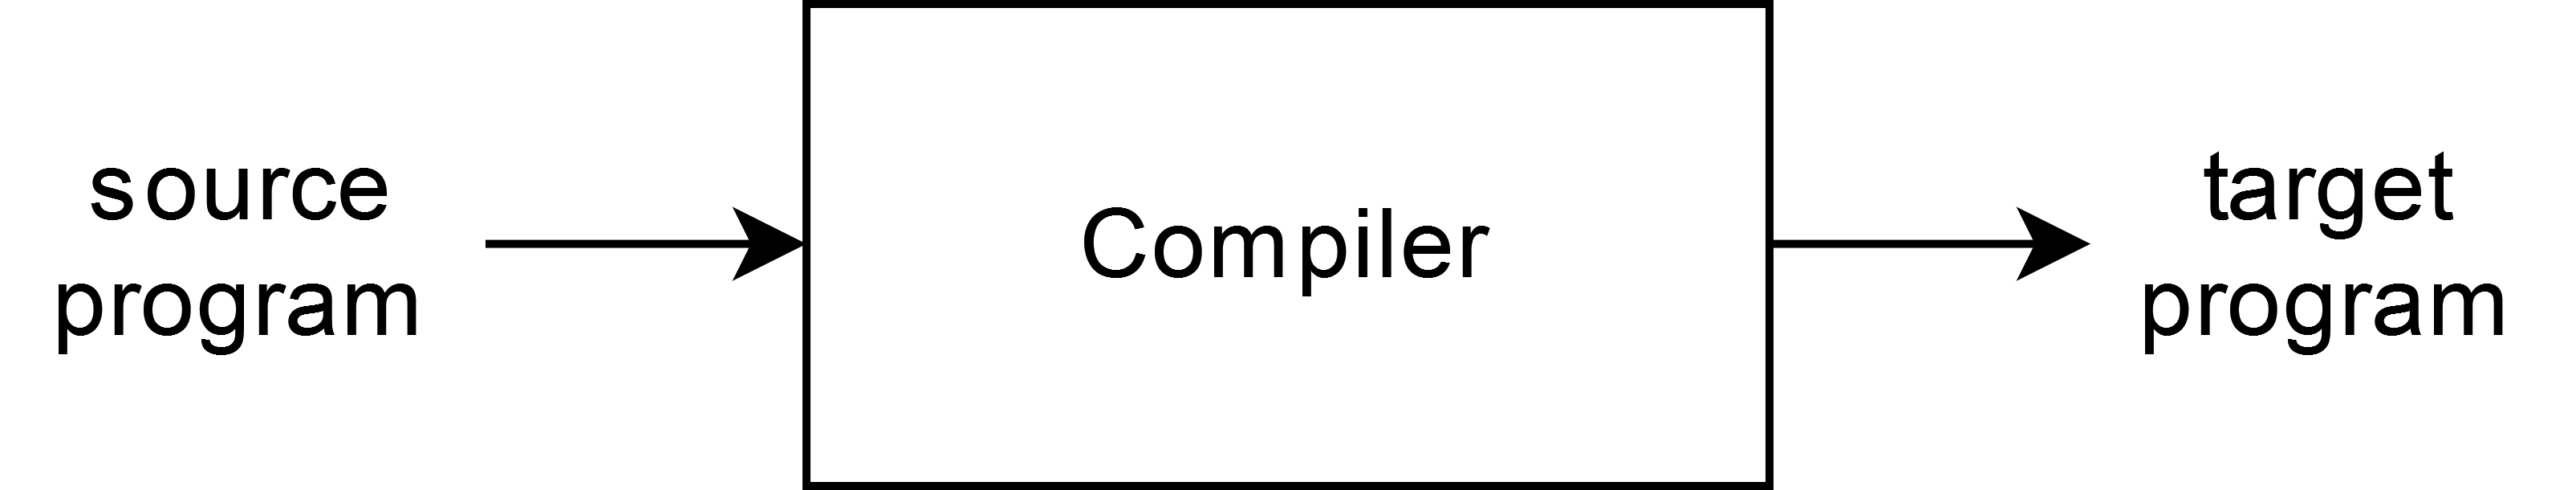
\includegraphics[width=9cm]{img/compiler.png}
    \caption{A compiler.}\label{fig:compiler}
\end{figure}

\pagebreak

There are many types of compilers and compilation strategies. In this thesis, we focus on a classical \emph{ahead-of-time} (AOT) compiler that compiles a high-level programming language into a lower-level one before execution rather than during the execution. Concretely, a compiler that compiles microC source code into Linux native x86-64 assembly. We will properly introduce both of these languages later in this chapter.

\subsection{Modularization}\label{ssec:modularization}
The \autoref{fig:compiler} depicts the compiler as a some kind of “black box” that takes the source program and produces the target program. This could incorrectly imply that the compiler takes the source language and maps its functionality directly to the target language, which is often not the case. In reality, the compiler is often decoupled into three smaller “boxes” (as shown in \autoref{fig:three_stage_compiler}) which represent three stages of a compilation:

\begin{itemize}
    \item \emph{Frontend} (or \emph{front end})
    \item \emph{Middleend} (or \emph{middle end})
    \item \emph{Backend} (or \emph{back end})
\end{itemize}

\begin{figure}
    \centering
    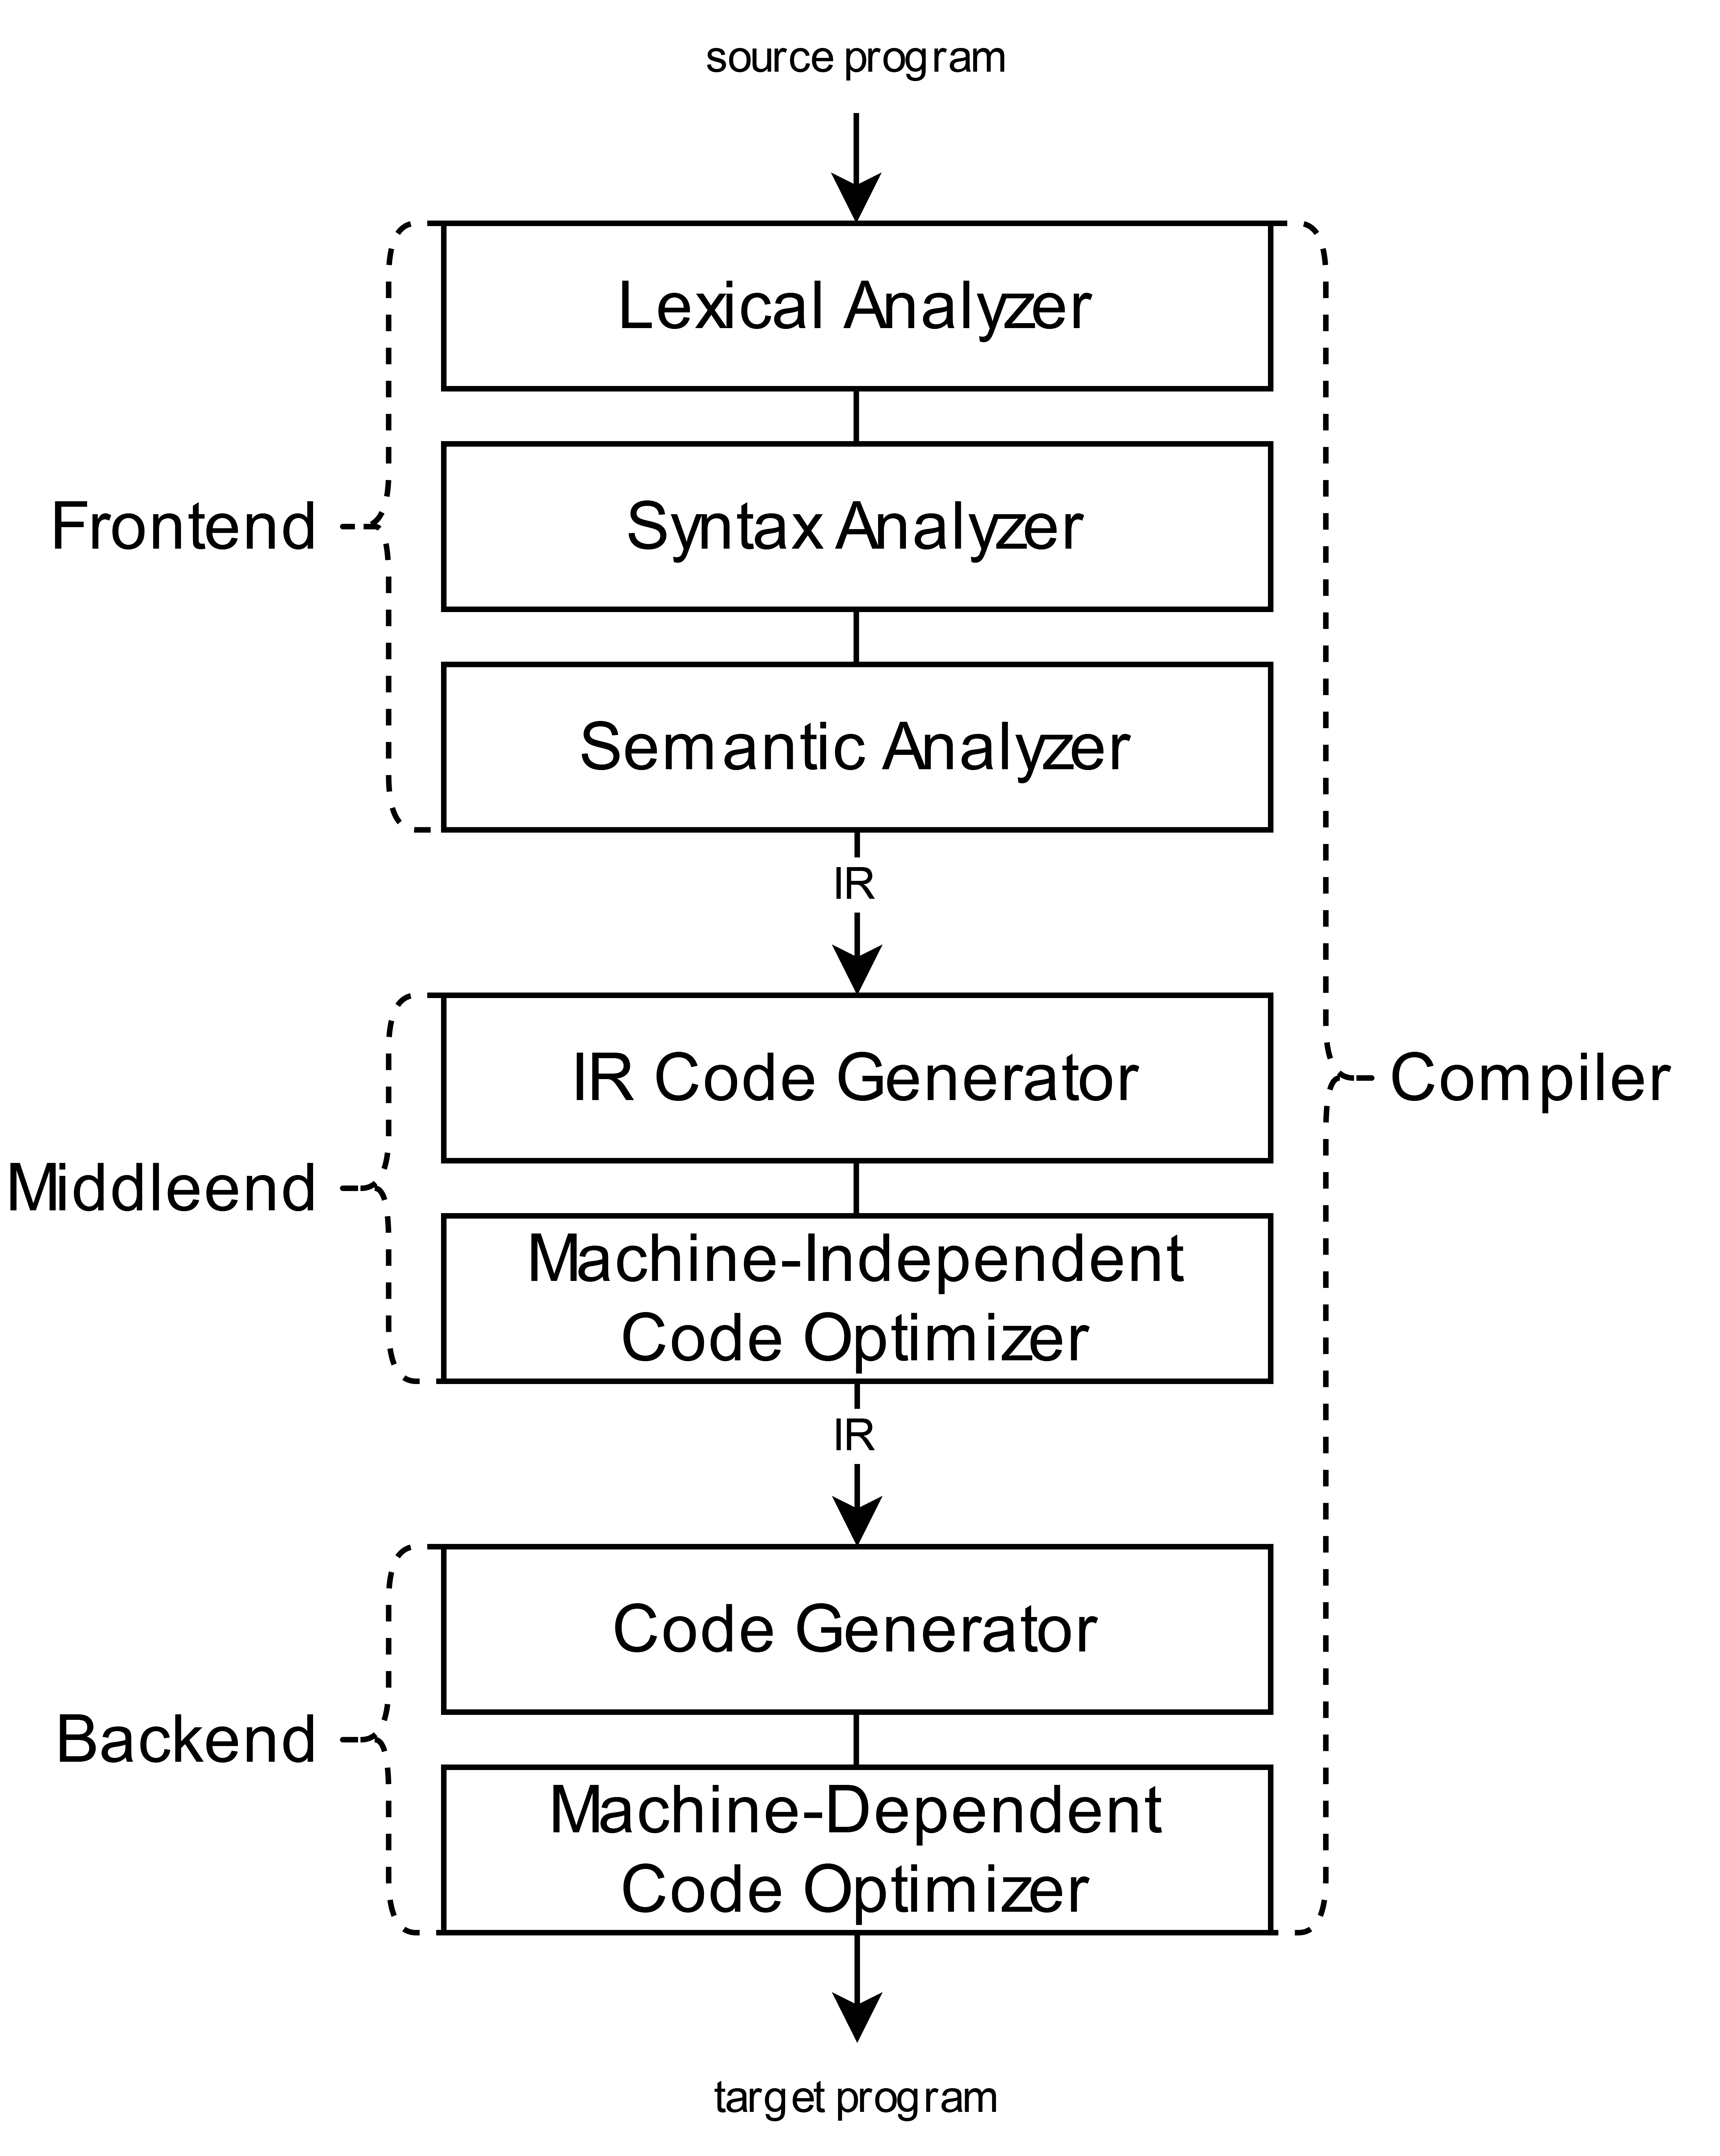
\includegraphics[width=9cm]{img/modern_compiler.png}
    \caption[The three stages of a compilation.]{The three stages of a compilation (inspired by \cite[Fig. 1.6]{dragonbook}).}\label{fig:three_stage_compiler}
\end{figure}

\paragraph*{Frontend} The frontend takes the input source program, parses it and verifies its syntax and semantics. Any syntactic or semantic error gets reported, typically with a source location of the error. The frontend then encodes the input program in some structure for later use by the middleend. This \emph{intermediate representation} (IR) becomes the compiler's definitive representation for the code it is translating \cite[Chap. 1.2]{eng_comp}. The IR is usually a lower-level representation of the program compared to the original source.

\paragraph*{Middleend} The middleend performs various analyses (we will discuss some of them at the end of this chapter) on the IR\footnote{The IR that middleend uses can either be the one provided by the frontend or it can be a different one, generated from the IR provided by the frontend.} and based on the results of these analyses it performs optimizations that are independent on the target architecture. The middleend can perform multiple of these passes, since some optimizations can enable new optimization possibilities that were not available before. Optimized IR is then passed to the backend.

\paragraph*{Backend} The backend is responsible for mapping the IR passed by the middleend into the target program language (this process is called a \emph{code generation}). Backend usually also performs optimizations that are dependent on the target machine. The output of the backend is a target program.

\paragraph*{} This three-stage modularization makes it possible to combine different frontends and backends while sharing the same middleend optimizations. Some examples of this modularization are the \emph{GNU Compiler Collection}\footnote{\url{https://gcc.gnu.org/}} (GCC) or \emph{LLVM}\footnote{\url{https://www.llvm.org/}}, which both have multiple frontends and backends.

\section{MicroC}
The \emph{microC} (stylized as \emph{$\mu$C}) language is a tiny programming language used in the NI-APR course to implement various program analyses. It is based on the TIP (tiny imperative programming language) introduced in \emph{Static Program Analysis} \cite{spa}, which is used as the main course book in the NI-APR course. For example of an iterative and recursive factorial program written in microC see \autoref{lst:microc_example}.

In the next few subsections, we take a look at the structure of the microC language. The description of each language feature is taken from NI-APR \cite{microc}. Abstract syntax of the microC language is defined in \autoref{chap:microC}. In this thesis, we extend the language with support for arrays, which is not yet (as of 4. 4. 2022) officially part of the course, but planned to be added.

\begin{listing}
\centering
\begin{minipage}{.4\linewidth}
	\inputminted[tabsize=2,breaklines,bgcolor=codebg,escapeinside=||]{python}{snippets/microc_fac_iter.m}
\end{minipage}%
\hskip0.2cm
\begin{minipage}{.5\linewidth}
	\inputminted[tabsize=2,breaklines,bgcolor=codebg,escapeinside=||]{python}{snippets/microc_fac_rec.m}
\end{minipage}%
	\caption{Example of iterative and recursive factorial written in microC.}
	\label{lst:microc_example}
\end{listing}

\subsection{Expression}
\paragraph*{Identifier}
The identifier is any name that starts with an underscore or a letter and contains letters, numbers, and underscores only. The only exception are the following reserved keywords: \texttt{alloc}, \texttt{else}, \texttt{if}, \texttt{input}, \texttt{null}, \texttt{output}, \texttt{return}, \texttt{var}, and \texttt{while}.

\paragraph*{Number} A regular 32-bit signed integer.

\paragraph*{Algebraic operators} There are four basic operators for addition, subtraction, multiplication, and division. Their semantic is defined only for numbers, and their precedence is the same as in maths.
\begin{minted}[tabsize=2,breaklines]{python}
x = 2 * 20 + 2;
y = (50 - 8) / 1;
\end{minted}

\paragraph*{Comparison operators} There are two operators for comparison. The \emph{equality}, which allows comparing numbers and pointers, and the \emph{greater than} operator, which allows comparing numbers only. Both yield 1 if the comparison is true, 0 otherwise.
\begin{minted}[tabsize=2,breaklines]{python}
x = 20 == 10;
y = 20 > 10;
\end{minted}

\paragraph*{Input} Reads an integer from standard input. It converts the input into a number or $-1$ in the case end-of-file (EOF) is reached.
\begin{minted}[tabsize=2,breaklines,escapeinside=||]{python}
x = input;
\end{minted}

\paragraph*{Function call} A function call consists of one expression, which evaluates to a function value and zero or more expressions, which are the arguments of the function call. Calls use call-by-value semantics and support recursion.
\begin{minted}[tabsize=2,breaklines]{python}
x = foo(42);
\end{minted}

\paragraph*{Pointer} The microC pointers can be recursive (i.e., pointer to a pointer), but no pointer arithmetic is supported. The \texttt{alloc} expression allocates an expression on the heap and returns a pointer to it. The \texttt{null} expression represents an empty pointer. The dereference operator returns a value that the pointer points to. The reference operator returns a pointer to a variable.
\begin{minted}[tabsize=2,breaklines,escapeinside=||]{python}
x = |\microcalloc| 42;
y = *x;
z = &x;
x = |\microcnull|;
\end{minted}

\paragraph*{Record} A record is a value that is composed of one or more fields. Once a record type is assigned to a variable, its fields are fixed and it is not possible to add more fields later. A field can contain any value, except for records, but it can contain a pointer to a record. Records are stack allocated.
\begin{minted}[tabsize=2,breaklines]{python}
x = { a: 0, b: 1, c: 2 };
\end{minted}

\paragraph*{Array} An array is a sequence of fixed length that contains values of the same type. It can contain any value, except for arrays. Arrays are stack allocated.
\begin{minted}[tabsize=2,breaklines]{python}
x = [ 0, 1, 2 ];
\end{minted}

\paragraph*{Comment} The language supports C-style single line and block comments.
\begin{minted}[tabsize=2,breaklines]{cpp}
//single line
/*
    multi
    line
*/
\end{minted}

\subsection{Statement}
\paragraph*{Assignment} There are five kinds of assignments in microC:
\begin{itemize}
    \item Direct write---a write to a variable.
\begin{minted}[tabsize=2,breaklines]{python}
x = y;
\end{minted}
    \item Indirect write---a write to a memory location referenced by a pointer.
\begin{minted}[tabsize=2,breaklines]{python}
*x = y;
\end{minted}
    \item Direct field write---a write to a record field.
\begin{minted}[tabsize=2,breaklines]{python}
x.a = y;
\end{minted}
    \item Indirect field write---a write into a field of a record that is referenced by a pointer.
\begin{minted}[tabsize=2,breaklines]{python}
(*x).a = y;
\end{minted}
    \item Array write---a write to an array element.
\begin{minted}[tabsize=2,breaklines]{python}
x[0] = y;
\end{minted}
\end{itemize}

\paragraph*{If conditional} In the conditional, only 0 is interpreted as \emph{false}, everything else is interpreted as \emph{true}. The \emph{else} branch of the conditional is optional.
\begin{minted}[tabsize=2,breaklines]{python}
if (x) {
    y = 42;
} else {
    y = -42;
}
\end{minted}

\paragraph*{While loop} Repeatedly executes its body as long as its guarding condition evaluates to \emph{true} (any non-0 value).
\begin{minted}[tabsize=2,breaklines]{python}
while (x) {
  x = x - 1;
}
\end{minted}

\paragraph*{Output} Writes a single integer (i.e., an expression that evaluates to an integer) into the standard output.
\begin{minted}[tabsize=2,breaklines,escapeinside=||]{python}
|\microcoutput| 42;
\end{minted}

\paragraph*{Block} A sequence of other statements (including other blocks) surrounded by curly brackets.

\subsection{Function} Each function has a unique name, takes zero or more arguments, and defines zero or more local variables. All variables are defined at the top of the function. The function has a single return defined at the end of the function body. The function body is a sequence of statements. Functions are also treated as first-class citizens\footnote{Values or objects, that can be passed as an argument, returned from a function, and assigned to a variable.}, but the language does not support pointers to functions.
\begin{minted}[tabsize=2,breaklines,escapeinside=||]{python}
main() {
    |\microcvar| f;
    f = foo;
    return f(42);
}
\end{minted}

\subsection{Program} A microC program is a simple collection of functions. The entry and exit point of the program is conventionally a function named \emph{main}, which is restricted to take no arguments and return an integer.


\section{x86-64}\label{sec:x86-64}
Intel's \emph{x86-64 ISA}\footnote{Instruction Set Architecture} (also known as \emph{Intel 64}) is a 64-bit extension of the original x86 ISA. The x86-64 is a \emph{Complex Instruction Set Computing} (CISC) CPU design, which typically include a wide variety of instructions with varying sizes and wide range of addressing modes \cite[Chap. 1.0]{x86_assembly}. Complete instruction set of x86-64 is available from \cite{intel_x86}.

As mentioned in the introduction of this thesis, x86-64 will be the target language of our compiler. More specifically, the output of the compiler will be x86-64 assembly code (see \autoref{lst:x86_example} for an example) executable under any Linux-based 64-bit OS.

\begin{listing}
	\inputminted[tabsize=2,breaklines,bgcolor=codebg]{asm}{snippets/x86_example.m}
	\caption{Example of an x86-64 assembly code.}
	\label{lst:x86_example}
\end{listing}

\subsection{Storage organization}\label{ssec:storage_org}
From our perspective, the executing target program runs in its own address space, in which each program value has a location. The management and organization of this address space is shared between the compiler, operating system, and the target machine \cite[Chap. 7.1]{dragonbook}.

That's why it's important to get more familiar with the storage organization of a program running on the x86 target machine. That way we can get better understanding of, for example, where local variables are stored or how are arguments passed to a function.

Memory layout of a running x86 program generally consists of a lot of segments, however we will be focusing only on a few of them. Their arrangement is shown in \autoref{fig:x86_memory}, which is a simplified version of \cite[Fig. 6-1]{linux_interface}.

\paragraph*{Stack} When a function is called, the machine allocates a chunk of stack memory for it---this chunk is often referred to as a \emph{stack frame} and it contains all the local variables of the function, arguments of the function, and temporary values. These values are accessed using addresses relative to stack pointer\footnote{\emph{Stack pointer} is a pointer that points to the current top of the stack \cite[Chap. 2.3.1.2]{x86_assembly}.} (SP) and base pointer\footnote{\emph{Base pointer} points to the start of a function's stack frame \cite[Chap. 2.3.1.3]{x86_assembly}.} (BP) \cite[Chap. 12.11]{calling_convention}. When the function is returning, the stack frame is deallocated and all of its local variables and arguments become invalid. This allocation and deallocation is a responsibility of the compiler, and it will be discussed in the following chapter.

\paragraph*{Heap} The area for dynamically allocated memory is called the heap. One of the key differences between stack and heap memory is the responsibility for allocation and deallocation. Heap memory is allocated explicitly by a programmer and variables allocated on it never fall out of scope like local variables on the stack. To allocate heap memory in C++ we use keyword \texttt{new}. In microC, the keyword \texttt{alloc} is used.

\paragraph*{Data} This section stores global and static variables. It is further divided into initialized and uninitialized data segments. Since in microC functions are first-class citizens and they are treated like ordinary variables, this is where they will be stored (since they are accessible from any other scope, i.e., they are global).

\paragraph*{Text} Text segment is a memory section that contains the code that is being executed. In order to prevent a program from accidentally modifying its instruction, this section is read-only.
\begin{figure}
    \centering
    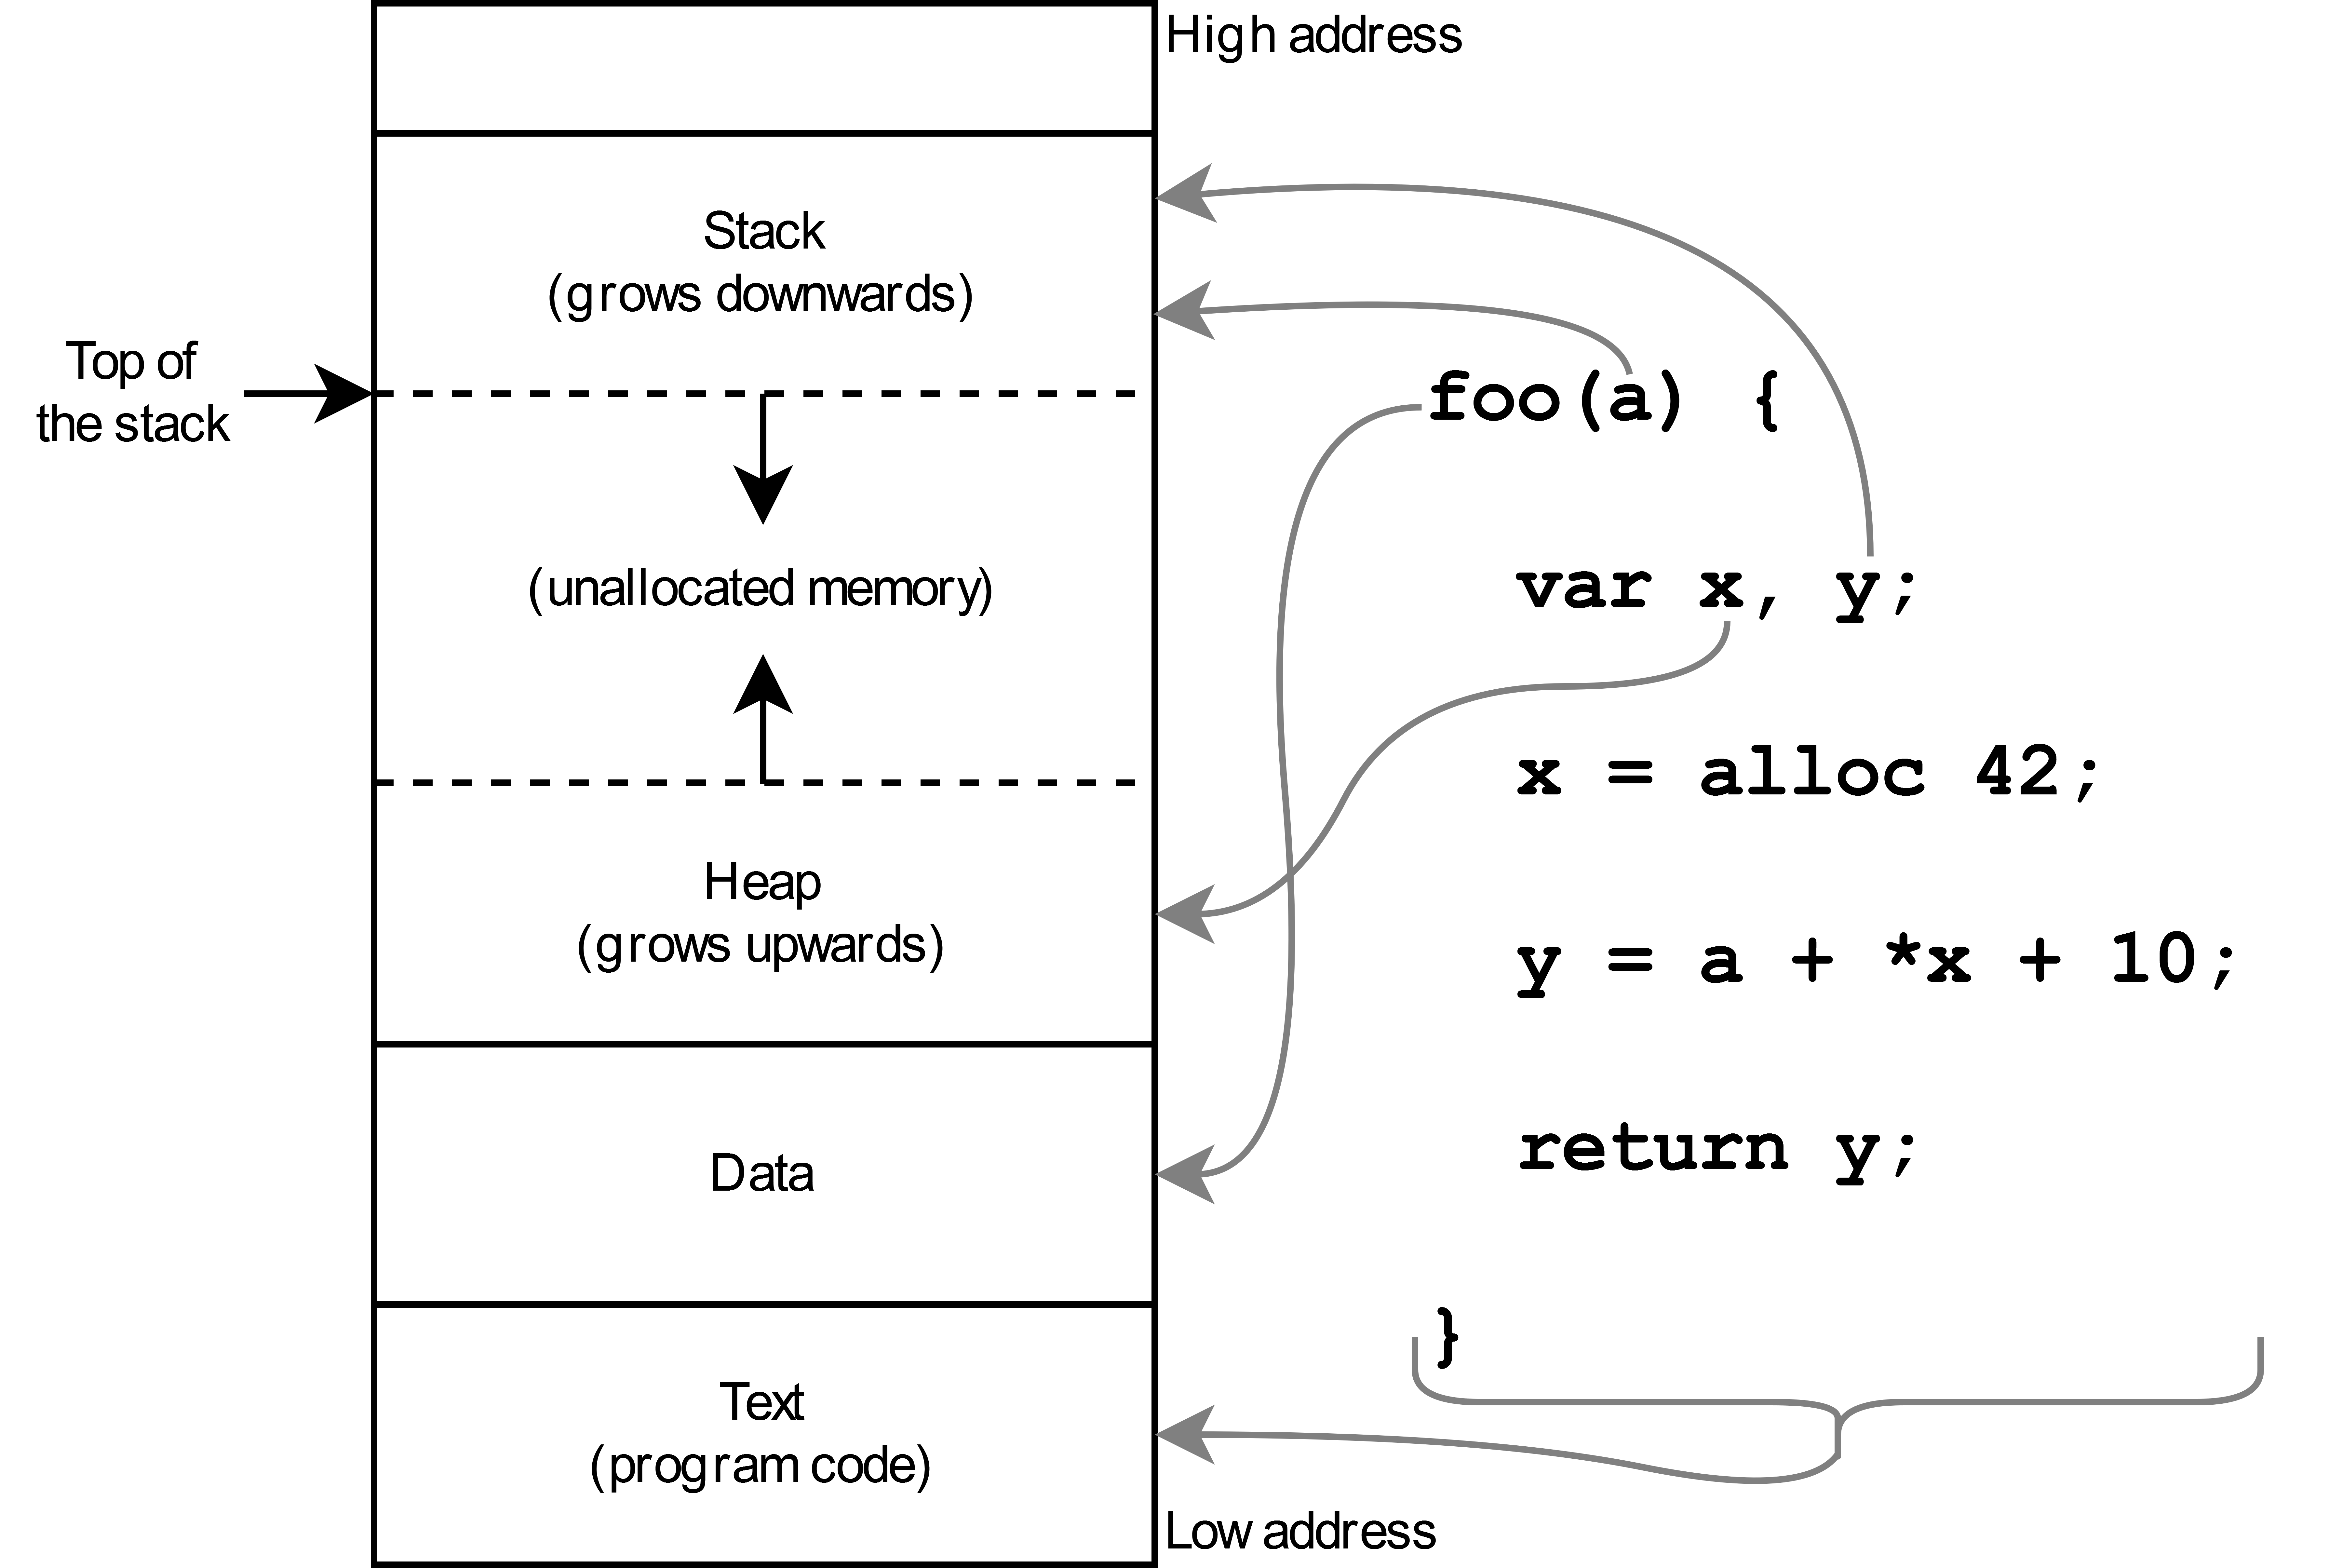
\includegraphics[width=12cm]{img/x86memory}
    \caption{Typical memory layout of a running x86 program.}\label{fig:x86_memory}
\end{figure}


\section{Static program analysis}\label{sec:analyses}
\emph{Static program analyses} are used to reason about the behaviour of computer programs without actually running them \cite[Preface]{spa}. This is useful for many purposes, such as:
\begin{itemize}
    \item Program optimization---e.g., detecting unused and unreachable code which can be deleted by the optimizer, detecting variables whose value can be computed at compile time, deciding if two pointers point to the same data structure, or determining bounds of an integer variable.
    \item Program correctness---e.g., deciding if the program is typeable\footnote{A program is \emph{typeable} if it satisfies a collection of type constraints derived from the program \cite[Chap. 3]{spa}.}, detecting use of an undeclared variable, checking if all variables are initialized before they are read, or determining if the program terminates on every possible input.
    \item Program development---supporting various tools of modern IDEs like debugging, refactoring, code completion, type inference, or detecting where a function can be called from.
\end{itemize}

In this section, we will get more familiar with some of the analyses used for the first two listed purposes, as those will be utilized in our compiler. The following subsections will use \autoref{lst:analysis_example} as an example of an analysed microC program snippet.

\begin{listing}
	\inputminted[tabsize=2,breaklines,bgcolor=codebg,escapeinside=||]{python}{snippets/analysis_example.m}
	\caption{Example of an analysed microC program snippet.}
	\label{lst:analysis_example}
\end{listing}

\subsection{Semantic analysis}
The \emph{semantic analysis} is an example of an analysis for program correctness. The version that we will use in our compiler checks the following:
\begin{itemize}
    \item Use of an undeclared identifier.
    \item Duplicate identifiers.
    \item Duplicate record field names.
    \item Assignment to a function.
    \item Taking an address of a function.
\end{itemize}

The output of semantic analysis is a mapping of identifiers to their declaration in the program.

\subsection{Type analysis}
The \emph{type analysis} is another example of an analysis for program correctness. Its goal is to assign type to each value of a program and decide if the program is typeable. This will prevent the compiler to even process ill-typed programs. The output of type analysis is a mapping of variable declarations to their respective types. Example of a type analysis output for the program from \autoref{lst:analysis_example}:
\begin{align*}
    [\![ x ]\!] &= int \\
    [\![ y ]\!] &= \{ a : int \}
\end{align*}

\subsection{Control flow graph}\label{ssec:cfg}
Each of the so far mentioned analyses works with a representation of a program without the need to know the actual dataflow of the program. However, this is not the case for all the analyses we will be talking about. Some of the analyses (which are referred to as \emph{dataflow analyses}) require the knowledge of program's dataflow. For this purpose it is more convenient to work with a different representation of the program called \emph{control flow graph}.

A control flow graph (CFG) is a directed graph, in which \emph{nodes} correspond to statements and \emph{edges} represent possible flow of control \cite[Chap. 2.5]{spa}. A CFG of a microC program always has a single point of entry (denoted \emph{entry}) and a single point of exit (denoted \emph{exit}). An example of a CFG is shown in \autoref{fig:cfg}.

\begin{figure}
    \centering
    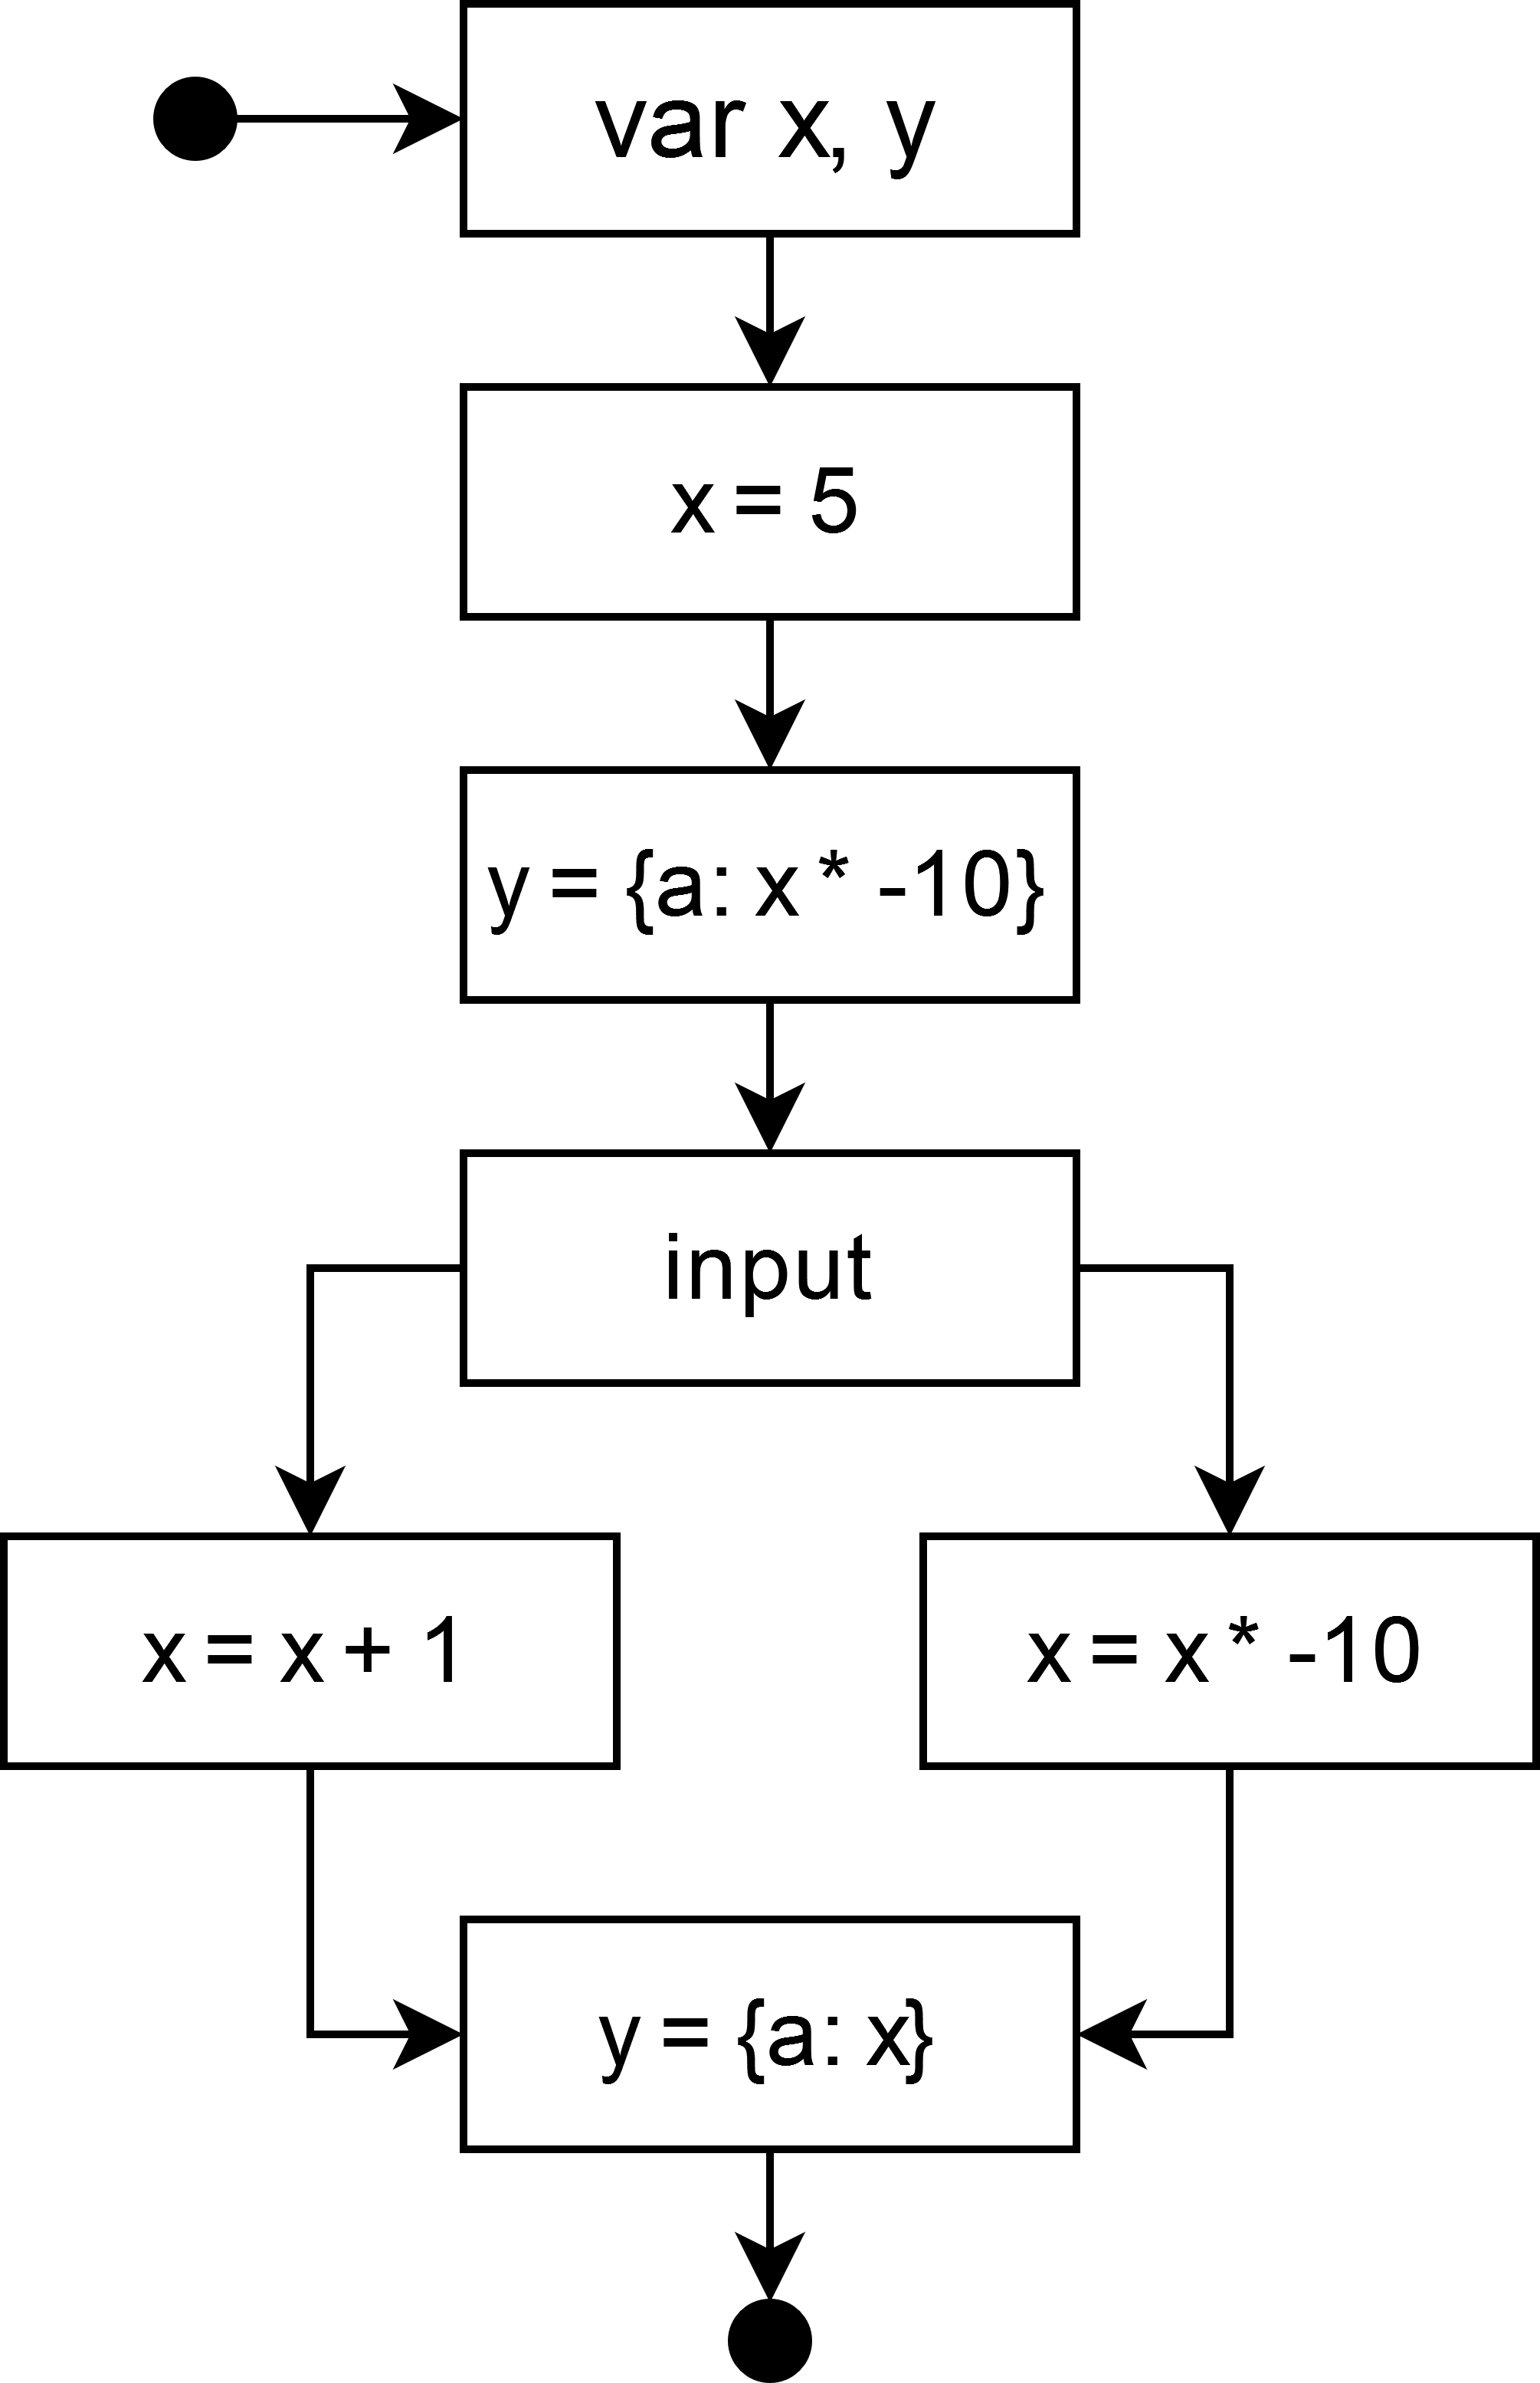
\includegraphics[height=8cm]{img/cfg}
    \caption{CFG of the program snippet from \autoref{lst:analysis_example}.}\label{fig:cfg}
\end{figure}

\subsection{Sign analysis}
The \emph{sign analysis} is an example of a dataflow analysis for program optimization. Its goal is to determine what sign (+, -, or 0) each expression has, which the compiler can then use to simplify certain binary operations\footnote{E.g., a binary operation \emph{equals to} between positive and negative integer will always evaluate to \texttt{false}.}. The output of sign analysis is a mapping of CFG nodes to maps from declaration to sign or abstract values $\top$ (representing “don't know”, i.e., the sign of the declaration is uncertain) and $\bot$ (representing uninitialized values)\footnote{More details about these abstract values can be found in \cite[Chap. 4]{spa}, which covers the \emph{Lattice Theory}.}. This output tells us what are the signs of variables \emph{after} the given CFG node. Example output for the program from \autoref{lst:analysis_example} (the “$[\![ \emph{entry} ]\!]$” notion denotes a CFG node):

\begin{align*}
    [\![ \emph{entry} ]\!] &= \{ x \rightarrow \bot, y \rightarrow \bot \}\\
    [\![ \texttt{var x,y} ]\!] &= \{ x \rightarrow \bot, y \rightarrow \bot \}\\
    [\![ \texttt{x=5} ]\!] &= \{ x \rightarrow +, y \rightarrow \bot \}\\
    [\![ \texttt{y=\{a:x*-10\}} ]\!] &= \{ x \rightarrow +, y \rightarrow \top \}\\
    [\![ \texttt{input} ]\!] &= \{ x \rightarrow +, y \rightarrow \top \}\\
    [\![ \texttt{x=x+1} ]\!] &= \{ x \rightarrow +, y \rightarrow \top \}\\
    [\![ \texttt{x=x*-10} ]\!] &= \{ x \rightarrow -, y \rightarrow \top \}\\
    [\![ \texttt{y=\{a:x\}} ]\!] &= \{ x \rightarrow \top, y \rightarrow \top \}\\
    [\![ \emph{exit} ]\!] &= \{ x \rightarrow \top, y \rightarrow \top \}
\end{align*}

We can see from the output that after the CFG node $[\![ \texttt{y=\{a:x\}} ]\!]$ the sign of the variable \texttt{x} is uncertain, because it could be either $+$ or $-$, based on which integer the expression \texttt{input} evaluates to.

\subsection{Constant propagation analysis}\label{ssec:constant_prop_analysis}
The \emph{constant propagation} analysis is very similar to the sign analysis. The only difference is that the goal is to determine which variables have a constant value (0, 1, etc.). This knowledge can then be used to simplify certain expressions that can be evaluated during compile time. Output of the analysis is a mapping of CFG nodes to maps from declaration to constant value, $\top$, or $\bot$. This output tells us what are the constant values of variables \emph{after} the given CFG node. Example output for the program from \autoref{lst:analysis_example}:

\begin{align*}
    [\![ \emph{entry} ]\!] &= \{ x \rightarrow \bot, y \rightarrow \bot \}\\
    [\![ \texttt{var x,y} ]\!] &= \{ x \rightarrow \bot, y \rightarrow \bot \}\\
    [\![ \texttt{x=5} ]\!] &= \{ x \rightarrow 5, y \rightarrow \bot \}\\
    [\![ \texttt{y=\{a:x*-10\}} ]\!] &= \{ x \rightarrow 5, y \rightarrow \top \}\\
    [\![ \texttt{input} ]\!] &= \{ x \rightarrow 5, y \rightarrow \top \}\\
    [\![ \texttt{x=x+1} ]\!] &= \{ x \rightarrow 6, y \rightarrow \top \}\\
    [\![ \texttt{x=x*-10} ]\!] &= \{ x \rightarrow -50, y \rightarrow \top \}\\
    [\![ \texttt{y=\{a:x\}} ]\!] &= \{ x \rightarrow \top, y \rightarrow \top \}\\
    [\![ \emph{exit} ]\!] &= \{ x \rightarrow \top, y \rightarrow \top \}
\end{align*}

An optimizing compiler will use this output to, for example, propagate the value of the variable \texttt{x} into the CFG node $[\![ \texttt{y=\{a:x*-10\}} ]\!]$. The statement of the CFG node will be optimized to \texttt{y=\{a:5*-10\}}, which can then be further optimized to \texttt{y=\{a:-50\}}.

\subsection{Live variable analysis}\label{ssec:live_var_analysis}
The \emph{live variable analysis} is a dataflow analysis used for program optimization. It calculates which variables are \emph{live} at each point in the program. The compiler can then use this knowledge to optimize variables that are \emph{dead} (i.e., they hold a value that won't be read before the next time they are written to), since they don't need to be stored. The output of the analysis is a mapping of CFG nodes to a set of live variables. This output tells us which variables are live \emph{before} the given CFG node. Example output for the program from \autoref{lst:analysis_example}:

\begin{align*}
    [\![ \emph{entry} ]\!] &= \emptyset\\
    [\![ \texttt{var x,y} ]\!] &= \emptyset\\
    [\![ \texttt{x=5} ]\!] &= \emptyset\\
    [\![ \texttt{y=\{a:x*-10\}} ]\!] &= \{ x \}\\
    [\![ \texttt{input} ]\!] &= \{ x \}\\
    [\![ \texttt{x=x+1} ]\!] &= \{ x \}\\
    [\![ \texttt{x=x*-10} ]\!] &= \{ x \}\\
    [\![ \texttt{y=\{a:x\}} ]\!] &= \{ x \}\\
    [\![ \emph{exit} ]\!] &= \emptyset
\end{align*}

We can see that at no point in the program is the variable \texttt{y} live. An optimizing compiler will use this information to eliminate both assignments to \texttt{y}, since there is no point in storing dead variables.

\subsection{Available expression analysis}
A non-trivial expression\footnote{In microC it's the binary operation.} is \emph{available} at a program point if its current value has been computed earlier in the execution \cite[Chap. 5.5]{spa}. The goal of the \emph{available expression analysis} is to determine which expressions are available at the given program point. Output of the analysis is a mapping of CFG nodes to sets of available expressions. This output tells us which expressions are available \emph{after} the given CFG node. Example output for the program from \autoref{lst:analysis_example}:

\begin{align*}
    [\![ \emph{entry} ]\!] &= \emptyset\\
    [\![ \texttt{var x,y} ]\!] &= \emptyset\\
    [\![ \texttt{x=5} ]\!] &= \emptyset\\
    [\![ \texttt{y=\{a:x*-10\}} ]\!] &= \{ \texttt{(x*-10)} \}\\
    [\![ \texttt{input} ]\!] &= \{ \texttt{(x*-10)} \}\\
    [\![ \texttt{x=x+1} ]\!] &= \emptyset\\
    [\![ \texttt{x=x*-10} ]\!] &= \emptyset\\
    [\![ \texttt{y=\{a:x\}} ]\!] &= \emptyset\\
    [\![ \emph{exit} ]\!] &= \emptyset\\
\end{align*}

Since the value of the variable \texttt{x} changes in both of the branching CFG nodes $[\![ \texttt{x=x+1} ]\!]$ and $[\![ \texttt{x=x*-10} ]\!]$, the expression \texttt{(x*-10)} is no longer available after them and cannot be reused.

\chapter{Design}
Armed with knowledge from the previous chapter, we are ready to discuss the design of the microC compiler. Our main goal is to create a compiler, that can be easily plugged with the results of the various static analyses covered in the NI-APR course. These results will be utilized in various optimizations performed by the compiler. In this chapter, we discuss the design of each part of the compiler, mainly middleend and backend.

\section{The frontend}\label{sec:frontend}
As described in \autoref{ssec:modularization}, the responsibility of a compiler's frontend is to parse the input source program and produce an IR that will be used in the compiler's middleend. For this purpose, we can use the parser provided to students in the NI-APR course, which parses the input microC program and produces an \emph{abstract syntax tree}\footnote{\emph{Abstract syntax tree} represents the hierarchical syntactic structure of the source program~\cite[Chap. 2.1]{dragonbook}.} (AST) representation of the program.

The advantage of this choice is that students of the NI-APR course will already be familiar with the output of the parser. Since there is no need to further modify it, we will use the AST as an output IR of the compiler's frontend (for illustration, see \autoref{fig:microc_frontend}).

\begin{figure}
    \centering
    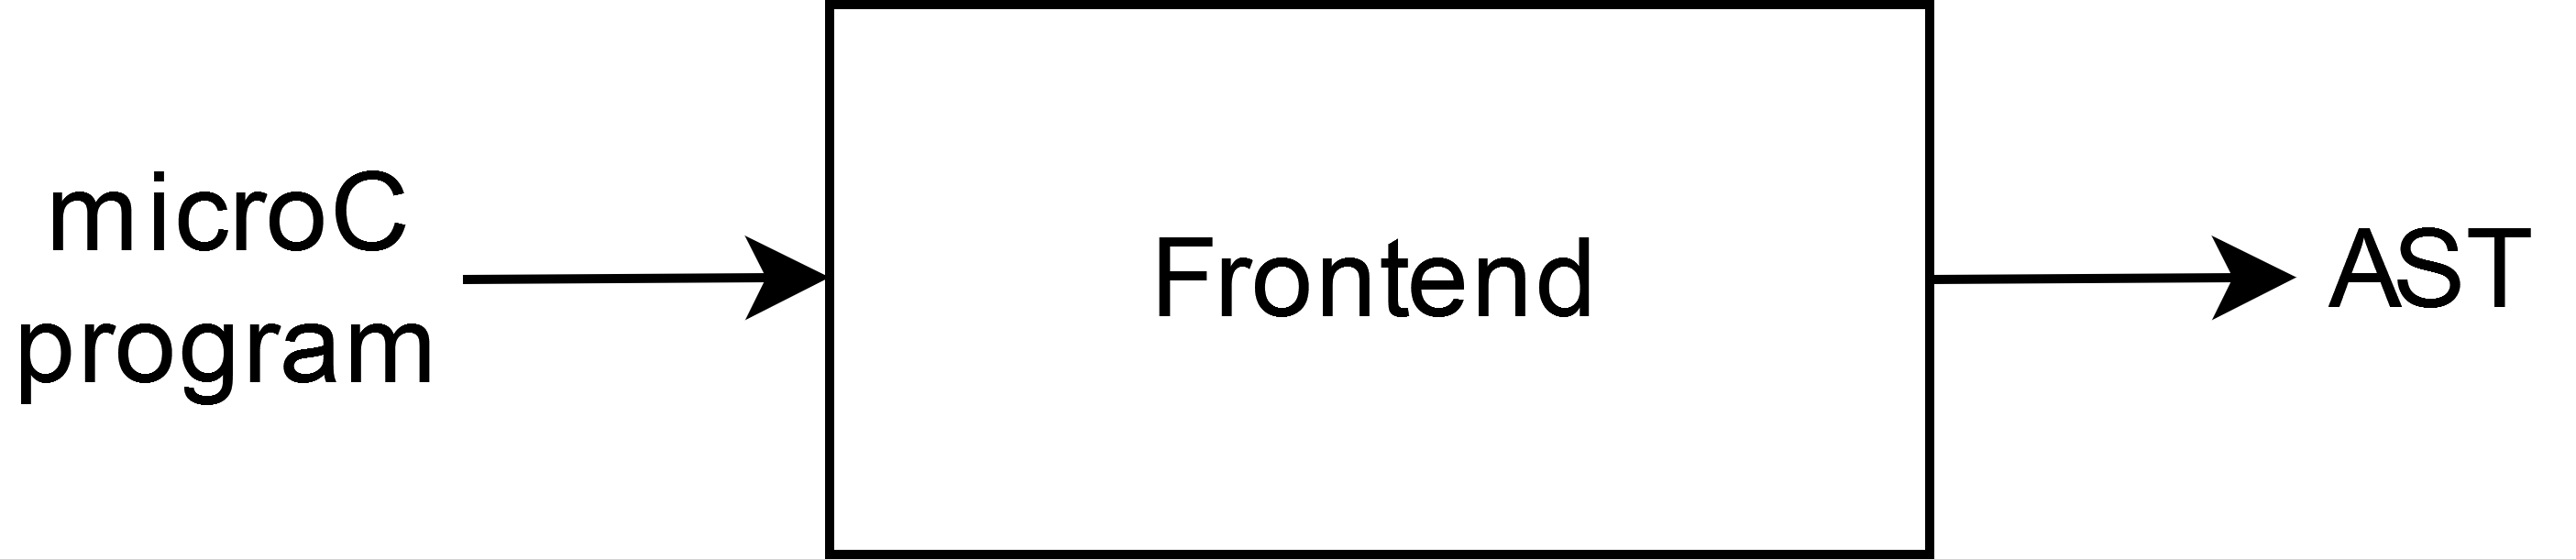
\includegraphics[width=8cm]{img/microc_frontend.png}
    \caption{The frontend of the microC compiler.}\label{fig:microc_frontend}
\end{figure}


\section{The middleend}\label{sec:middleend}
The responsibility of our compiler's middleend will be to utilize provided analyses, use them to perform various kinds of optimizations, and then produce IR from which will the backend generate a target program (x86 assembly). However, this is where we run into our first dilemma---what kind of IR should we use to perform optimizations on?

The idea of \emph{optimizing a program} boils down to rewriting a program so that it computes the same answer in a more efficient way \cite[Chap. 1.3.2]{eng_comp}. This means that the IR representing a program should be easily modifiable. One option would be to use the IR provided by the frontend---the AST. However, this representation is not well-suited for modifications (since it was not designed for this purpose in the first place). That is why we will go with the second logical option---defining a new IR, that will be well-suited for modifications performed by the optimizer. We will discuss the design of such IR in the following subsection.

\subsection{CFG as an IR}\label{ssec:cfg_as_ir}
In the \autoref{ssec:cfg} we introduced a notion of a CFG. This representation of a program will be used in most of the analyses that will be provided to our compiler. Coincidentally, it is also quite suitable for performing modifications on it. For example, removal of a program statement can be done by removing the corresponding CFG node and reconnecting its edges. Similarly, adding a program statement is done by simply adding a new CFG node. This makes CFG a suitable candidate for our middleend IR.

The advantage of choosing CFG as our middleend IR is that the optimizer will perform optimizations directly on the CFG. The modified CFG can then be immediately used to run another round of analyses and optimizations\footnote{This “round” of analyses and optimizations is often referred to as an \emph{optimization pass}.}, which makes the whole process much simpler. Another advantage is that the NI-APR course already provides a class for constructing CFG from AST called \texttt{IntraproceduralCfgFactory}. This class will be used as a first component of the middleend and its output (the CFG of a program) will be used in another important component of the middleend---the optimizer, which we will discuss in the following subsection.

However, to be able to use CFG in the optimizer and also as an output of the middleend (which will backend use to generate x86 assembly), we will have to tackle one issue that CFG has---the loss of information when it comes to branching. Recall the example CFG from \autoref{fig:cfg}---the if-statement is represented by a branching that starts from the node \texttt{input}. However, the context of this branching (which branch is \emph{then} branch and which is \emph{else}) is lost. The same loss of a context applies to while-statements. To make up for this loss, we will have to extend the CFG with a \emph{context} for each of the nodes of the CFG. The goal of a \emph{CFG node context} will be to provide additional information about the given CFG node and its branching. There will be four types of contexts in total:
\begin{itemize}
    \item \emph{Basic Context}---context of a CFG node that is not introducing any form of a branching.
    \item \emph{If Context}---context of a CFG node that is introducing branching via if-statement (e.g., the \texttt{input} node from the example). It will contain information about which branch is \emph{then} and which is \emph{else}.
    \item \emph{While Context}---context of a CFG node that is introducing branching via while-statement. It will contain information about which branch is the body of the while-statement and which is the branch that comes after the while-statement.
    \item \emph{Do-While Context}\footnote{Even though microC does not define do-while-statements, some optimizations will transform while-statements to do-while-statements. Therefore, it is necessary to define a context for do-while-statement.}---context of a CFG node that is the first node of a do-while-statement body. It will contain information about which branch is the body and which is the guard of the do-while-statement.
\end{itemize}

We will discuss implementation of CFG node contexts in detail in the following chapter.

\subsection{Optimizer}\label{ssec:optimizer}
The optimizer is a pivotal component of the compiler's middleend. Its purpose is to take an IR (in our case CFG), perform various kind of optimizations and produce optimized IR. When designing such optimizer, we have to consider following properties that the optimizer should have:
\begin{itemize}
    \item interoperability with the provided analyses, and
    \item extensibility of the optimizer with new optimizations.
\end{itemize}

The idea is to have an optimizer that can be easily provided with analyses and “plugged with” different kinds of optimizations. The more analyses and optimizations will be provided, the more the optimizer will be effective in optimization of a CFG. This idea is illustrated in \autoref{fig:optimizer}.

\begin{figure}
    \centering
    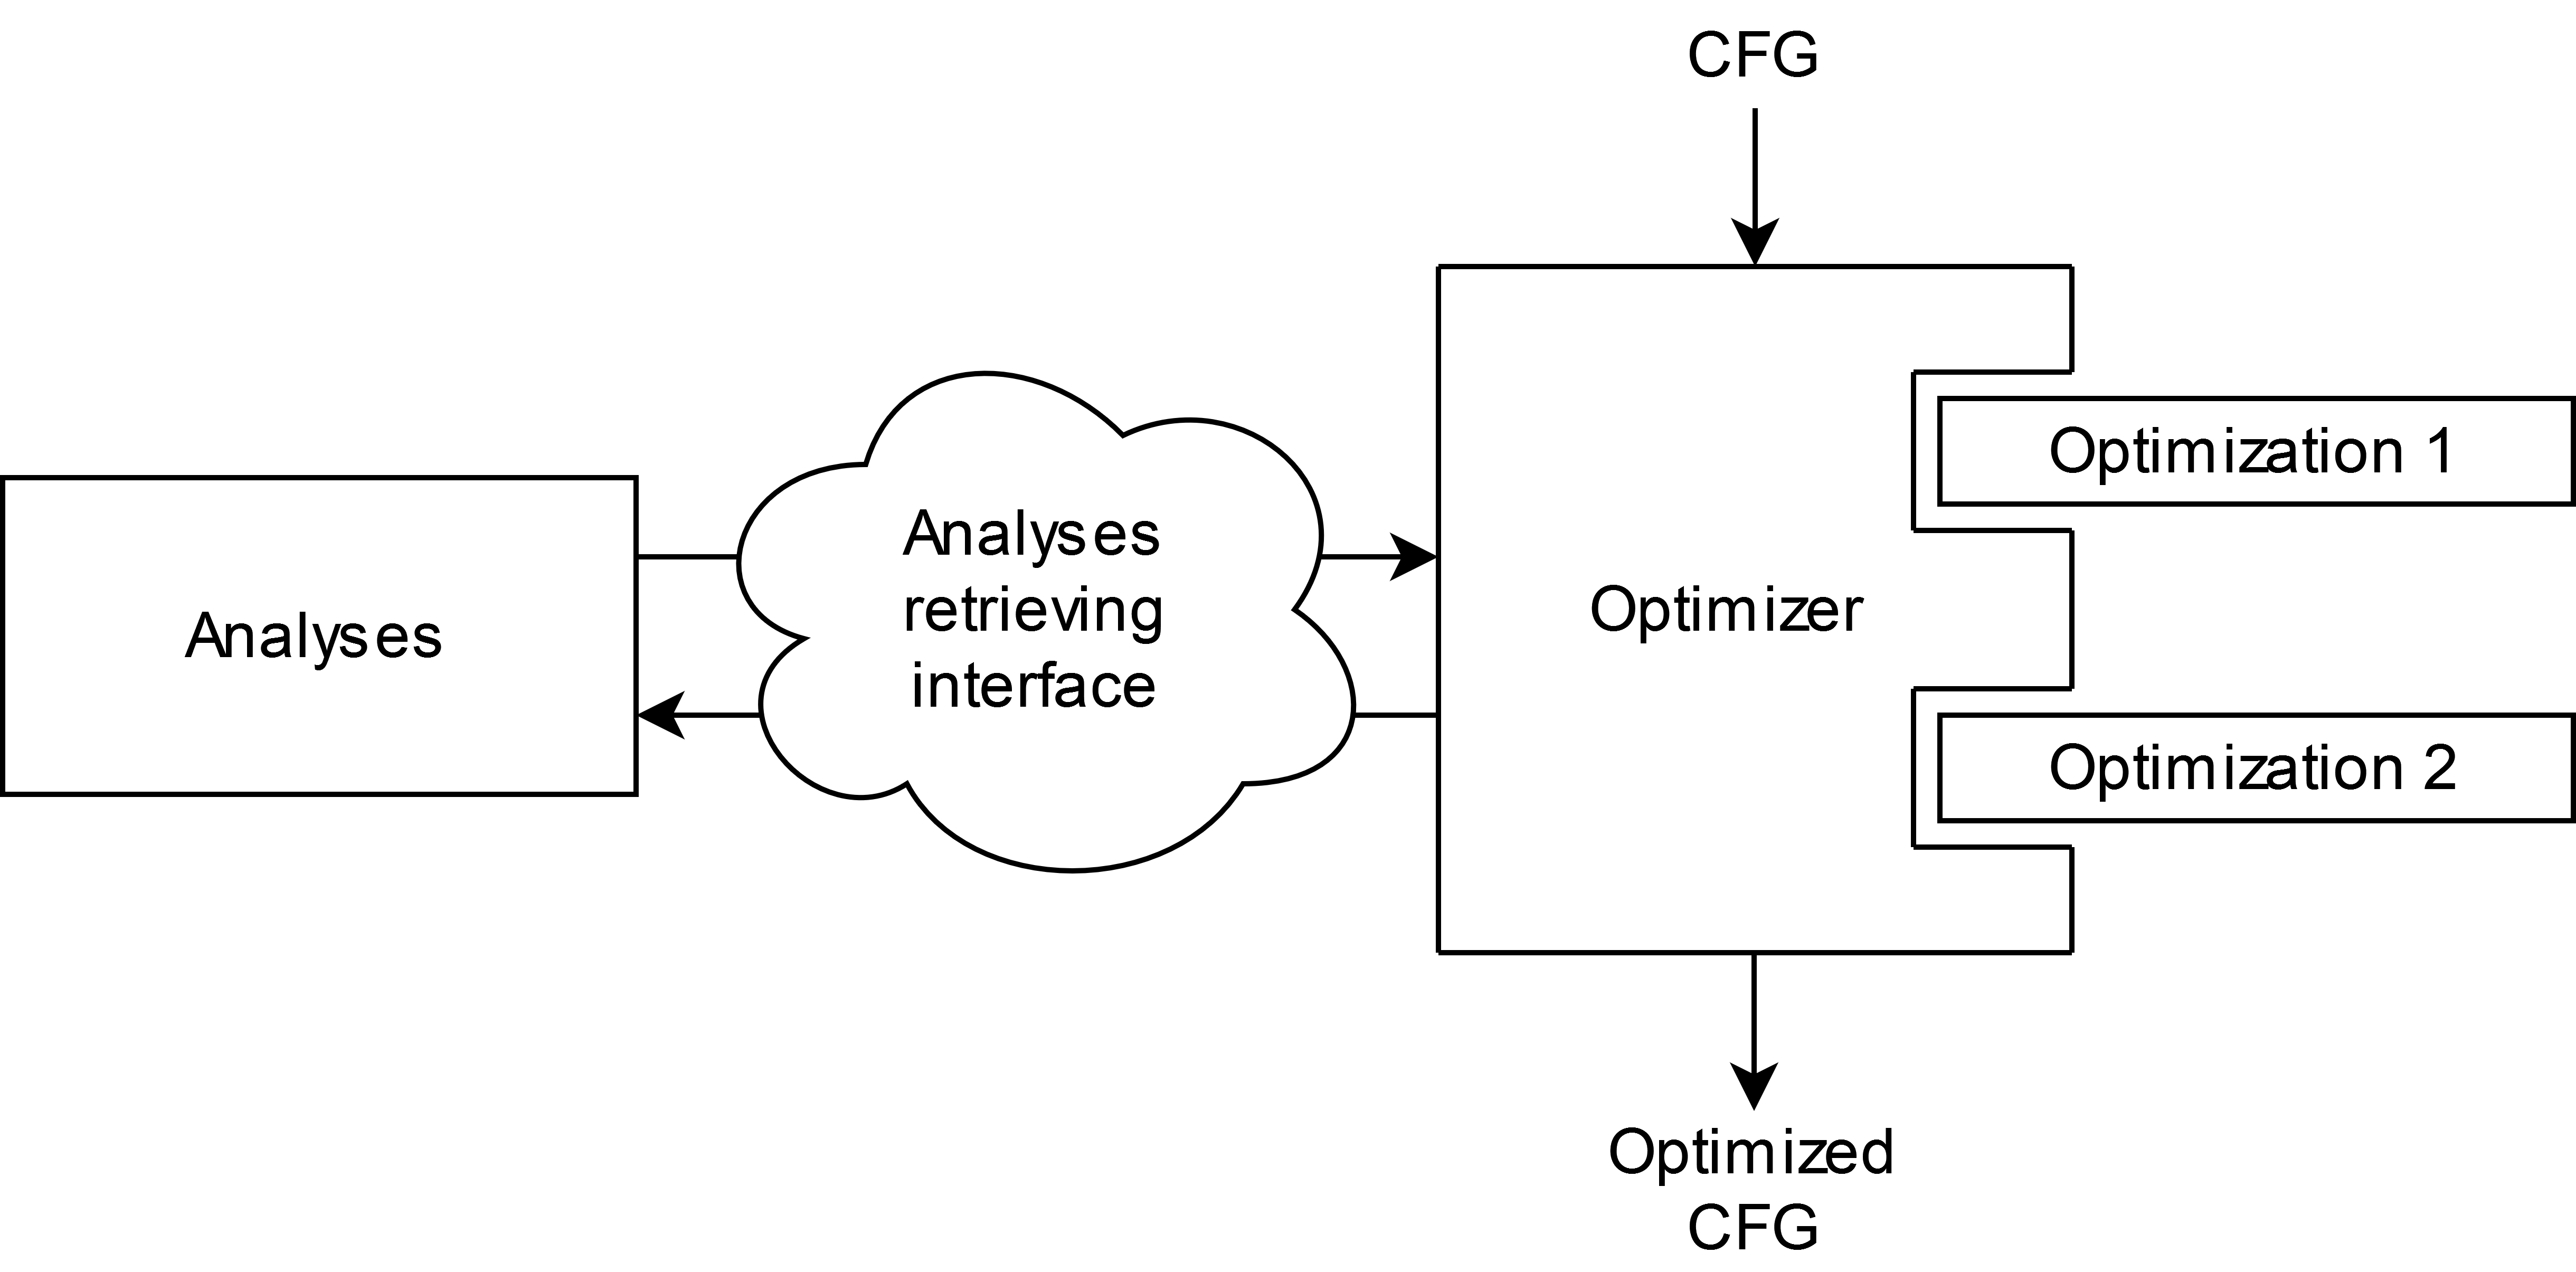
\includegraphics[height=5.5cm]{img/optimizer}
    \caption{An optimizer.}\label{fig:optimizer}
\end{figure}

The interoperability with the provided analyses can be ensured by defining an interface, that will be used to provide analysis with a CFG and retrieve the result of the analysis. Since this is an implementation detail, we will discuss this interface in the following chapter.

To ensure extensibility of the optimizer with new optimizations, we will have to define a unified approach to performing optimizations. Each of the optimizations we will be discussing in the following subsections can be boiled down to a process of observing input CFG, deriving some optimization actions\footnote{E.g., deleting a CFG node, replacing a CFG node with another, introducing a new variable declaration, etc.}, and performing the optimization actions which will modify the input CFG into an optimized one. The last part of this process (performing optimization actions) is identical for all optimizations, therefore an optimization can be “stripped down” to a process that takes CFG together with results of analyses of the CFG and produces a sequence of optimization actions. This approach simplifies addition of new optimizations, since the one who will be designing a new optimization will not have to be concerned with how the optimization actions will be performed (this will be the concern of the optimizer, which will perform said actions). The only concern will be \emph{how to derive those optimization actions}. For better understanding of the whole process of optimization, refer to \autoref{fig:optimizing}.

\begin{figure}
    \centering
    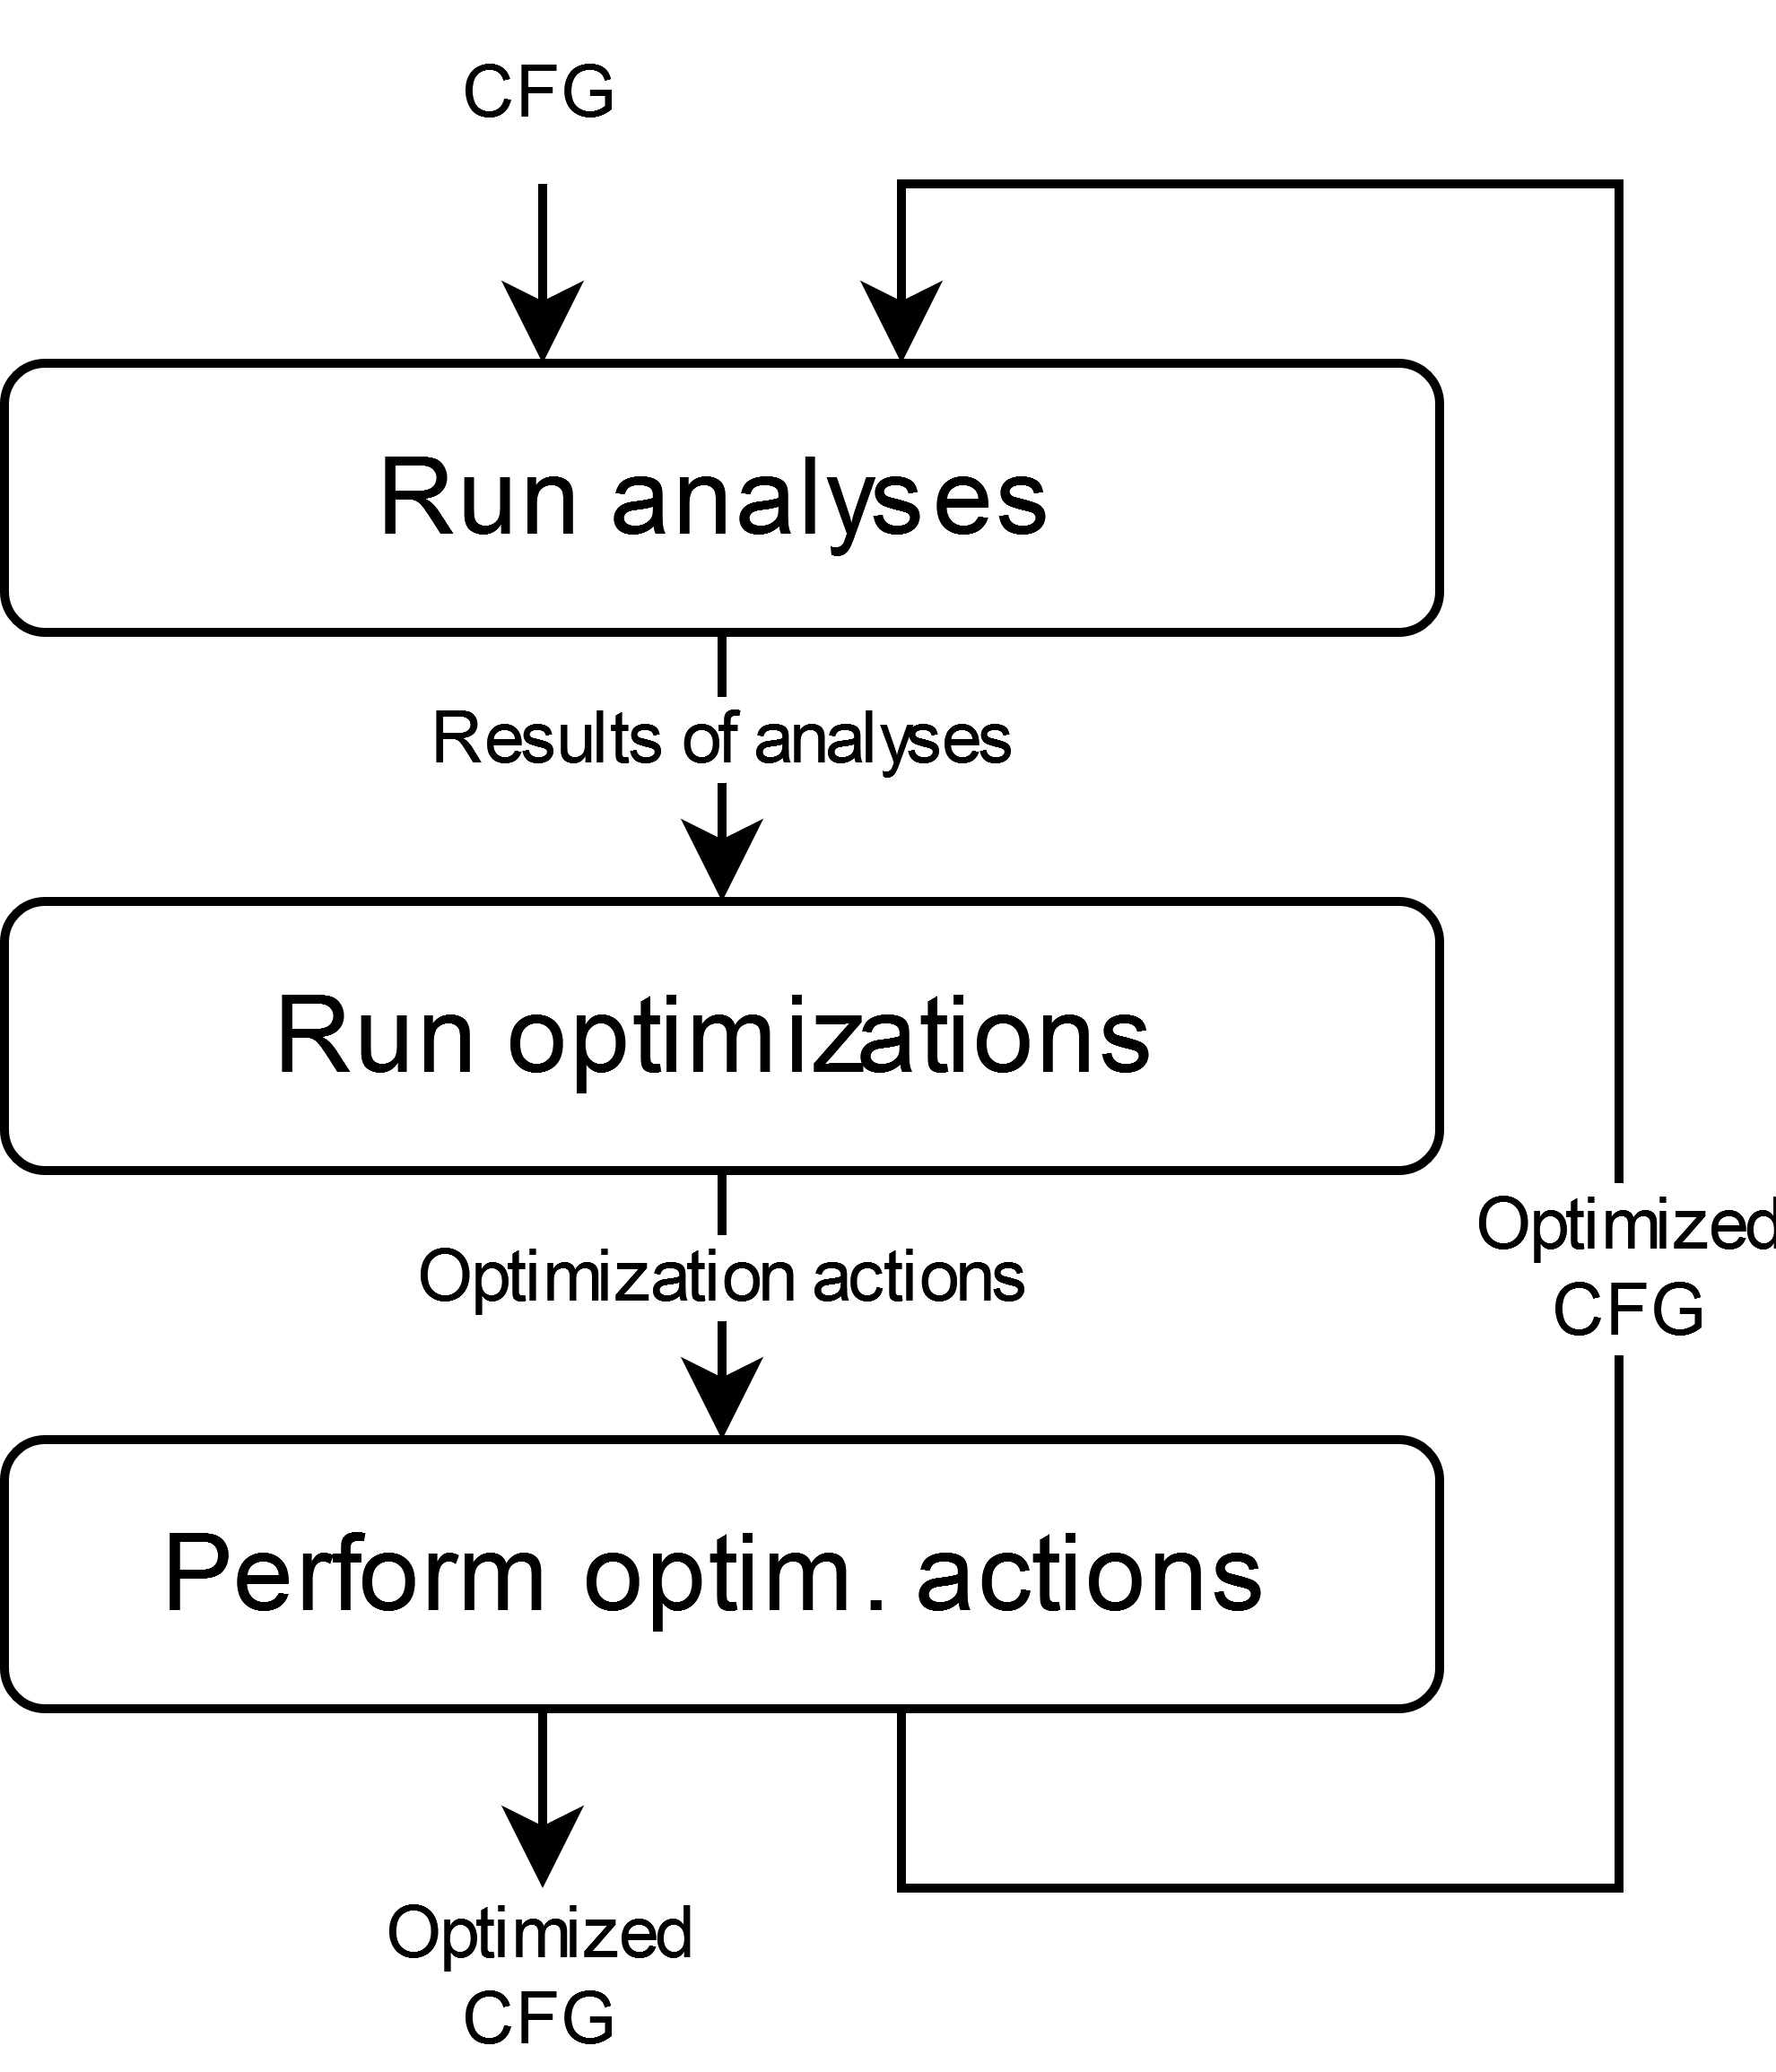
\includegraphics[height=5.4cm]{img/optimizing}
    \caption{An optimization process.}\label{fig:optimizing}
\end{figure}

So far, we have used the term \emph{optimization action} without giving proper examples and explanations. In the next few paragraphs, we will try to make up for it by covering each of the optimization actions supported by the optimizer.

\paragraph*{Deletion of a node} The node is removed from the CFG while keeping all of its edges. Edges from predecessors of the deleted node are reconnected to successors of the node. Similarly, edges to successors of the deleted node are reconnected to predecessors of the node.

\paragraph*{Connection of nodes} A new directed edge is created between two nodes.

\paragraph*{Disconnection of a node} The node is removed from the CFG together with all of its edges.

\paragraph*{Replacement of a node} The node is replaced with a different node.

\paragraph*{Prependition of a node} The node is prepended with a new node. The new node becomes the only predecessor of the node, and all of its previous predecessors are reconnected to the new node.

\paragraph*{Addition of a declaration} A new declaration of a variable is added.

\paragraph*{Deletion of a declaration} Declaration of a variable is removed.

\paragraph*{Change of a context} Context of the node is changed to a different one.

\paragraph*{} With examples of optimization actions out of the way, we will now move on to the introduction of optimizations used by the optimizer.

\subsection{Dead statement elimination}
The first optimization that will our optimizer use is the \emph{dead statement elimination}. This optimization utilizes the result of the live variable analysis to determine which statements (or, to be precise, which assignments) can be removed without affecting the program results.

Recall the CFG example from \autoref{fig:cfg}---the variable \texttt{y} is assigned to in the node \texttt{y = \{a: x * -10\}}, but the value is never read and is overwritten in the node \texttt{y = \{a: x\}}. Therefore, since the first assignment does not introduce any side-effect and has no effect on the program, we can safely get rid of it. This constraint is very important, statements that contain side-effect inducing expressions (like \texttt{input} or call of a function that contains \texttt{input} or \texttt{output}) cannot be eliminated, since that would change observable behaviour of the program. In case the Rhs of the assignment contains side-effect inducing expressions, we will replace the whole assignment with its Rhs. This way we get rid of the assignment while also not changing the observable behaviour of the program. 

The live variable analysis tells us which variables are live \emph{before} the given CFG node (cf. \autoref{ssec:live_var_analysis}). To decide whether the assignment can be eliminated, we have to check if the variable that is being assigned to is dead before every successor of the assignment node. If it is, the node containing the assignment can be safely deleted (or replaced if the assigned expression contains a side-effect).

\subsection{Dead code elimination}\label{ssec:dead_code_elim}
The goal of our version of the \emph{dead code elimination} will be eliminating dead branches of \emph{while}, \emph{do-while}, and \emph{if} statements. The branch is dead if it will never be executed for every possible input of the program. There are 4 cases where this happens:
\begin{enumerate}
    \item If-statement where the guard is a non-zero integer. In this case, the \emph{else} branch together with the guard can be safely eliminated.
    \item If-statement where the guard is an integer $0$. Here, the \emph{then} branch and the guard can be eliminated.
    \item While-statement where the guard is an integer $0$. In this case, the body of the while-loop and the guard can be eliminated.
    \item Do-while-statement where the guard is an integer $0$. Since the body of the loop will be executed only once, the guard can be eliminated and the branch is transformed into a simple sequence of nodes with one entry and one exit.
\end{enumerate}

At first glance it may seem unnecessary to eliminate code that would have never been executed in the first place, however by doing so we are shrinking program size (which is an optimization), but most importantly, this elimination can enable further optimizations. Take the program from \autoref{fig:dead_code_elim} as an example---by eliminating the \emph{else} branch, we got rid of all reads of the variable \texttt{y}, which then enables the dead statement elimination that will eliminate the assignment \texttt{y = 5}.

To perform this optimization we will simply scan the CFG for guards of \emph{if}, \emph{while}, and \emph{do-while} statements that evaluate to \texttt{true} or \texttt{false} and then perform the described eliminations by disconnecting entry and exit nodes of the eliminated branch. No analysis is required for this optimization.

\begin{figure}
	\centering
	\subfloat[Before.]{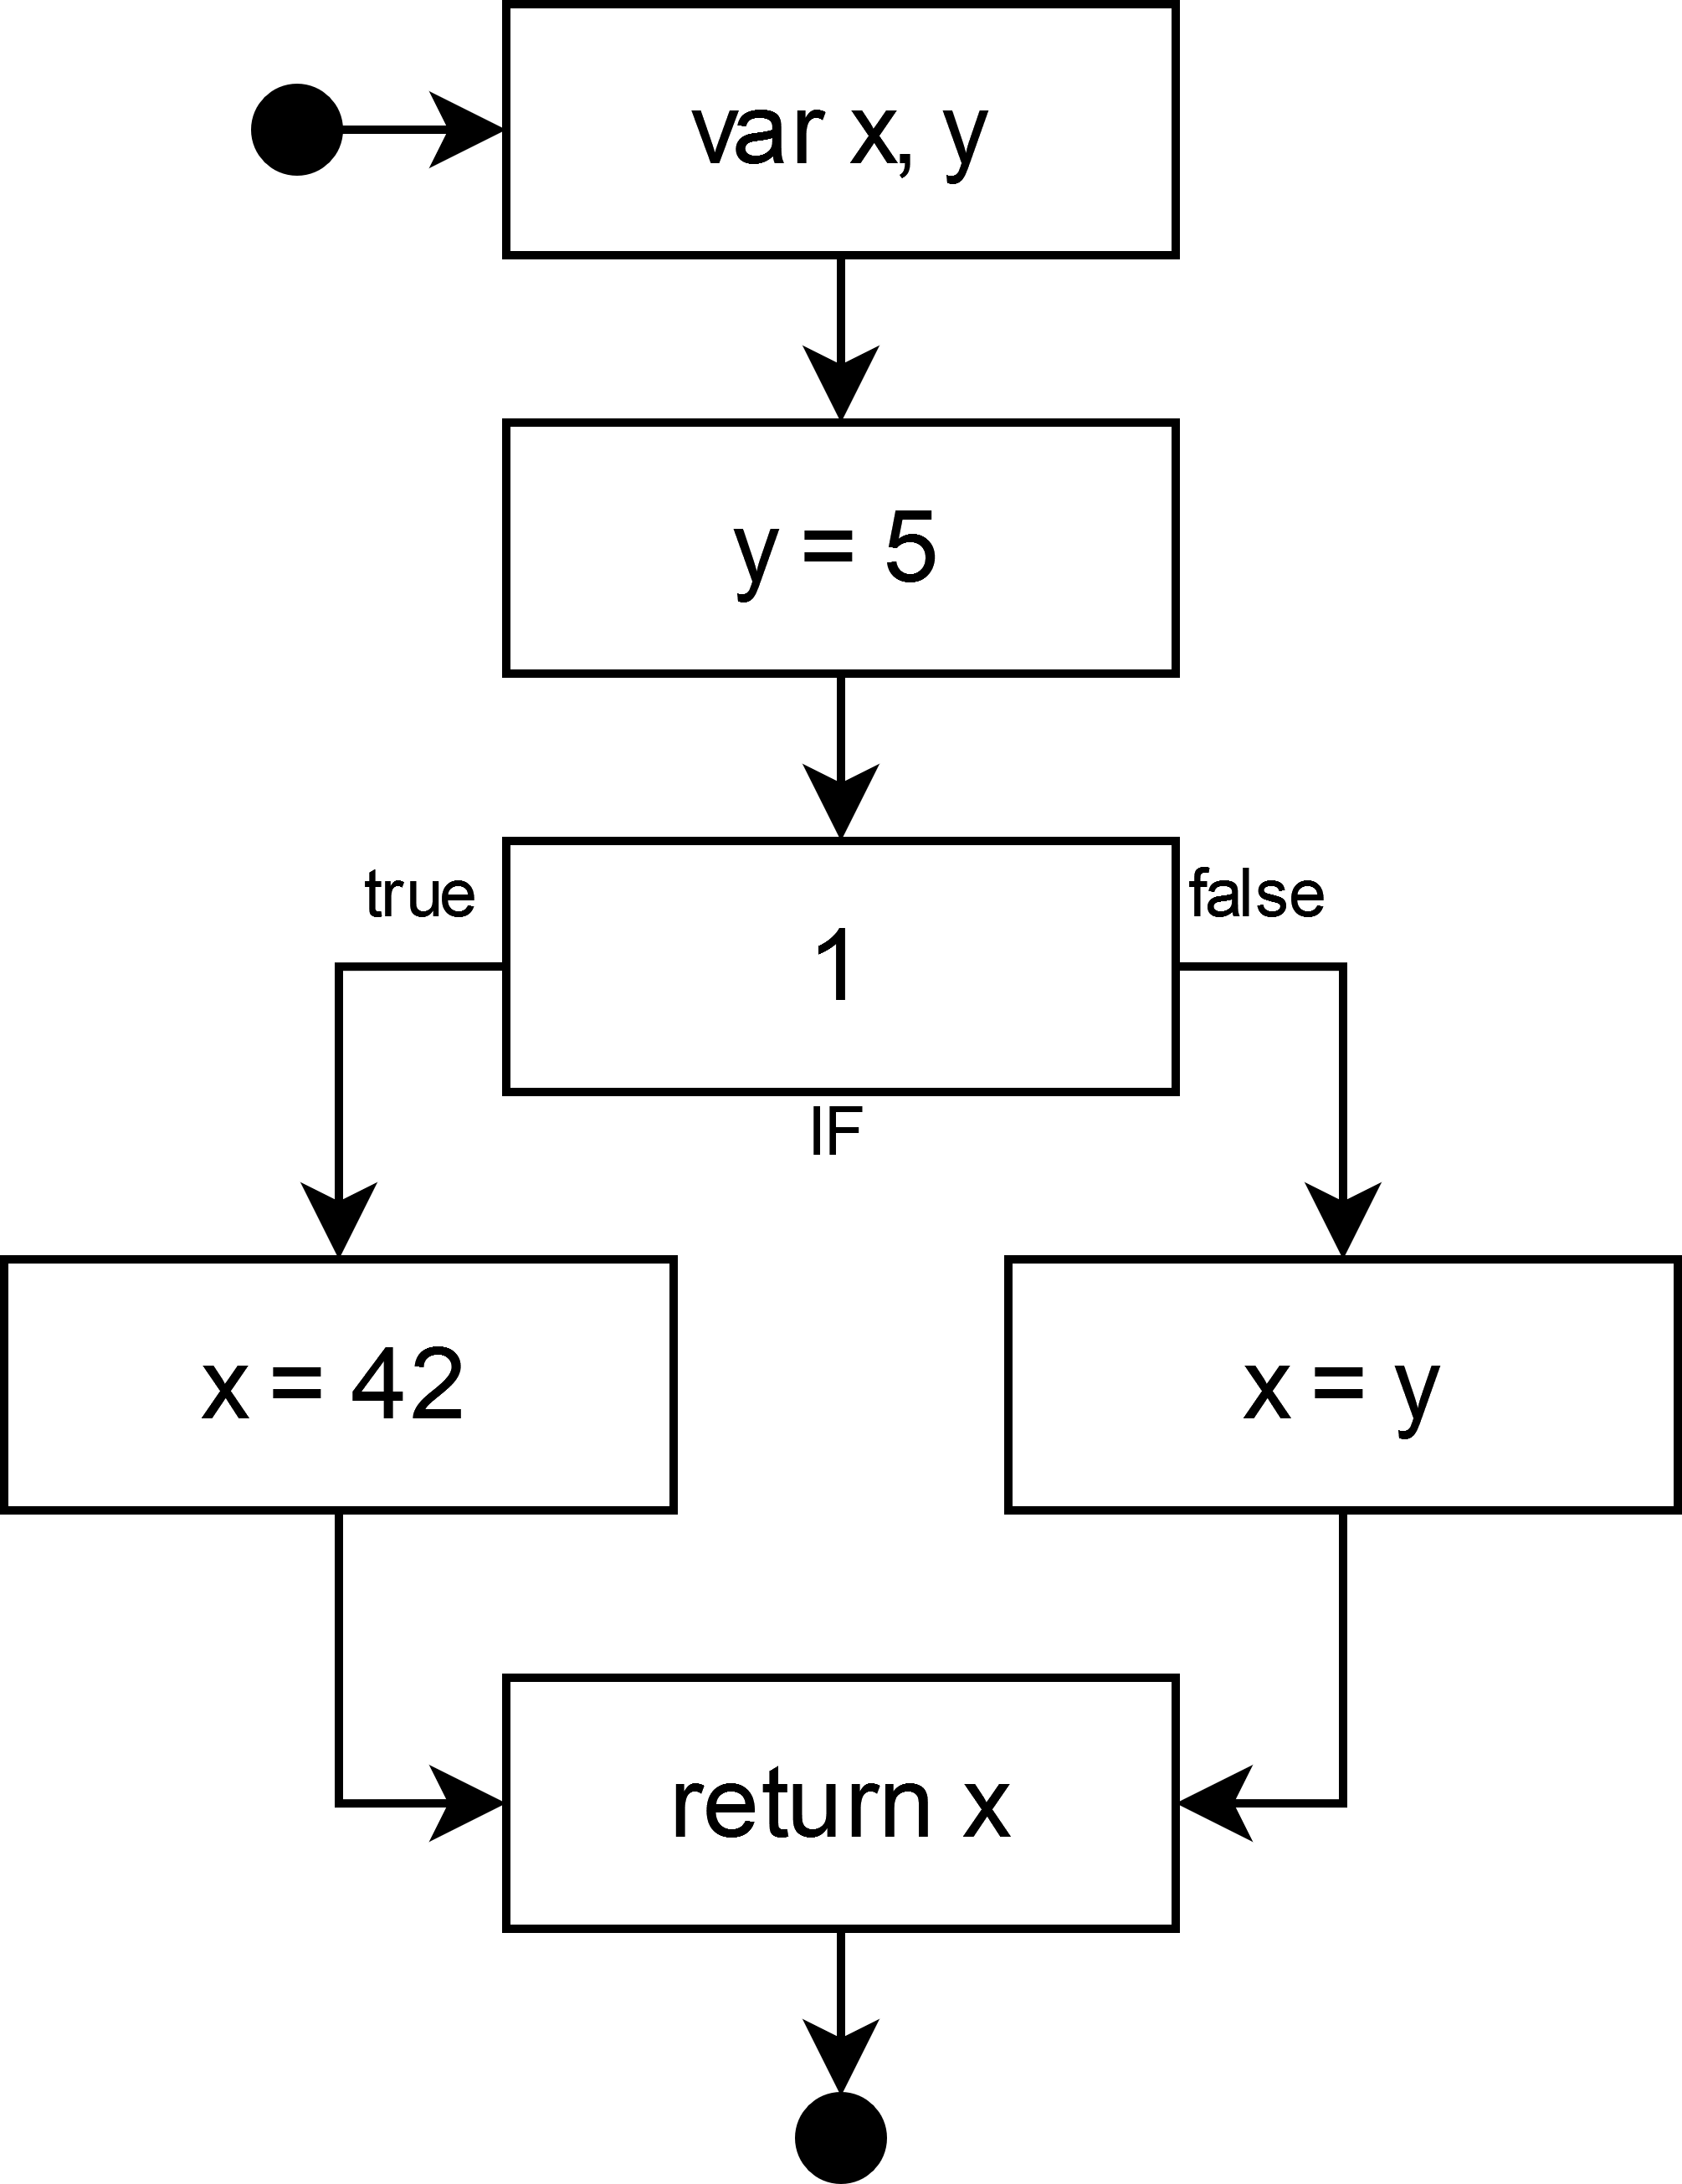
\includegraphics[width=5.05cm]{img/dead_code_before.png}}
	\hspace{1em}
	\subfloat[After.]{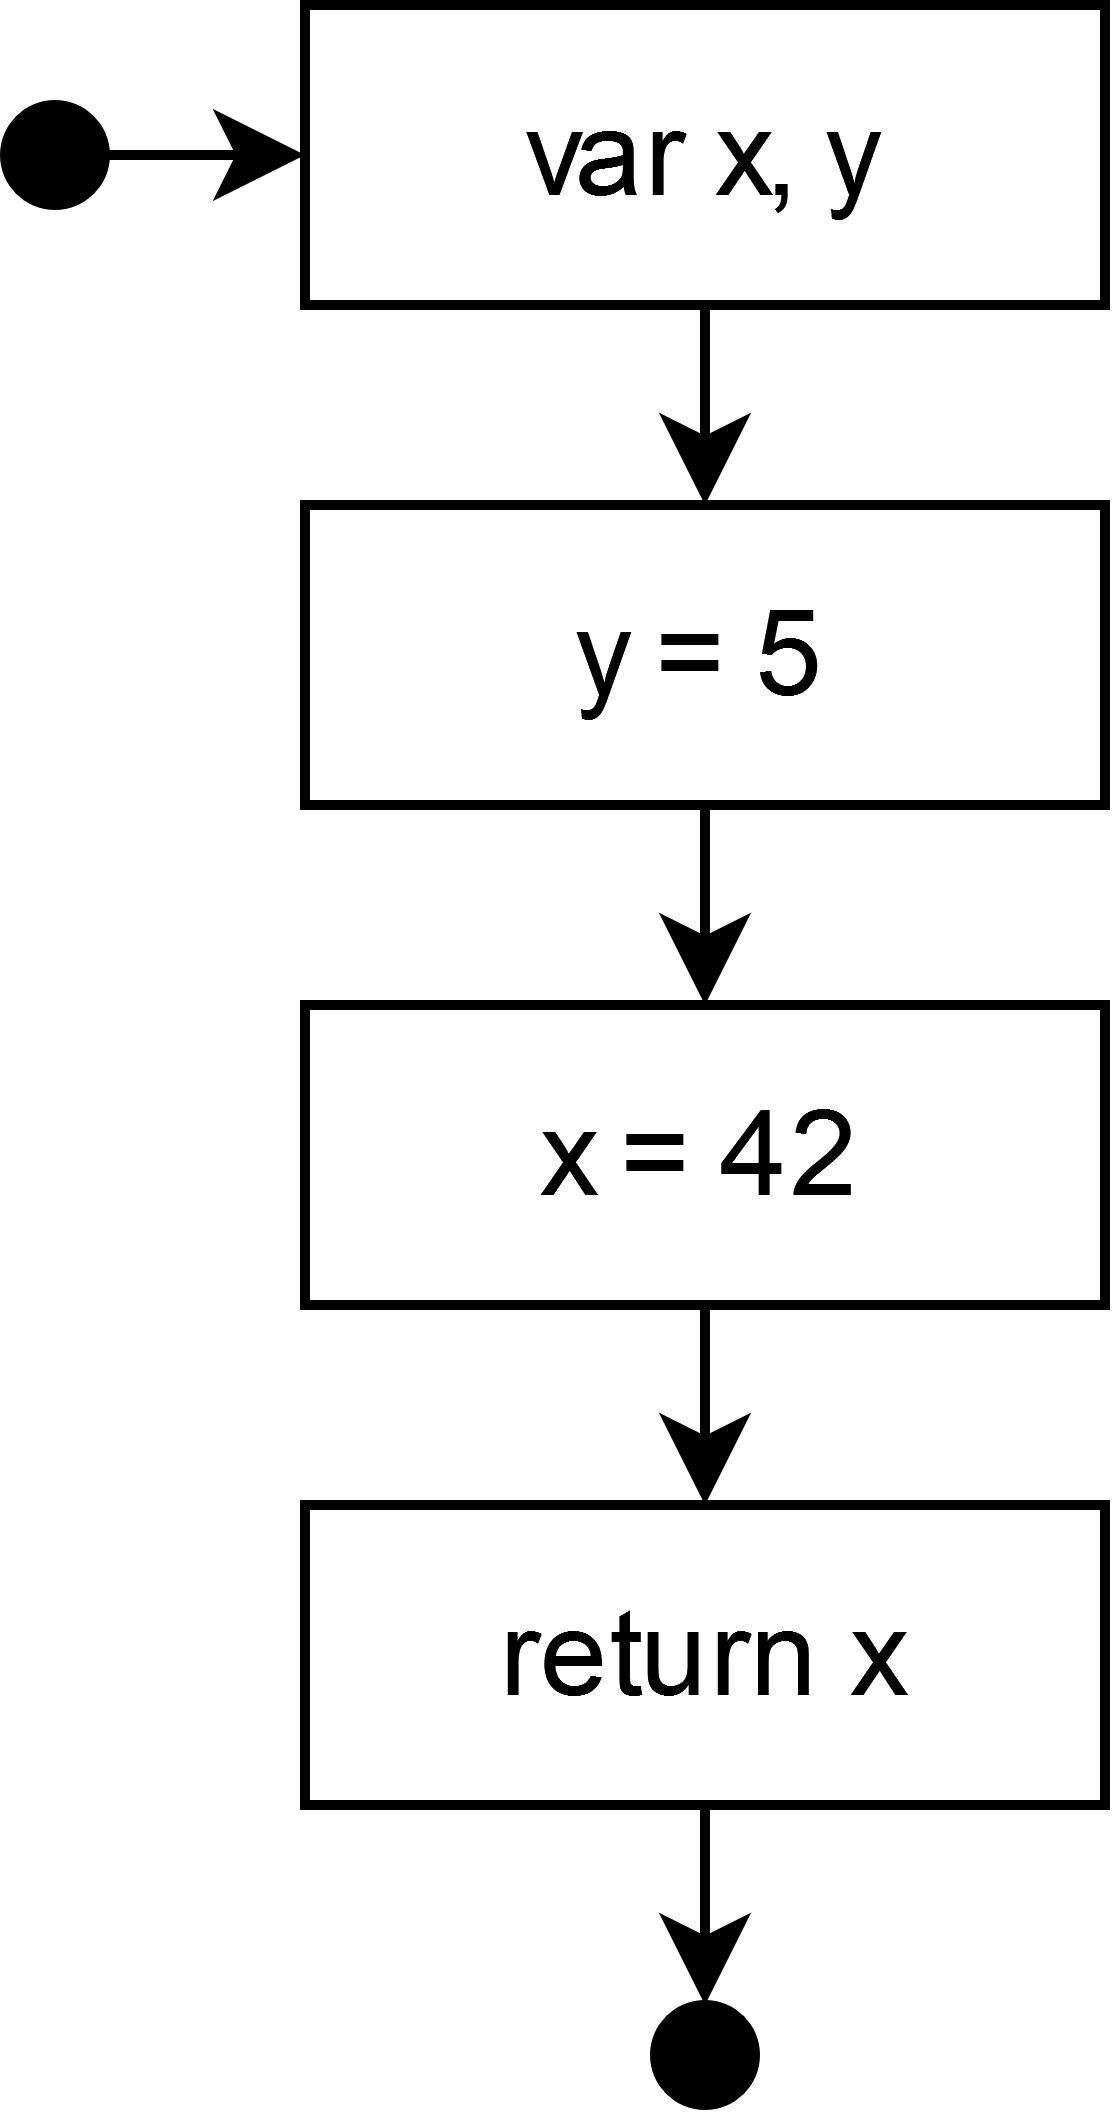
\includegraphics[width=2.8cm]{img/dead_code_after.png}}
	\caption{Example of dead code elimination.}
	\label{fig:dead_code_elim}
\end{figure}
\pagebreak

\subsection{Constant-based dead code elimination}
Previous optimization is a simple optimization that does not require any analysis. However, it can be improved by providing more information about the optimized program, e.g., by providing a result of the constant propagation analysis. Take the program from \autoref{lst:optimizable_program} as an example---after the first if-statement, the variable \texttt{x} will always evaluate to \texttt{true} (since both $5$ and $10$ are interpreted as \texttt{true}), therefore both the \emph{else} branch and the guard of the second if-statement can be safely eliminated.

\begin{listing}[H]
    \centering
	\inputminted[tabsize=2,breaklines,bgcolor=codebg,escapeinside=||]{python}{snippets/optimizable_program.m}
	\caption{An optimizable program.}
	\label{lst:optimizable_program}
\end{listing}

The \emph{constant-based dead code elimination} is an improved version of the dead code elimination. It utilizes a result of the constant propagation analysis to decide which guards of \emph{if}, \emph{while}, and \emph{do-while} evaluate to \texttt{true} or \texttt{false} and then performs eliminations described in \autoref{ssec:dead_code_elim}. In addition, it also performs optimization in the case where the guard of while-statement evaluates to \texttt{true} during the first evaluation of the guard. This means that the body of the loop will get executed at least once. In this case, the while-statement can be transformed into a do-while-statement with the same guard and body.

\subsection{Sign-based dead code elimination}
The \emph{sign-based dead code elimination} is another example of an improved dead code elimination. It performs the same kind of optimizations as the constant-based dead code elimination, but it utilizes a result of the sign analysis instead.

\subsection{Unused variable elimination}
Any declaration of a variable that is never used in the function it was declared in can be safely eliminated. By doing so, we are shrinking the space allocated for local variables on a stack frame (recall storage organization of an x86 target machine discussed in \autoref{ssec:storage_org}). This optimization is called \emph{unused variable elimination}.

To decide whether a variable is unused, we will scan the CFG for usages of the variable. If no usages are found, we will remove the declaration of the variable. No analysis is required for this scan.

\subsection{Constant folding}
The \emph{constant folding} optimization is used to optimize binary operations using a set of rewrite-rules which consist of application of algebraic identities and evaluation of constant expressions. The rules we will be using are listed below (algebraic identities are taken from \cite[Chap. 8.5.4]{dragonbook}):

\begin{align*}
    \texttt{0 + Expr} &\longrightarrow \texttt{Expr}\\
    \texttt{Expr + 0} &\longrightarrow \texttt{Expr}\\
    \texttt{Expr - 0} &\longrightarrow \texttt{Expr}\\
    \texttt{Id - Id} &\longrightarrow \texttt{0}\\
    \texttt{Id * 0} &\longrightarrow \texttt{0}\\
    \texttt{0 * Id} &\longrightarrow \texttt{0}\\
    \texttt{Expr * 1} &\longrightarrow \texttt{Expr}\\
    \texttt{1 * Expr} &\longrightarrow \texttt{Expr}\\
    \texttt{Expr / 1} &\longrightarrow \texttt{Expr}\\
    \texttt{Int op Int} &\longrightarrow \texttt{$eval(\texttt{Int op Int})$}
\end{align*}

It may seem like some rules for division (e.g., $\texttt{0 / Expr} \longrightarrow \texttt{0}$) are missing, however those cannot be eliminated because of possible division by zero. By rewriting such division, we would change observable behaviour of the program. The same applies to rules such as $\texttt{0 * Expr} \longrightarrow \texttt{0}$, since the \texttt{Expr} itself can contain division by zero.

We will perform this optimization by scanning the CFG for nodes containing binary operations which match the listed rewrite-rules. The nodes are then replaced based on the given rewrite-rules.

\subsection{Sign folding}
The \emph{sign folding} is very similar to constant folding, the only difference is that the rewrite-rules of sign folding utilize the result of the sign analysis. The optimization is applied on binary operations \emph{equal} and \emph{greater-than}, and the rewrite-rules for each of them are listed in \autoref{tab:rewrite_rules}. Note that in microC \texttt{true} and \texttt{false} are represented by $1$ and $0$, respectively. Optimization is also applied to identifiers with a sign \texttt{0}, which are replaced with a constant $0$.

\begin{table}
\begin{minipage}{.5\linewidth}
    \centering
    \begin{tabular}{|c||c|c|c|}
    \hline
    \texttt{==} & \texttt{+} & \texttt{0} & \texttt{-}\\
    \hline
    \hline
    \texttt{+} & -- & \texttt{false} & \texttt{false}\\
    \hline
    \texttt{0} & \texttt{false} & \texttt{true} & \texttt{false}\\
    \hline
    \texttt{-} & \texttt{false} & \texttt{false} & --\\
    \hline
    \end{tabular}
\end{minipage}%
\begin{minipage}{.5\linewidth}
    \begin{tabular}{|c||c|c|c|}
    \hline
    \texttt{>} & \texttt{+} & \texttt{0} & \texttt{-}\\
    \hline
    \hline
    \texttt{+} & -- & \texttt{true} & \texttt{true}\\
    \hline
    \texttt{0} & \texttt{false} & \texttt{false} & \texttt{true}\\
    \hline
    \texttt{-} & \texttt{false} & \texttt{false} & --\\
    \hline
    \end{tabular}
\end{minipage}%
\caption[The rewrite-rules for binary operations \emph{equal} and \emph{greater-than}.]{The rewrite-rules for binary operations \emph{equal} and \emph{greater-than}. Rows and columns represent Lhs and Rhs operands, respectively.}\label{tab:rewrite_rules}
\end{table}

Similarly to constant folding, the optimization is performed by scanning the CFG for nodes containing binary operations and using the result of sign analysis to determine signs of operands of the binary operation. If signs match the listed rewrite-rules, the node is then replaced based on the given rule.

\subsection{Constant propagation}
The goal of the \emph{constant propagation} is to substitute variables with constant values (assuming that the constant values are known at compile time) using the result of the constant propagation analysis. This leads to a more optimal program while also possibly enabling further optimizations like constant folding. Recall the CFG example from \autoref{fig:cfg}---if we use the result of a constant propagation analysis from \autoref{ssec:constant_prop_analysis}, we can safely replace the variable \texttt{x} in the node \texttt{y=\{a:x*-10\}} with a constant value $5$.

The constant propagation analysis tells us constant values of variables \emph{after} the given CFG node (recall \autoref{ssec:constant_prop_analysis}). To decide whether a variable in a CFG node can be replaced, we have to check if the variable has constant value in the predecessors of the node. If it has, we can replace every occurrence of the variable in the node with that constant value.

\subsection{Common subexpression elimination}
The \emph{common subexpression elimination} gets rid of non-trivial expressions that have been already calculated by the time the flow control reaches them. Results of such expressions are stored in temporary variables, which are then used instead of the redundant expressions \cite[Chap. 9.5.1]{dragonbook}. This is done by utilizing the result of an available expression analysis. Take the program from \autoref{fig:common_subexp_elim} as an example---expression \texttt{x / 5} is already available at the return node, therefore we can introduce a new variable \texttt{t1} in which we will store this expression and eliminate its every other occurrence.

\begin{figure}
	\centering
	\subfloat[Before.]{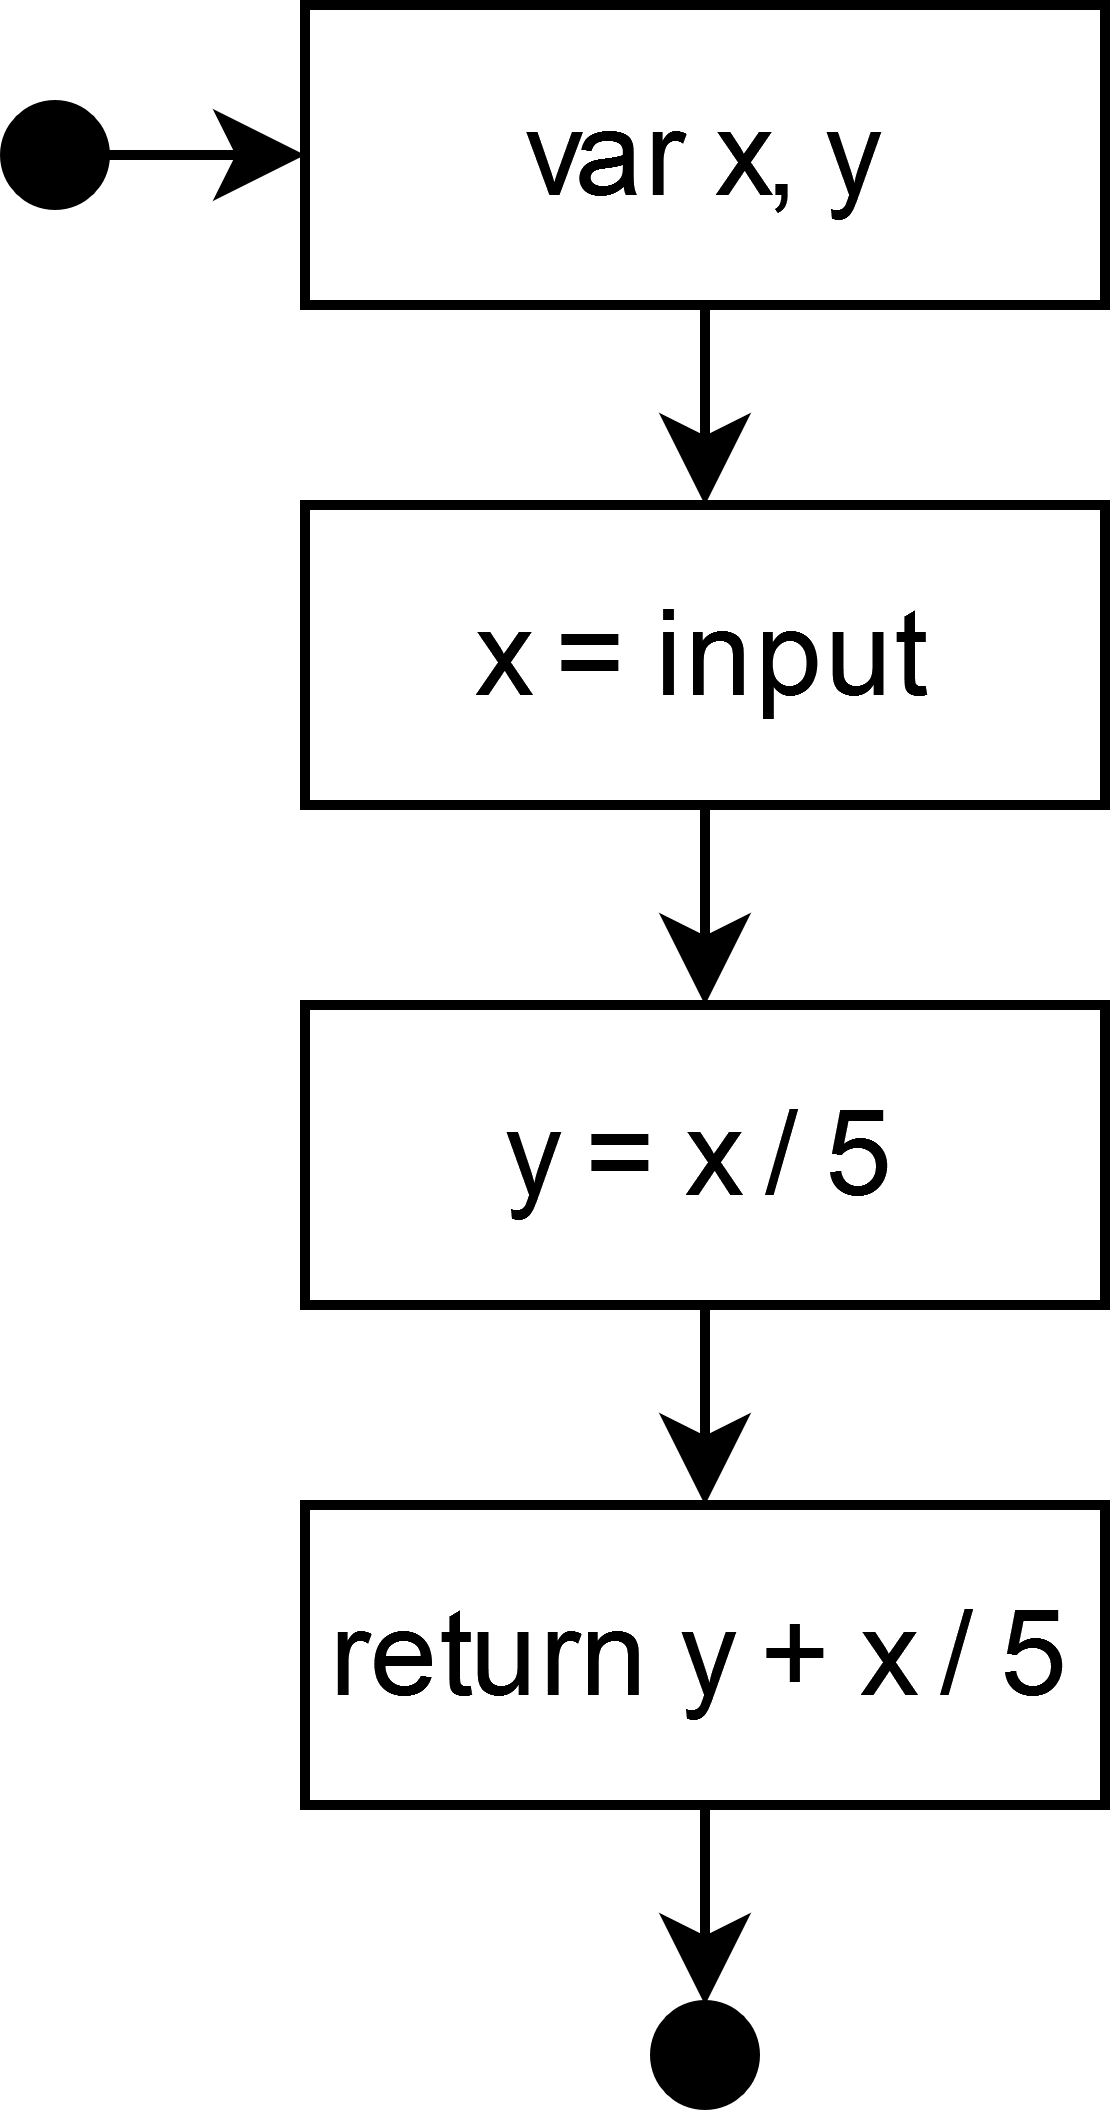
\includegraphics[width=2.8cm]{img/cse_before.png}}
	\hspace{1em}
	\subfloat[After.]{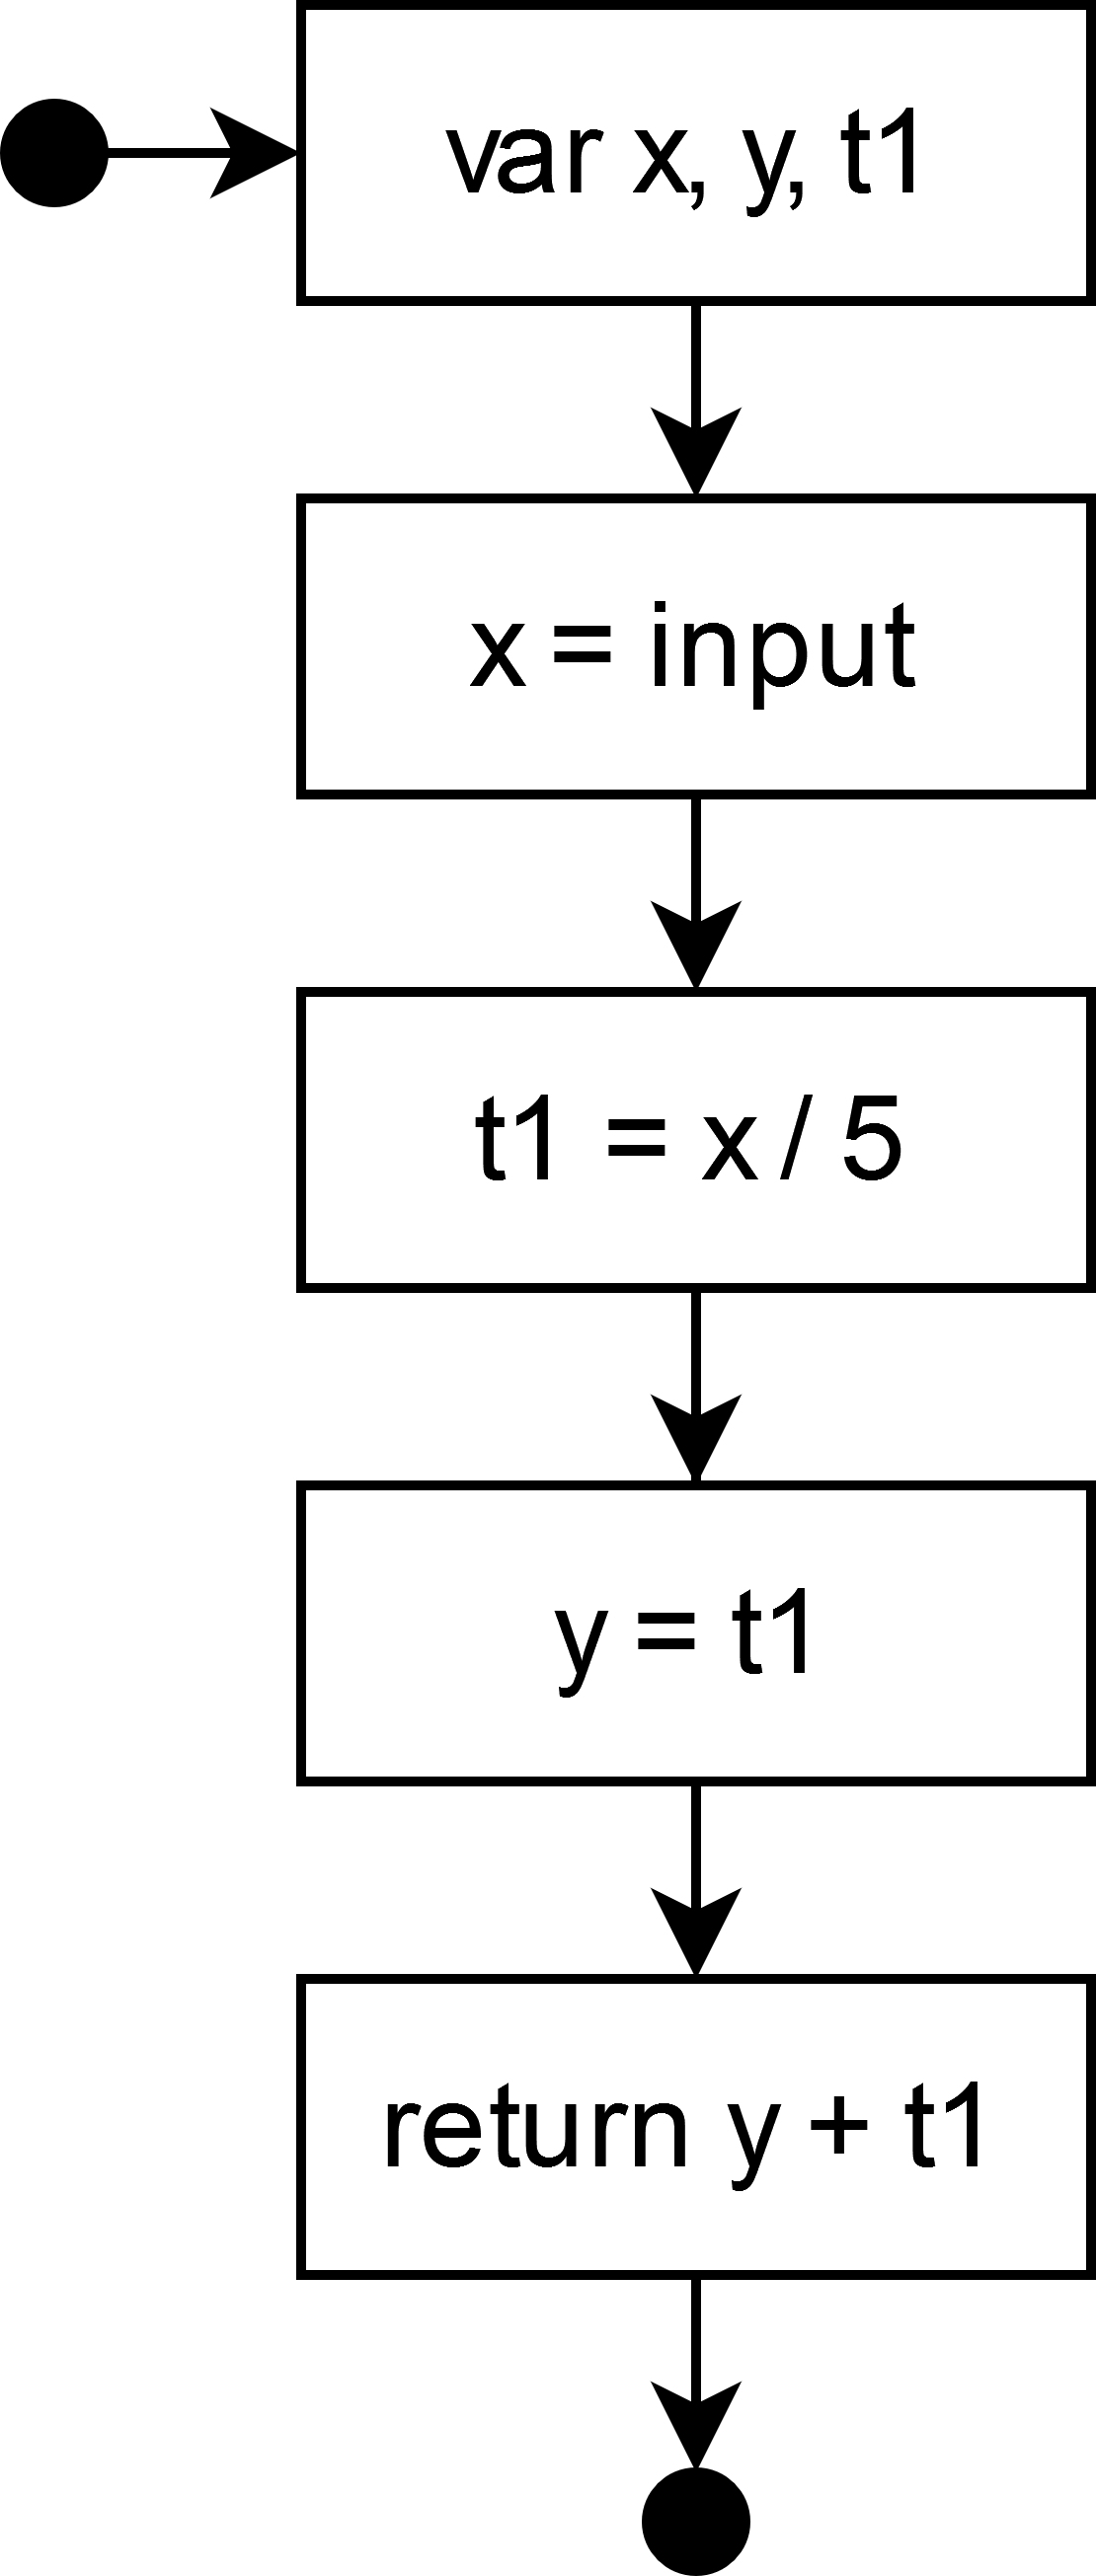
\includegraphics[width=2.8cm]{img/cse_after.png}}
	\caption{Example of common subexpression elimination.}
	\label{fig:common_subexp_elim}
\end{figure}

We will perform this optimization by finding an available expression that is used in the program more than once. Then we will create a new CFG node that stores this expression in a temporary variable and prepend the node to a node that contains the first occurrence of the expression. Every occurrence of the expression (except for the newly created node) can then be replaced with the new temporary variable (assuming that the expression is available at the given point).

\subsection{Summary of the middleend}
In this section, we have covered design of every component of the middleend. If we put the components together (as illustrated in \autoref{fig:microc_middleend}), we will get a middleend that takes an AST from a frontend, constructs a CFG from it, performs various optimizations on the CFG, and produces an optimized CFG together with results of CFG analyses. These results will be further utilized in the backend (e.g., result of type analysis is required for code generation of x86IR, which we will discuss in the following section).

\begin{figure}
    \centering
    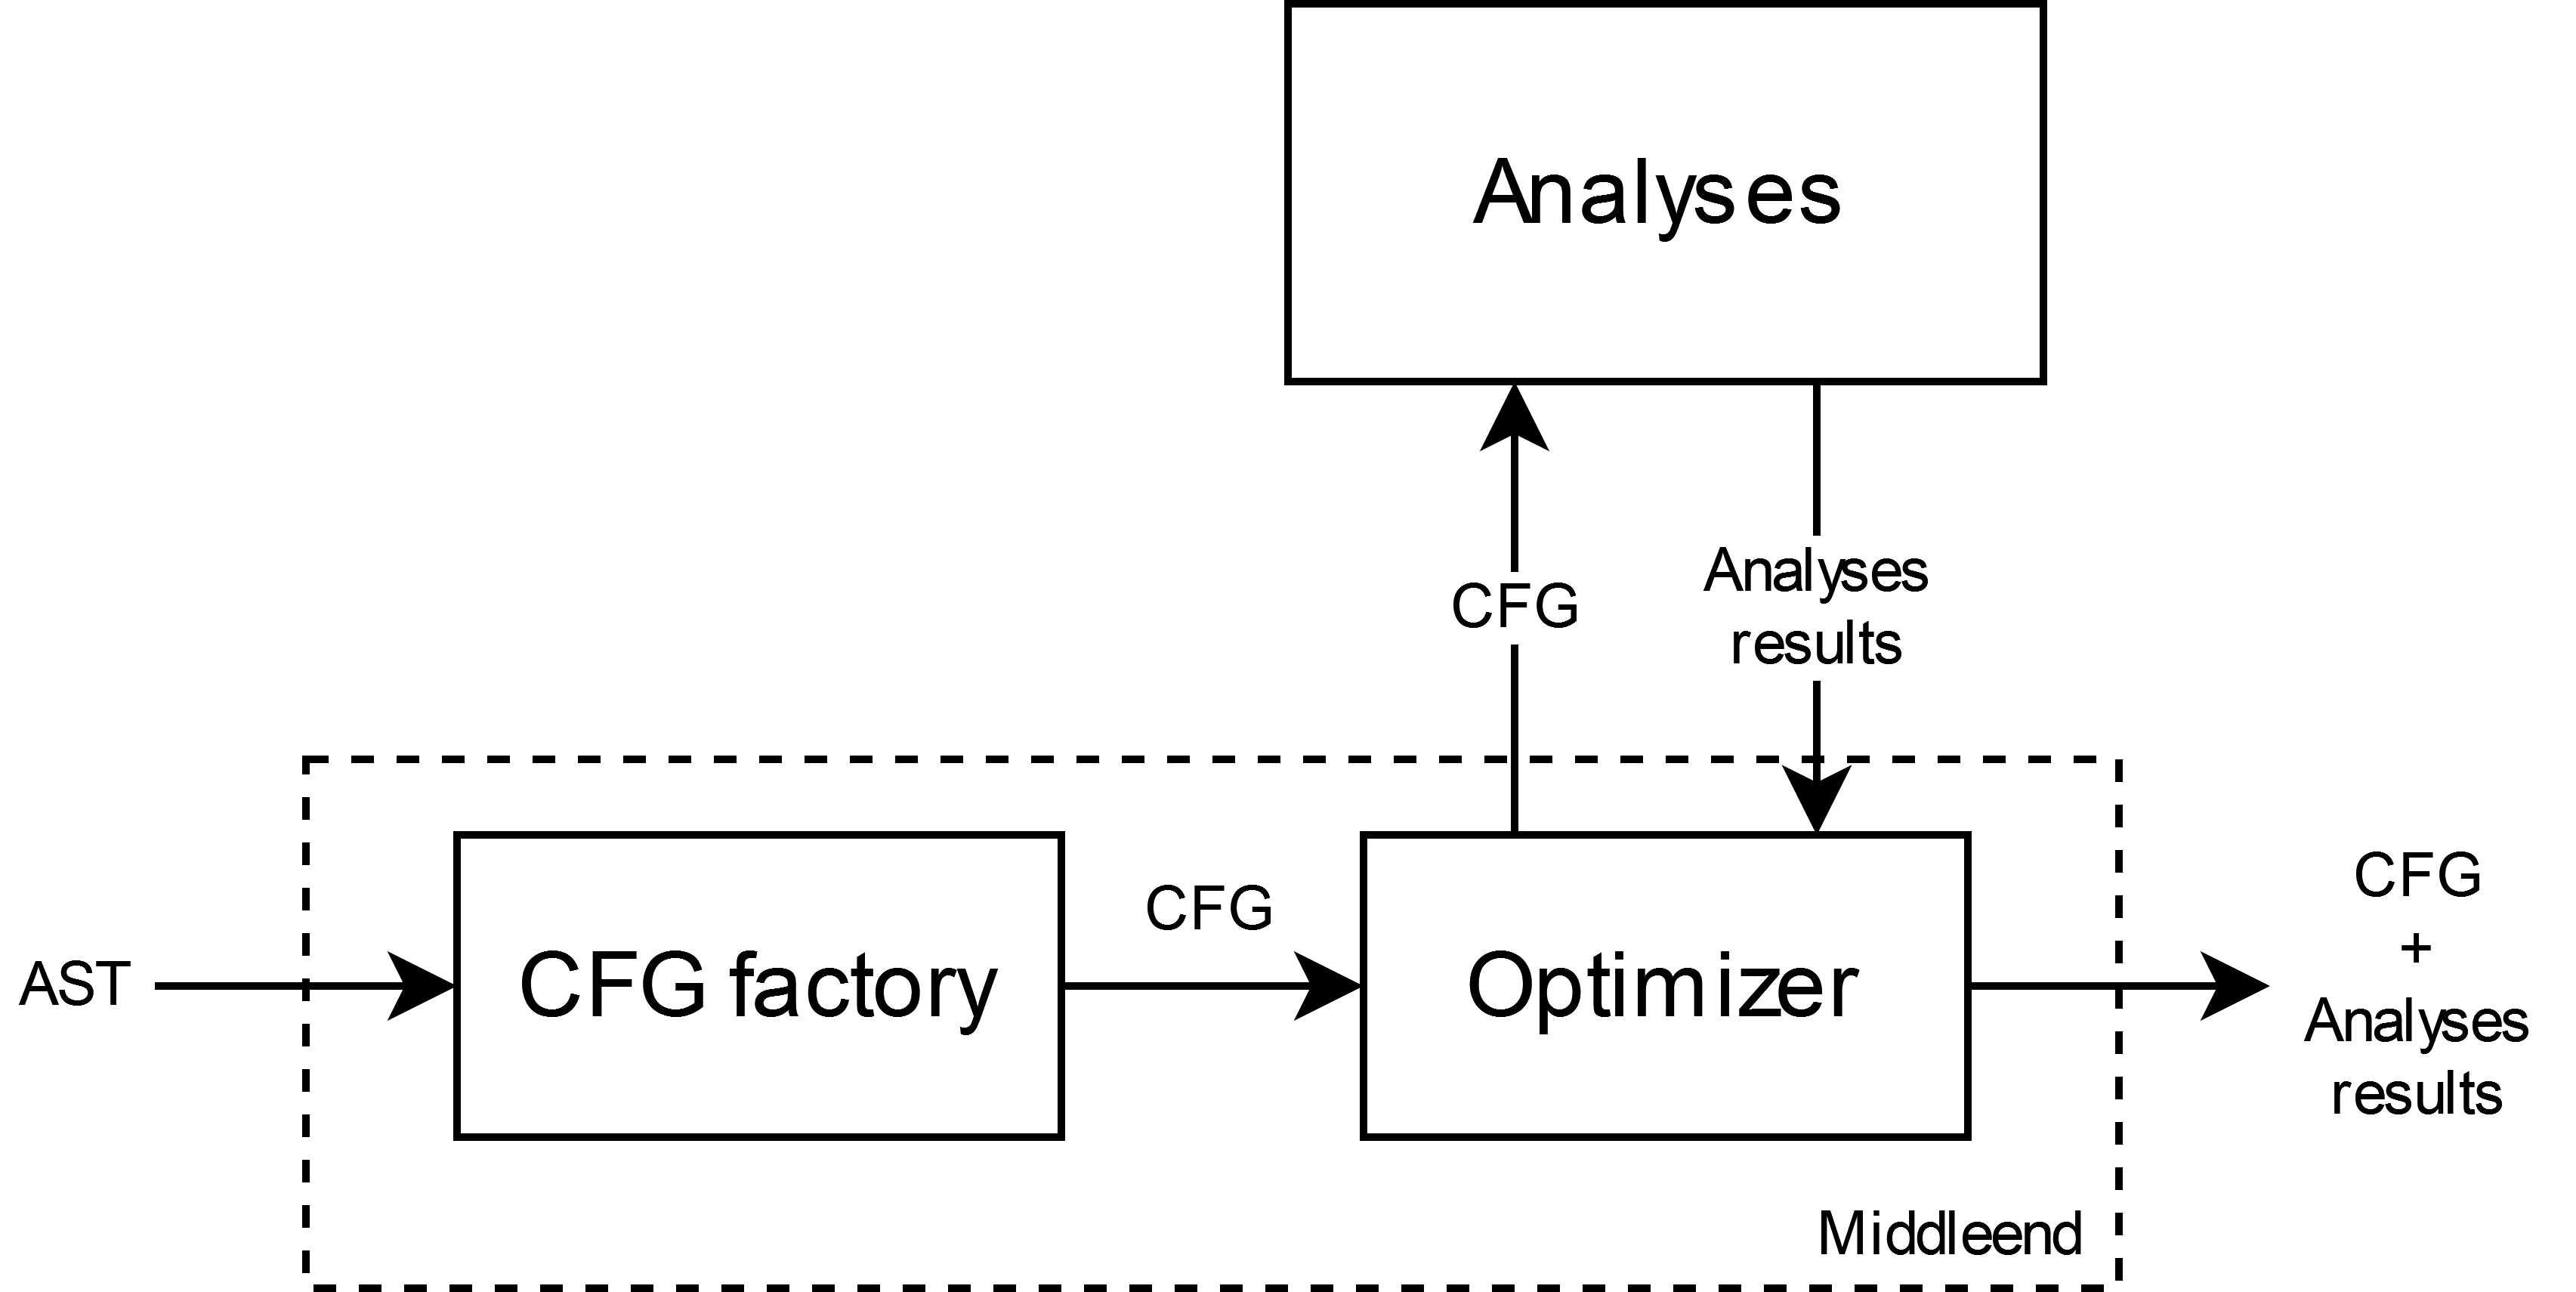
\includegraphics[width=11cm]{img/microc_middleend.png}
    \caption{The middleend of the microC compiler.}\label{fig:microc_middleend}
\end{figure}

\section{The backend}
The responsibility of our compiler's backend will be to use the CFG provided by the middleend to generate an x86 program, which may be further optimized by machine-dependent optimizations. These optimizations typically exploit peculiarities of the target architecture \cite[Chap. 1.0]{comp_design} (in our case, the x86-64 architecture). In the following subsection, we introduce yet another IR to help us map CFG IR to x86-64 instruction set.

\subsection{x86IR}\label{ssec:x86ir}
The \autoref{ssec:cfg_as_ir} covered CFG IR, which was conveniently designed for various types of analysis and optimizations. One of the nice properties of the CFG IR was the independence from any particular source or target language. However, precisely this independence makes the CFG IR not well suited for a direct compilation into our target language, x86-64 assembly. To tackle this issue, we will have to introduce a lower level IR that will serve as an intermediate step between CFG IR and x86-64 assembly. We will refer to this IR as an \emph{x86IR}.

Generally, an assembly-language program is a form of a linear code. It consists of instructions that execute in their order of appearance \cite[Chap. 5.3]{eng_comp}. The x86IR is a linear IR that resembles this structure as much as possible. Abstract syntax of the x86IR is defined in \autoref{lst:x86IR}.

\paragraph*{Instruction} The x86IR instruction set takes inspiration from the LLVM instruction set \cite[Instruction Reference]{llvm} and consists of a total of 17 instructions (see \autoref{sec:x86IR_instr_set} for a detailed overview of the instruction set). These instructions can be divided into 4 categories:
\begin{itemize}
    \item \emph{Terminator instructions}---these instructions typically yield no value and their sole purpose is to produce control flow at the end of a basic block. Examples: \emph{Return}, \emph{CondJump}, and \emph{Jump}.
    \item \emph{Memory instructions}---these instructions allow not only to allocate, read and write memory, but also to retrieve or calculate memory addresses of values. Examples: \emph{Alloc}, \emph{FunAlloc}, \emph{HeapAlloc}, \emph{ArgAddr}, \emph{GetAddr}, \emph{GetAddrOffset}, \emph{Load}, and \emph{Store}.
    \item \emph{I/O instructions}---instructions that handle I/O operations. Examples: \emph{LoadInput} and \emph{Print}.
    \item \emph{Other instructions}---instructions that don't fit in any of the previous categories. Examples: \emph{LoadImm}, \emph{LoadComposed}, \emph{BinOp}, and \emph{Call}.
\end{itemize}
Even though every instruction has different properties and operands, each of them shares common fundamental properties---\emph{location} and \emph{type}.

The location of an instruction is information about its origin in a microC source code (line and column). It is used in error reports to direct the user to the source of the error.

The type of instruction is important information that will come handy for a compilation from x86IR to x86 assembly. It will tell us how to handle the result of an instruction (e.g., how to store it in registers or memory) or the byte-size of the result, which will be used to calculate the total byte-size of a stack frame. There are 4 types in total:
\begin{itemize}
    \item \emph{VoidType}---type of an instruction that yields no value, therefore the byte-size of the instruction's result is 0.
    \item \emph{SimpleType}---type of an instruction that returns a non-composed simple value, like an integer or a function. Byte-size of the type is 8 bytes\footnote{Even though we will be using 32-bit integers, their size on the stack will be 64 bits, since the x86-64 instructions \texttt{push} and \texttt{pop} allow only 64-bit operands \cite[Chap. 9.2]{x86_assembly}\cite{so_push}.} (equal to the size of an x86-64 register).
    \item \emph{ComposedType}---type of an instruction that returns a value that is composed of one or more values (e.g., Record). Its byte-size is a sum of all types of which it consists.
    \item \emph{PointType}---type of an instruction that returns an address of some value (equivalent to a pointer in the C programming language). Byte-size of the type is equal to the size of an address (8 bytes).
\end{itemize}

\paragraph*{Basic block} A \emph{basic block} is a named sequence of instructions that has single entry and single exit point. The exit point (i.e., the last instruction) of a basic block is a terminator instruction (such as jump or function return). Each basic block contains exactly one terminator instruction.

\paragraph*{Function} Program functions consists of a name of the function, number of parameters, and most importantly a sequence of basic blocks. A function has a single entry point---the first basic block in the basic block sequence.

\paragraph*{The x86IR program} Finally, the program in x86IR is represented by a simple list of one or more functions. One of these function is designated as an entry function (usually the one with the name \emph{main}), which means the function serves as the starting point for program execution.

\subsection{Code generation of x86IR}\label{ssec:x86ir_gen}
Now that we are familiar with the x86IR, we can move on to designing a first component of the backend---\emph{CFG Compiler}, which will transform CFG IR into x86IR. MicroC program is in CFG represented as a set of smaller function CFGs. We will try to map each of these function CFGs into an x86IR \emph{function} by compiling each of its nodes. Since the CFG introduced in the NI-APR course defines 3 types of nodes (\emph{CfgFunEntryNode}, \emph{CfgFunExitNode}, and \emph{CfgStmtNode}), in the next few paragraphs we will cover how to compile each of these types.

\paragraph*{CfgFunEntryNode} As the name suggest, this node represents a function entry. We will initialize a new \emph{function} with an empty \emph{basic block}. Then we will emit \emph{ArgAddr} instruction for every parameter of the compiled function. Then we continue by compiling the next successor of the node (there is always only one successor).

\paragraph*{CfgFunExitNode} Once again, the name is self-explanatory---the node represents a function exit. We will finalize the \emph{function} we initialized in the \emph{CfgFunEntryNode} and since this is the last node of the function CFG, the compilation of the function ends here and we move to the next function.

\paragraph*{CfgStmtNode} This node represents a program statement. The way we will compile this node depends on its context (recall \autoref{ssec:cfg_as_ir}), which can be one of the following 4 types: \emph{Basic Context}, \emph{If Context}, \emph{While Context}, and \emph{Do-While Context}.

The most straight-forward is a node with \emph{Basic Context}. Since this node does not introduce any branching, we will simply compile the program statement and then continue by compiling the next successor of the node.

Nodes with \emph{If Context} are a little more complicated, since they introduce branching. First, we will compile the guard of the if-statement. Then we will create 3 empty \emph{basic blocks} which we will refer to as \emph{then}, \emph{else}, and \emph{finally}. After that we will emit \emph{CondJump} instruction which will based on the evaluated value of the guard jump either to \emph{then} or \emph{else} block. Now we will “enter” the \emph{then} block, compile the entire then-branch, and lastly emit \emph{Jump} instruction that will jump to the \emph{finally} block. The same process is repeated for the \emph{else} block and else-branch. Finally, we will enter the block \emph{finally} and continue with a compilation of a node, that comes first after the whole if-statement. For an illustration of a result of this process, see \autoref{fig:x86ir_if}.

Another type of node is a node with \emph{While Context}, which also introduces branching. Similarly to the previous context, we will create 3 empty \emph{basic blocks} which we will refer to as \emph{guard}, \emph{body}, and \emph{finally}. First we will emit \emph{Jump} instruction that will jump to the \emph{guard} block, then enter the \emph{guard} block, compile the guard of the while-statement, and lastly emit \emph{CondJump} instruction which will based on the evaluated value of the guard jump either to \emph{body} or \emph{finally} block. Then we will enter the \emph{body} block, compile the entire body-branch of the while-statement, and lastly emit \emph{Jump} instruction that will jump back to the \emph{guard} block. As a last step, we will enter the block \emph{finally} and continue with a compilation of a node, that comes first after the whole while-statement. For an illustration of a result of this process, see \autoref{fig:x86ir_while}.

The last type of node is a node with \emph{Do-While Context}. Again, we will create 3 empty \emph{basic blocks} which we will refer to as \emph{body}, \emph{guard}, and \emph{finally}. First we will emit \emph{Jump} instruction that will jump to the \emph{body} block, then enter the \emph{body} block, compile the body of the do-while-statement, and lastly emit \emph{Jump} instruction that will jump to the \emph{guard} block. Then we enter the \emph{guard} block, compile the guard of the do-while-statement, and lastly emit the \emph{CondJump} instruction which will based on the evaluated value of the guard jump either to \emph{body} or \emph{finally} block. As a last step, we enter the block \emph{finally} and continue with the compilation of a node, that comes first after the whole do-while-statement.

\paragraph*{} This concludes compilation of a CFG node into x86IR. The compilation of statements and expressions in those nodes is, for the most part, straight-forward---first we will compile operands of a statement/expression and then we compile the statement/expression itself. Therefore, it won't be discussed further. The only exception to this is compilation of a field access, which we will cover in the next and last part of this subsection.

\paragraph*{Field access} In a microC code, fields of a record are accessed using field names. However, the x86IR was designed to be more low-level and closer to the x86-64 assembly, therefore it has no concept of “field names”. In memory, a record is stored as a sequence of members (similarly to a struct type in C language \cite{c_struct} or structure type in LLVM \cite[Structure Type]{llvm}), so it only makes sense to access the members of a record by an offset (of bytes) from the address of the record (which will be the first member of the record). The size of the offset depends on the types (and their byte-sizes) of the record's members, which can be inferred by utilizing the result of a type analysis.

Take record \texttt{\{a:0, b:\{c:1, d:2\}\}} as an example\footnote{Officially, the microC language does not support nested records \cite[Records]{microc}, however in case this changes in the future, our compiler will support nested fields.}---to access the field \texttt{.b}, we will use an offset of 8 bytes from the address of the record (since size of the field \texttt{.a} containing an integer is 8 bytes). To access the field \texttt{.b.c}, we will use an offset of 0 bytes from the address of the record stored in \texttt{.b}. For the purpose of addressing by offsets, we will use the x86IR instruction \emph{GetAddrOffset} (see \autoref{sec:x86IR_instr_set}), which is a simplified version of the instruction \emph{getelementptr} from the LLVM instruction set \cite[getelementptr Instruction]{llvm}.

\begin{figure}
	\centering
	\subfloat[An if-statement in x86IR.\label{fig:x86ir_if}]{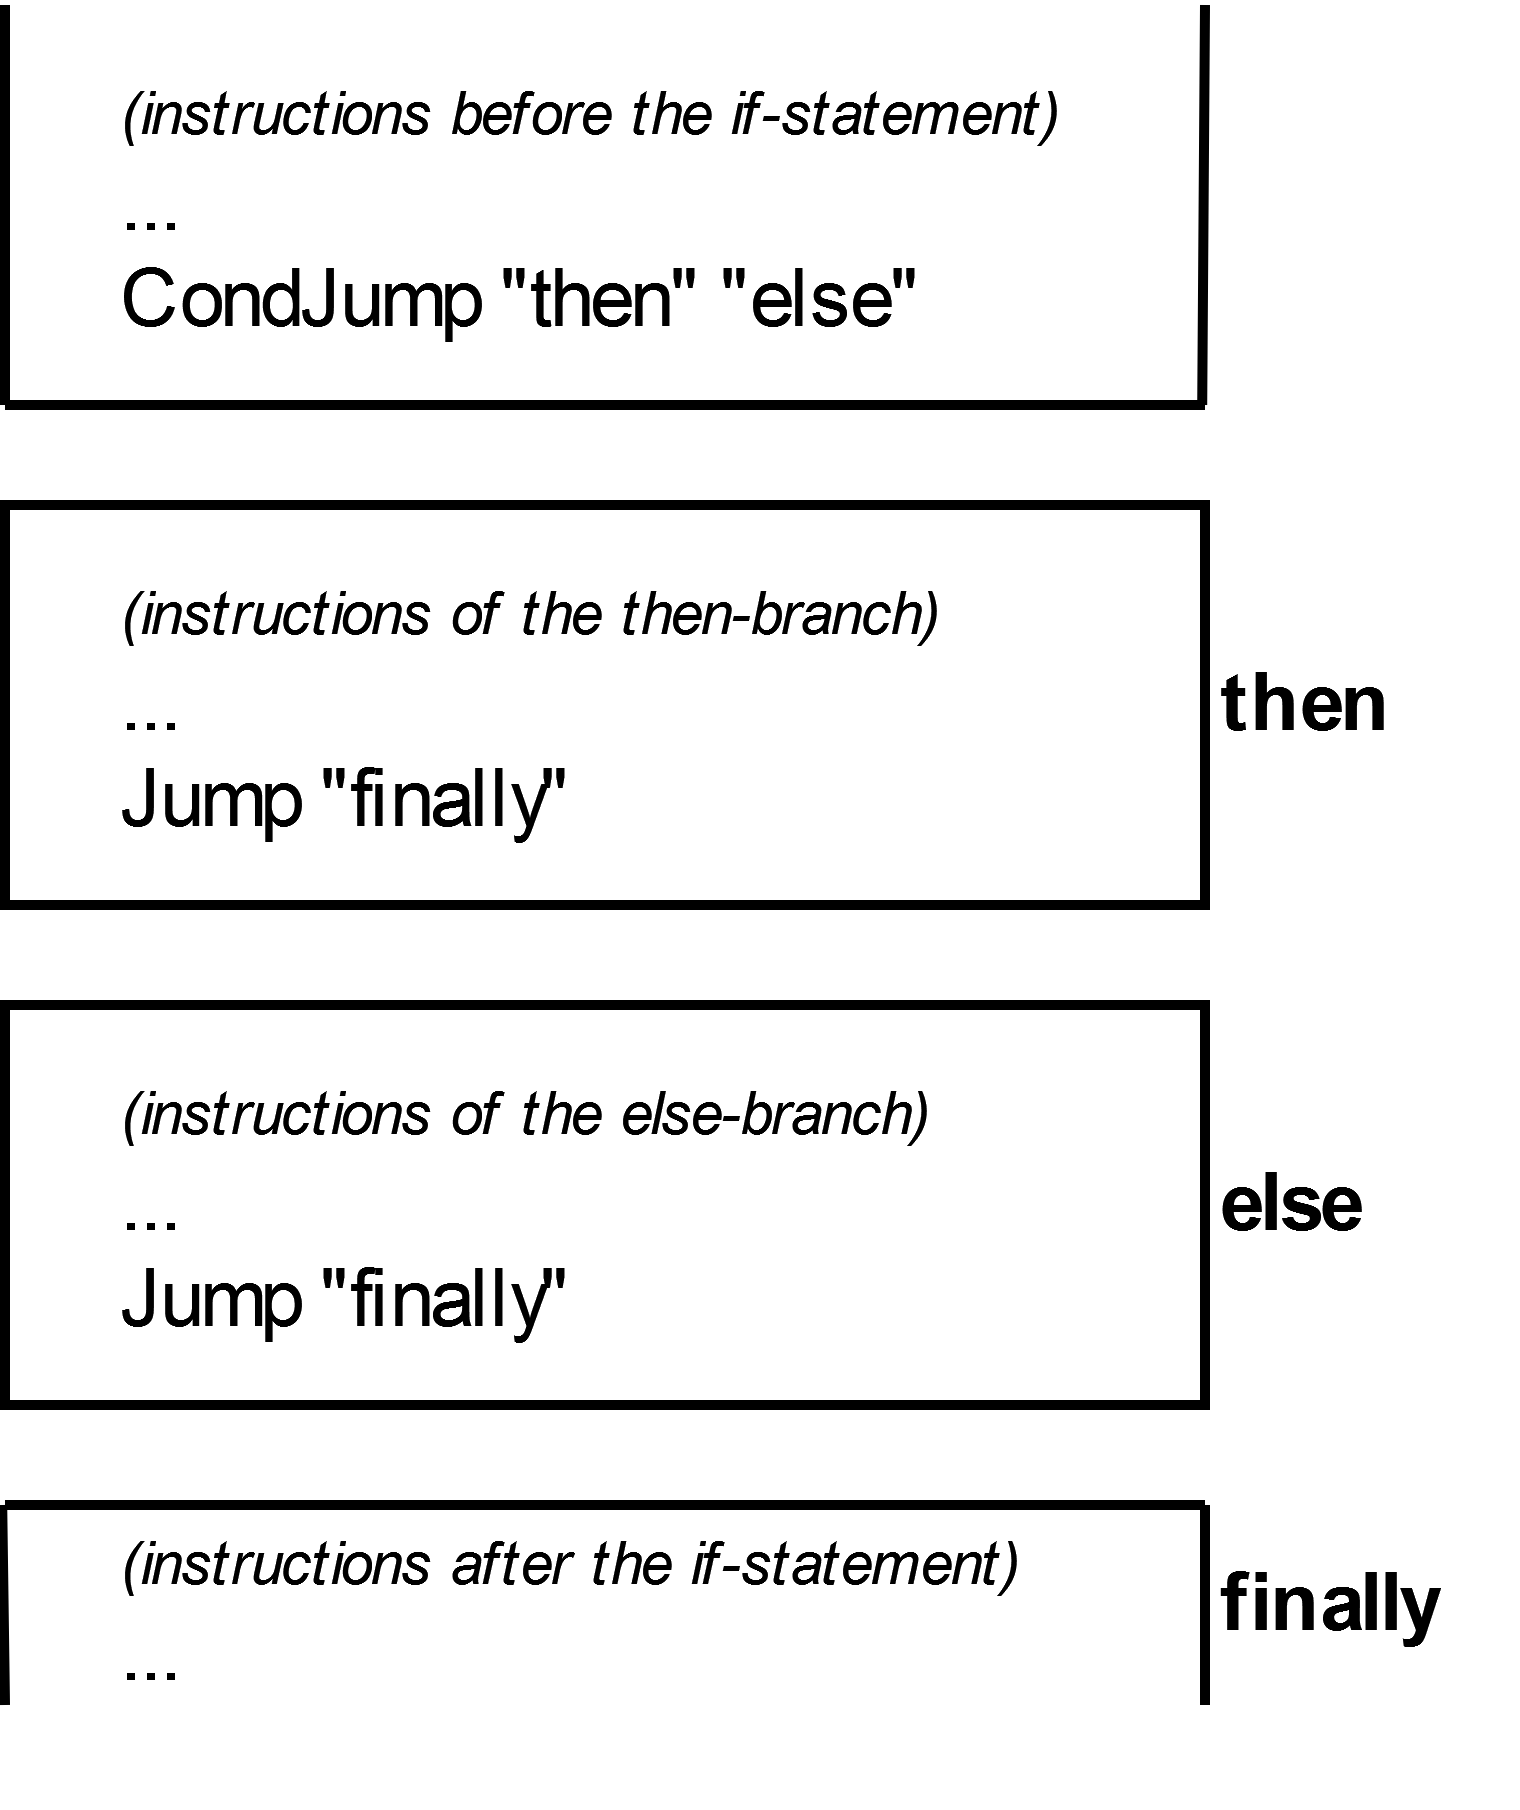
\includegraphics[width=5cm]{img/x86ir_if.png}}
	\hspace{1em}
	\subfloat[A while-statement in x86IR.\label{fig:x86ir_while}]{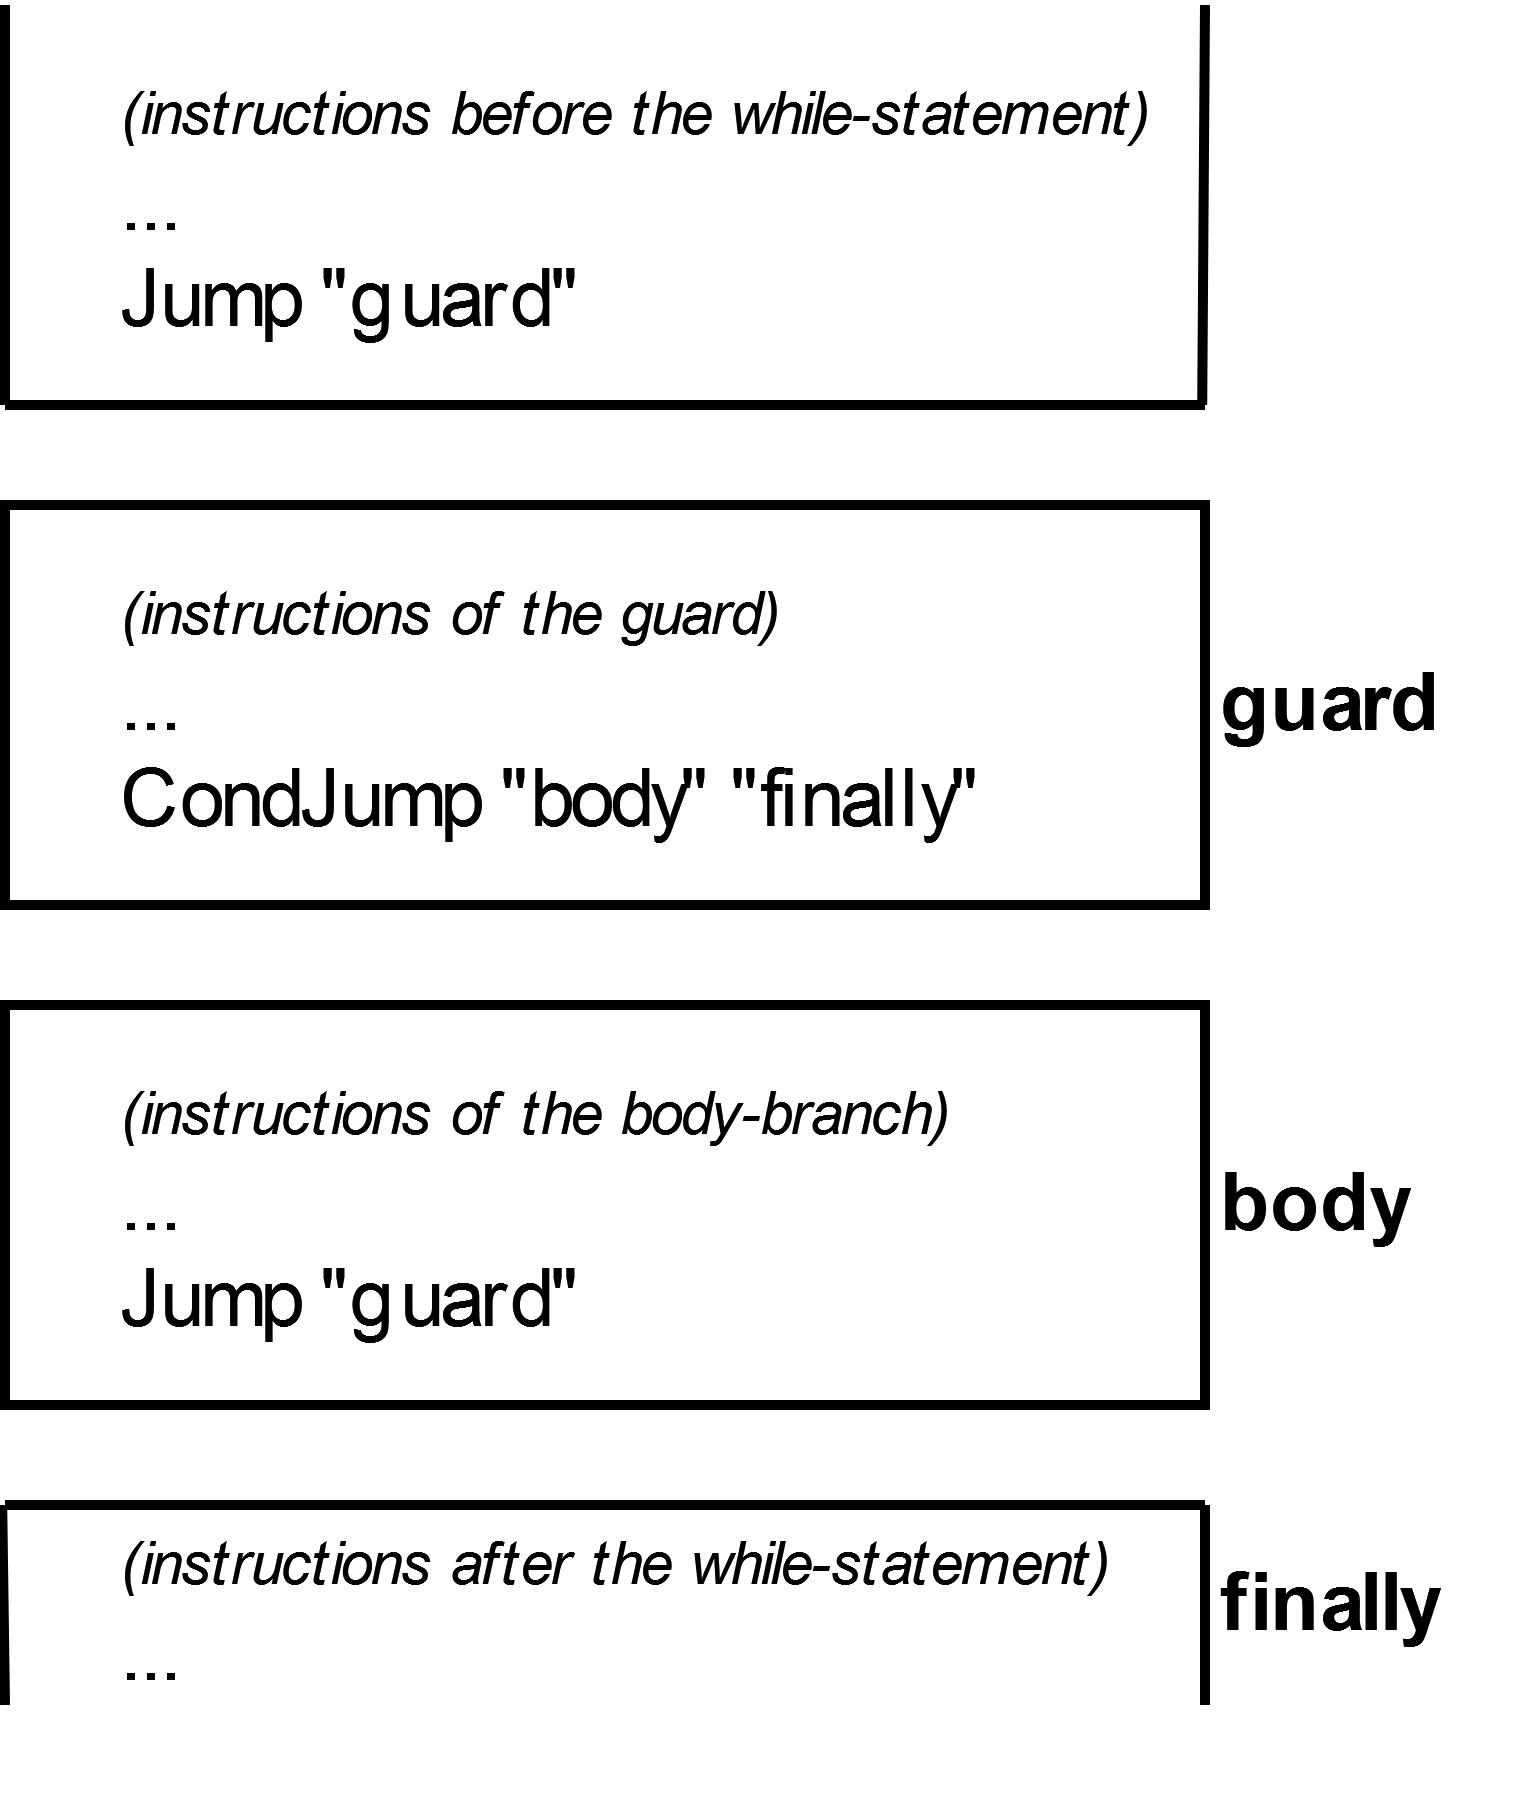
\includegraphics[width=5cm]{img/x86ir_while.png}}
	\caption{A branching in x86IR represented by basic blocks.}
	\label{fig:x86ir_branching}
\end{figure}

\subsection{Stack frame and calling conventions}\label{ssec:stack_frame}
As mentioned in \autoref{ssec:storage_org}, allocation and deallocation of a stack frame is a responsibility of the compiler. Before we move onto the generation of x86 assembly code, we will have to design how the allocation and deallocation will work in our compiler. For the design, we will be using a model situation, where function \emph{main} calls function \emph{foo}. The state of the stack before the call is shown in \autoref{fig:stack_precall}.

When \emph{foo} is being called, \emph{main} has to somehow pass function call arguments to \emph{foo}. Some calling conventions may use registers to pass the arguments \cite[Chap. 7]{calling_convention}, however we will be using stack. By doing so, we will implicitly have dedicated space for arguments on stack in case they will have to be spilled\footnote{\emph{Spilling} occurs when the register allocator cannot assign some virtual register to a physical one \cite[Chap. 7.2.3]{eng_comp} (e.g., when all of physical registers are occupied)---value of one of the physical registers gets spilled to stack, thus freeing up the physical register.} from a register during the register allocation. Therefore, \emph{main} has to push all arguments of the call onto the stack. After that, \emph{main} pushes an \emph{instruction pointer}\footnote{\emph{Instruction pointer} is a pointer that points to the next instruction that will be executed.} (IP) onto the stack. It will be used to decide which instruction to execute next after \emph{foo} returns from its call. Finally, \emph{foo} is called and the control flow is transferred to it.

Function \emph{foo} is now in control of the flow and before it executes any of its basic blocks, it has to persist BP of \emph{main} by pushing it onto the stack. Then, \emph{foo} has to set BP to point to the start of the \emph{foo}'s stack frame---this is done by copying SP into BP. Finally, \emph{foo} allocates enough space on the stack for local variables and temporary values of \emph{foo} (this is done by moving the SP downwards) and starts executing its basic blocks. The state of the stack after these actions is shown in \autoref{fig:stack_call}.

When \emph{foo} reaches a return statement, it has to somehow pass the return value to the stack frame of \emph{main}. Our convention will be to use the register RAX. After the return value is stored, SP is copied into BP and previously saved BP of \emph{main}'s stack frame is loaded back from the stack. Finally, \emph{foo} transfers control flow back to \emph{main} using the IP that was stored by \emph{main} on the stack. At this point, the stack frame of \emph{foo} has been completely deallocated.

Before \emph{main} executes its next instruction, previously pushed arguments of the call are removed from the stack by moving SP upwards. After that, \emph{main} continues to execute its instructions. The state of the stack is now the same as it was before the call (see \autoref{fig:stack_precall}).

\begin{figure}
	\centering
	\subfloat[Before the call of \emph{foo}.\label{fig:stack_precall}]{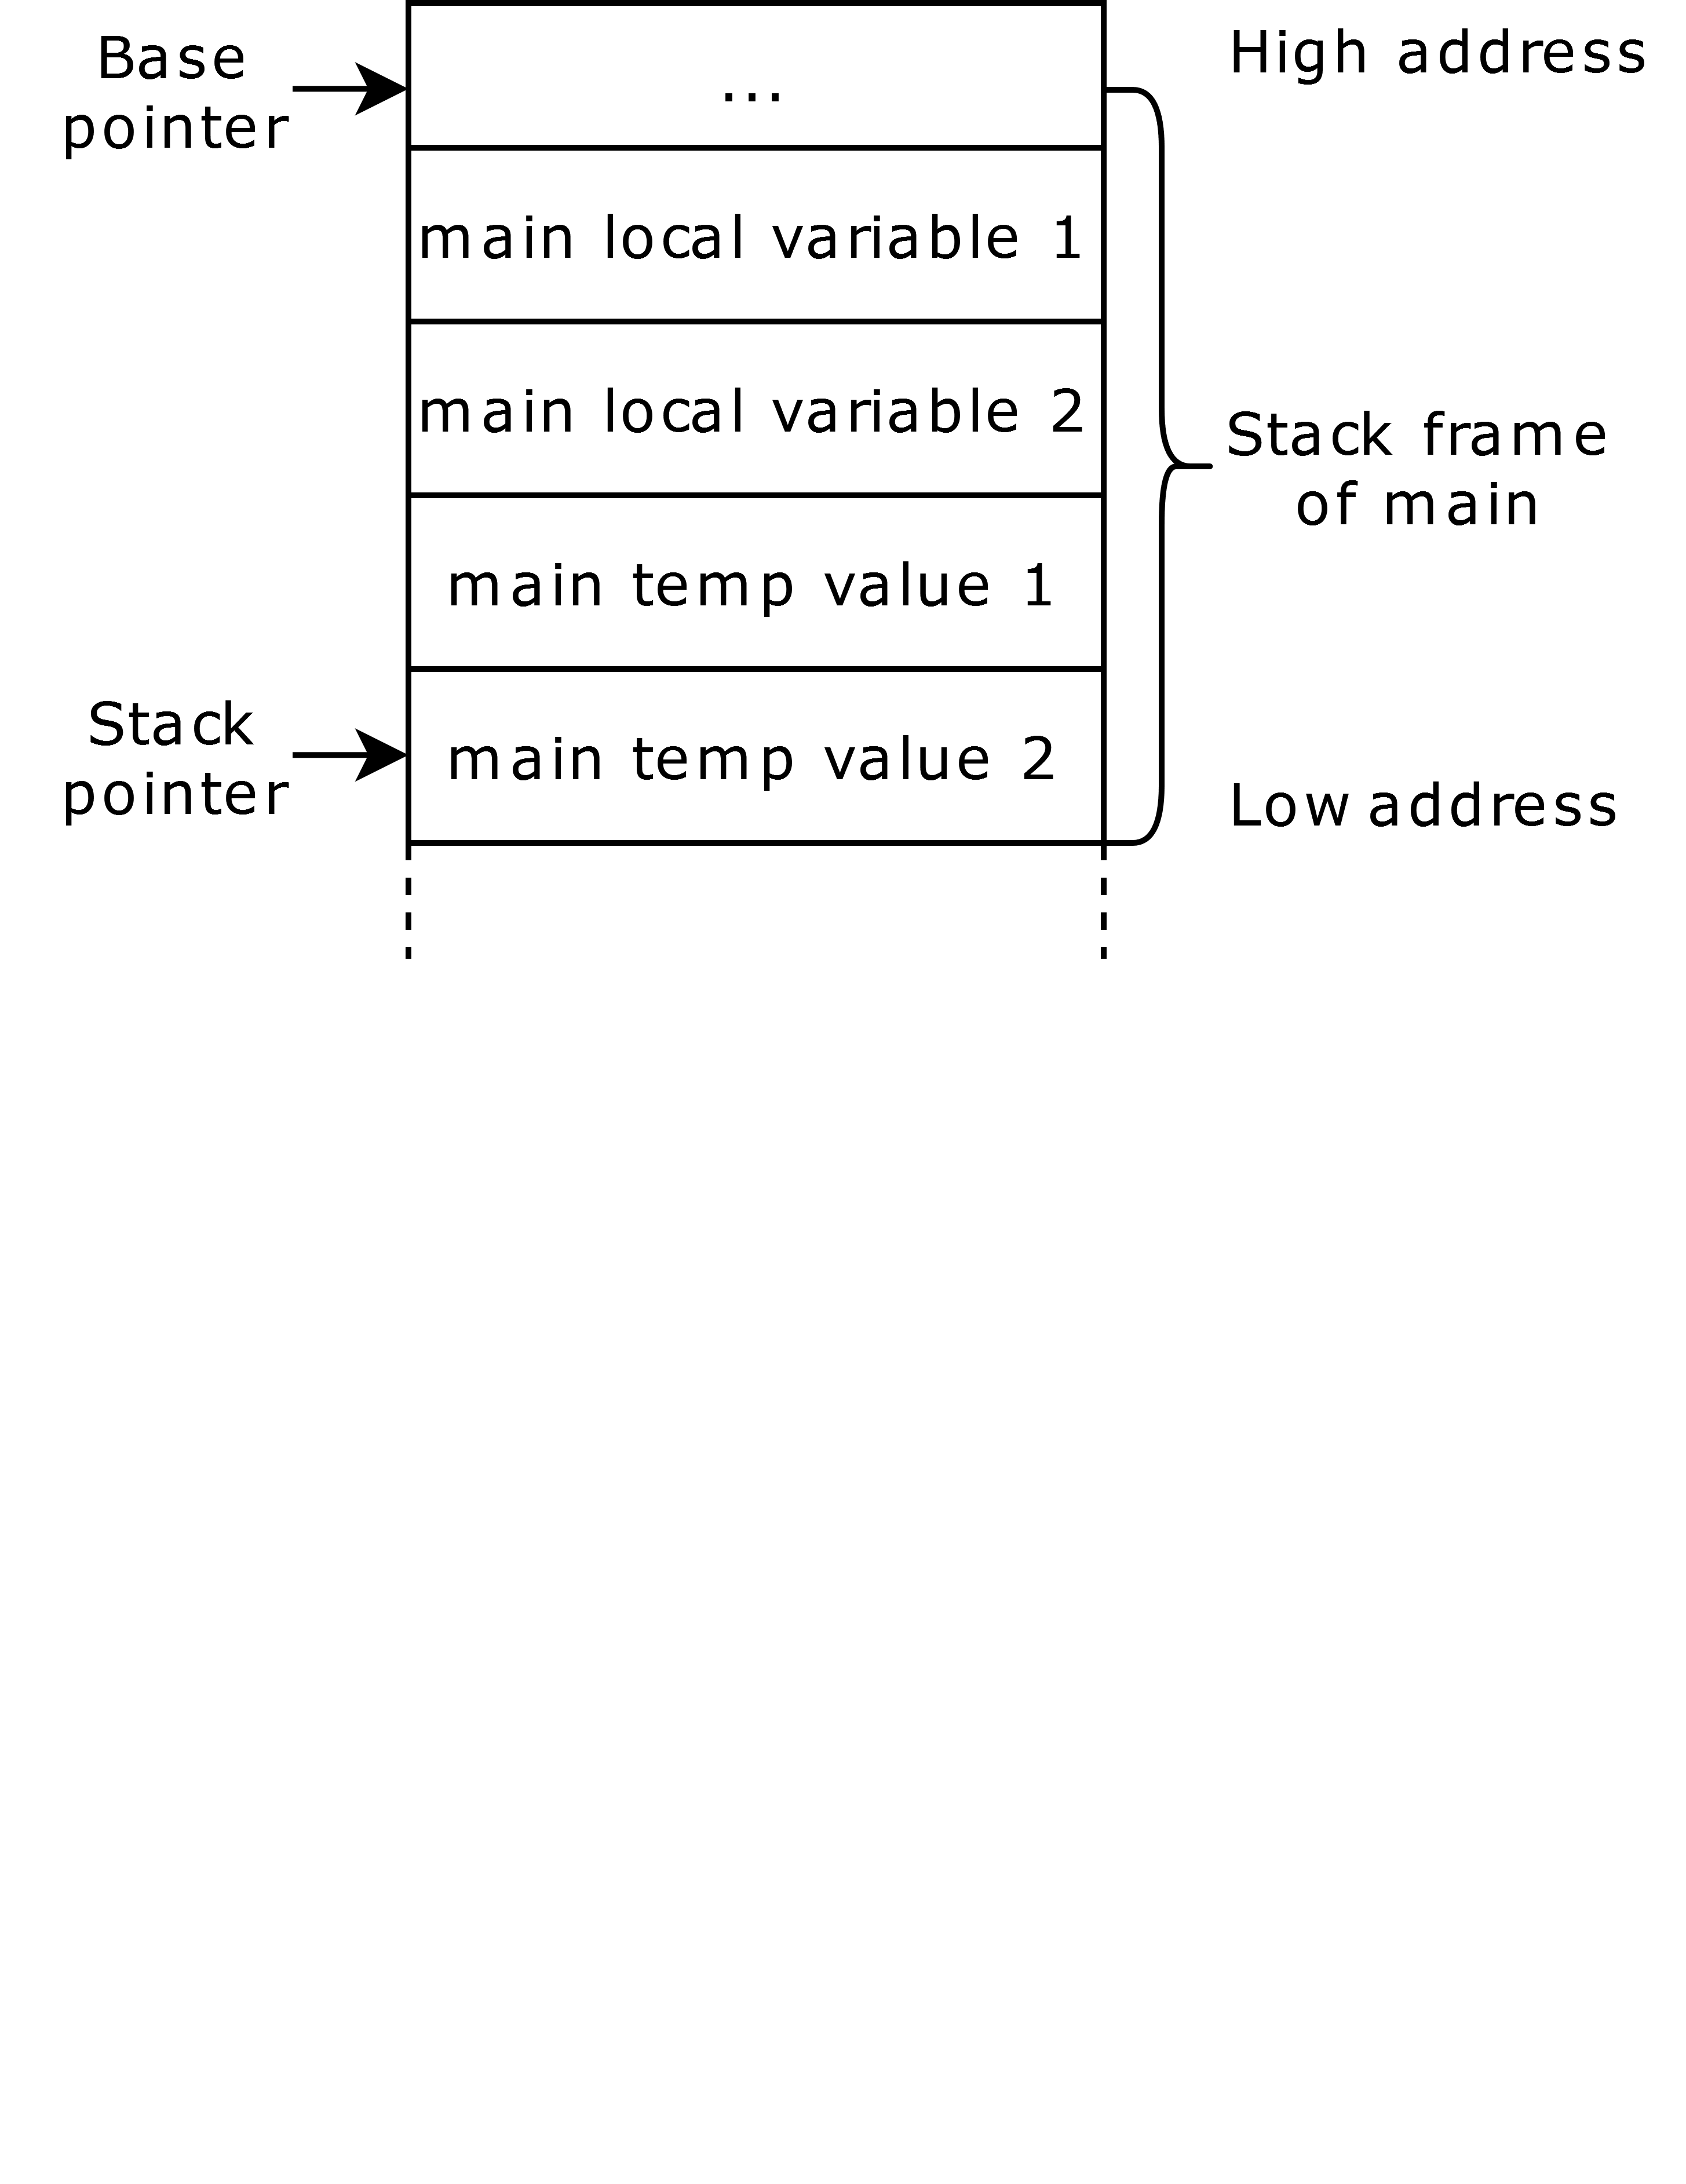
\includegraphics[width=6cm]{img/stack_precall.png}}
	\hspace{1em}
	\subfloat[After the call of \emph{foo}.\label{fig:stack_call}]{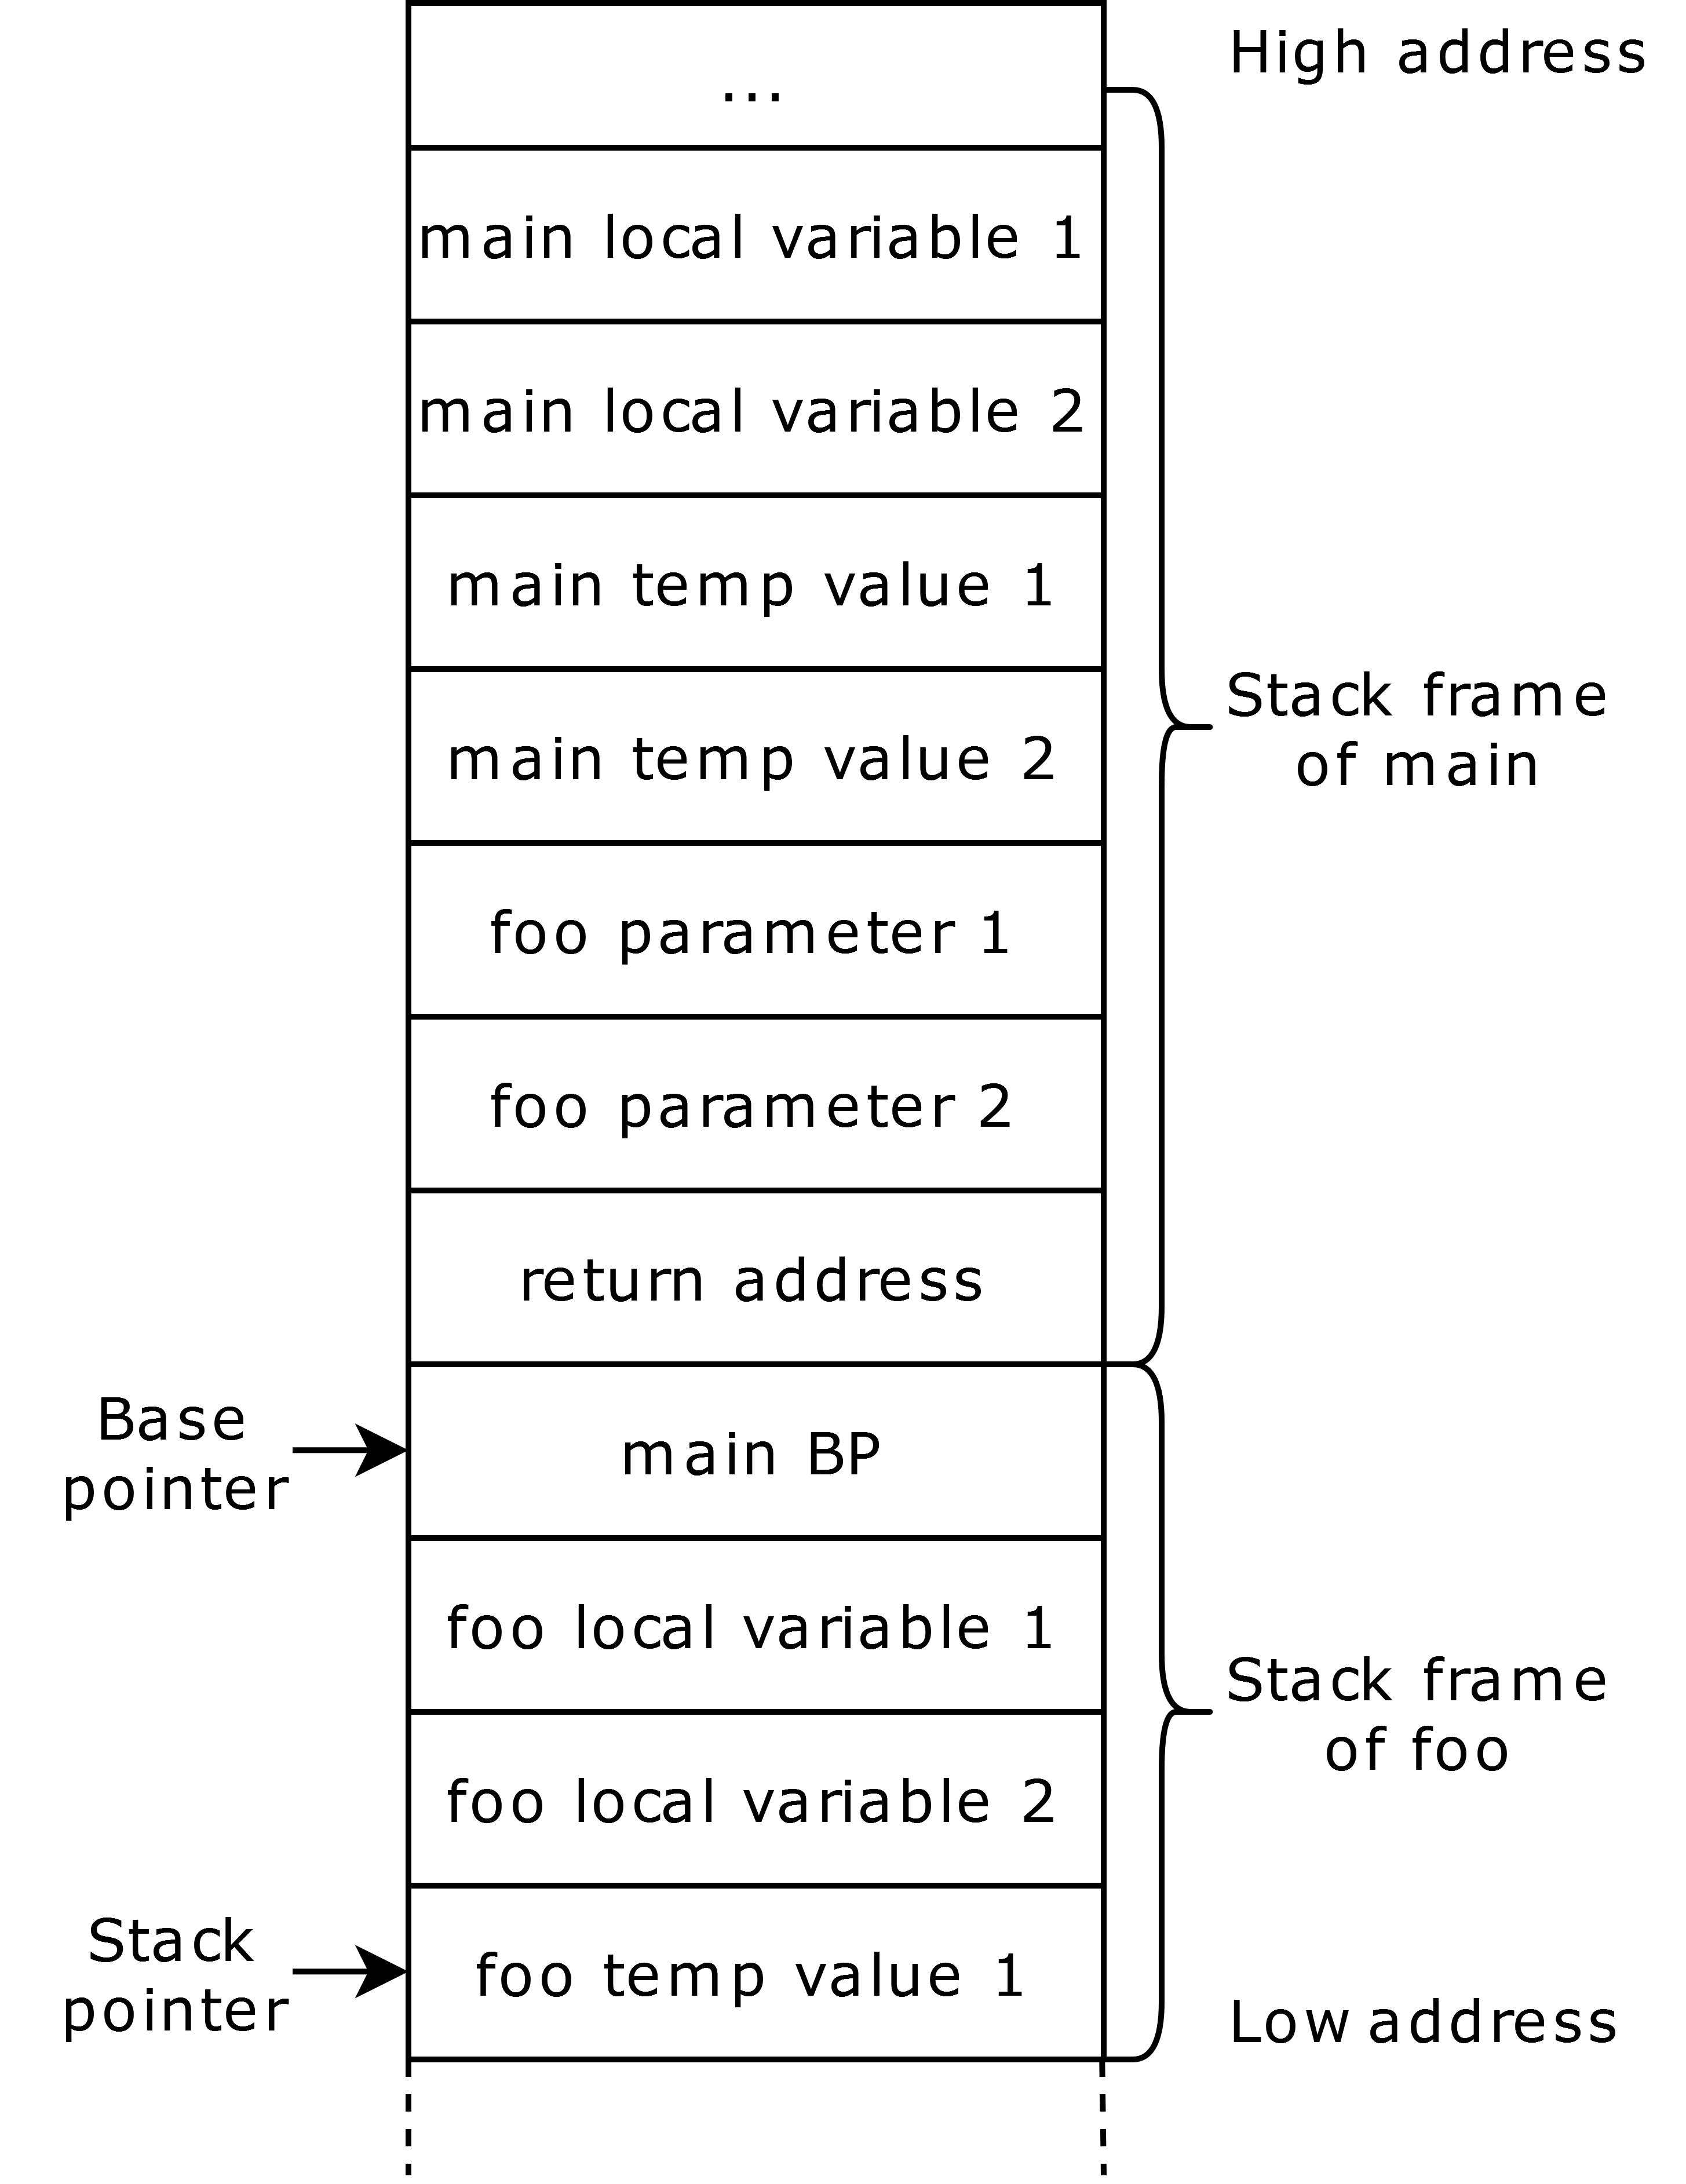
\includegraphics[width=6cm]{img/stack_call.png}}
	\caption{Comparison of stack states before and after calling \emph{foo}.}
	\label{fig:stack_state}
\end{figure}

\subsection{Code generation of x86 assembly}\label{ssec:x86_code_gen}
With better understanding of allocation and deallocation of a stack frame, we can move on to the second component of the backend---\emph{x86IR Compiler}. Its goal will be to transform x86IR into x86 assembly. 

Before we start compiling each function of the x86IR, we have to define the initial x86 program entry point with the label \texttt{\_start}\footnote{This particular label name is recognized by the standard system linkers \cite[Chap. 4.6]{x86_assembly}.}. Then we will have to assign an address to each function of the program (since functions can be referenced and dereferenced in microC). The microC program is then run using the \texttt{call} instruction, which will call the entry function of the microC program (usually the one called \emph{main}). After that, the program is terminated by calling \texttt{exit} (from \emph{libc}\footnote{\url{https://man7.org/linux/man-pages/man7/libc.7.html}}). The other option would be to use \texttt{sys\_exit} syscall, however since we will use other \emph{libc} functions like \texttt{printf} or \texttt{scanf}, we will keep things consistent and use \emph{libc} \texttt{exit}. We then continue by compiling each function of the program.

\paragraph*{Function} Entry point of a function will be a label with name of the function, which is followed by instructions that take care of updating BP and allocating enough space on the stack for local variables and temporary values (recall \autoref{ssec:stack_frame} where we discussed what happens, when a function is given control of the flow). After that, we will compile each \emph{basic block} of the function.

\paragraph*{Basic block} Similarly to a function, the entry point of a \emph{basic block} will be a label with its name. Then we will compile each instruction of the \emph{basic block} (their compilation will be discussed in the following paragraphs). After each compiled x86IR instruction we will have to make sure that registers only contain live values---since we only have a finite number of registers, we do not want to keep having registers cluttered with dead values (e.g., operands of an instruction that has been already executed). To decide which values are dead, we will be using a \emph{live instruction analysis}, which will be covered in the following subsection.

\paragraph*{Alloc} The \emph{Alloc} instruction allocates memory on the stack for a local variable. The size of the allocated memory depends on the type of the instruction. Since local variables are addressed using a negative offset from BP (recall \autoref{fig:stack_state}), we will assign a new offset to this variable. The negative offset from BP will be the address of the variable.

\paragraph*{ArgAddr} The \emph{ArgAddr} instruction is very similar to \texttt{Alloc}, the only difference is that the memory is allocated for the function's argument and the assigned offset is positive. The positive offset from BP will be the address of the function's argument.

\paragraph*{HeapAlloc} The \emph{HeapAlloc} instruction allocates memory on the heap. To do this, we will have to call the function \texttt{malloc} (from \emph{libc}), which takes care of the allocation and returns the address of the allocated memory. The call consists of these steps:
\begin{enumerate}
    \item Save caller saved registers by pushing them onto the stack---these registers are not preserved across a function call. The caller saved registers are: \texttt{rax} (since it will contain the return value), \texttt{rcx}, \texttt{rdx}, \texttt{rsi}, \texttt{rdi}, \texttt{r8}, \texttt{r9}, \texttt{r10}, and \texttt{r11} \cite[Chap. 12.8.3]{x86_assembly}.
    \item Align stack to 16 bytes---before every call, the stack has to be aligned to 16 bytes \cite[Chap 6.2.2]{intel_x86}.
    \item Load the first argument of \texttt{malloc} (size of the allocated memory)---following the Linux calling convention, the first argument of a function is stored in the register \texttt{rdi} \cite[12.8.1]{x86_assembly}.
    \item Finally, call the function.
\end{enumerate}
After the call, the address of the memory will be stored in \texttt{rax}. Now we will dealign stack and restore caller saved registers. Lastly, we will initialize the address with the value specified by the \emph{HeapAlloc} instruction.

\paragraph*{Store} The \emph{Store} instruction represents a write to memory, and its arguments are the value to store and the address at which to store it. If the value is a composed type (e.g., a record), the value is actually an address of the composed value we will be storing (its contents are typically stored on stack or heap). We will use this address to access each part of the composed value and move it to the destination address. Any other type is simply moved from a register to the destination address.

\paragraph*{LoadImm} The \emph{LoadImm} instruction loads an immediate value (signed integer). We will do this by simply moving the value into a register. Since microC uses 32-bit integers, we will use only the lowest 32-bits of the 64-bit register\footnote{This is done by, e.g., accessing the register \texttt{rax} as \texttt{eax} \cite[Chap. 2.3.1.1]{x86_assembly}.}. 

\paragraph*{LoadComposed} The \emph{LoadComposed} instruction loads a composed value (e.g., a record). Since composed types consist of multiple values, we cannot move them into a register as we did with an immediate value. Instead, we will allocate space on the stack and move each part of the composed type there. Then we will move the address of its first member into a register---this address will represent the “value” of the composed type.

\paragraph*{Load} The \emph{Load} instruction loads a value from a memory address. We will do this by accessing the address and moving its content into a register.

\paragraph*{GetAddr} The \emph{GetAddr} instruction returns the address of a variable. Since the address of a variable is offset from BP, which was assigned to the variable by instruction \emph{Alloc} or \emph{ArgAddr}, we will simply find the assigned offset and load the address into a register.

\paragraph*{GetAddrOffset} The \emph{GetAddrOffset} instruction returns the address of a sub\-element of a composed type. Arguments of this instruction are an address of the composed type and an offset, therefore we will simply add the offset to the address and load the result of this addition into a register.

\paragraph*{BinOp} The \emph{BinOp} instruction performs a binary operation and returns its result. The most simple are the operations \emph{addition}, \emph{subtraction}, and \emph{multiplication}, which we will perform by emitting x86 instructions \texttt{add}, \texttt{sub}, and \texttt{imul}, respectively.

\emph{Division} is a little more complicated, since the first operand (dividend) of the x86 instruction \texttt{idiv} spans over two registers---\texttt{rdx} (high bits)  and \texttt{rax} (low bits) \cite[Page 3-487]{intel_x86}. We will move dividend into \texttt{rax} and set register \texttt{rdx} to 0. After executing \texttt{idiv}, the result of the operation will be stored in the register \texttt{rax}.

In case of \emph{equal} and \emph{greater-than}, we will compare their operands. If the comparison is true, we will load a value $1$ into a register. Otherwise, we will load value $0$.

\paragraph*{LoadInput} The \emph{LoadInput} instruction loads an integer from a standard input. Similarly to \emph{HeapAlloc}, we will have to use extern function \texttt{scanf} (from \emph{libc}), which scans the input using the provided format string. The call of the function consists of these steps:
\begin{enumerate}
    \item Save caller saved registers by pushing them onto the stack.
    \item Align stack to 16 bytes.
    \item Load the first argument of \texttt{scanf} into the register \texttt{rdi}---format string, which defines layout of the scanned input. Since we are loading a 32-bit signed integer, we will use the format string \texttt{\%ld} (long integer).
    \item Load the second argument into the register \texttt{rsi}\footnote{The register \texttt{rsi} is used for the second argument of a function in the Linux calling convention \cite[12.8.1]{x86_assembly}.}---address of the memory, where the scanned integer will be stored.
    \item Finally, call the function.
\end{enumerate}
Right after the call, we will dealign stack. If the return value of the call\footnote{The function \texttt{scanf} returns the number of successfully matched input items \cite{scanf}.} (stored in \texttt{rax}) is $1$, we will then move the loaded integer from the address which we provided to \texttt{scanf} into a register. Otherwise, EOF was reached and we will load $-1$ instead. Lastly, we will restore caller saved registers.

\paragraph*{Print} The \emph{Print} instruction writes an integer to a standard output. Once again, we will have to rely on extern function \texttt{printf} (from \emph{libc}), which writes an output using the provided format string. The call of the function consists of these steps:
\begin{enumerate}
    \item Save caller saved registers by pushing them onto the stack.
    \item Align stack to 16 bytes.
    \item Load the first argument of \texttt{printf} into a register \texttt{rdi}---format string, which defines layout of the printed output. We will use the same format string as we did for \emph{LoadInput}---\texttt{\%ld} (long integer).
    \item Load the second argument into a register \texttt{rsi}---the value to be printed.
    \item Finally, call the function.
\end{enumerate}
After the call, we will just dealign stack and restore caller saved registers.

\paragraph*{Call} The \emph{Call} instruction transfers the control flow to the called function. The call consists of these steps:
\begin{enumerate}
    \item Save current state of registers by pushing them onto the stack.
    \item Align stack to 16 bytes.
    \item Load the function that will be called.
    \item Load all arguments of the function call---our calling convention is to pass function call arguments using the stack, therefore we will push them in order onto the stack.
    \item Call the function using x86 instruction \texttt{call}.
    \item Clear arguments from the stack.
    \item Dealign the stack.
    \item Restore previous state of registers from the stack.
\end{enumerate}
After these steps, the return value will be stored in the register \texttt{rax}. In case the return value is a composed type, the value stored in the register \texttt{rax} is just its address pointing to a deallocated frame stack of the called function. Therefore, we will have to use this address to move each part of the composed type into the current stack frame.

\paragraph*{Return} The \emph{Return} instruction stores the return value and returns the control flow to the caller of the current function. Since our calling convention is to use register \texttt{rax} as the register for return values, we will move the return value into it. Then we will reset SP by overwriting it with BP and restore BP of the caller function by loading it from the stack. Lastly, we will emit x86 instruction \texttt{ret}.

\paragraph*{CondJump} The \emph{CondJump} instruction transfers the control flow to a different basic block based on the value of the condition. We will compare the value of the condition with $0$ and then emit x86 instruction \texttt{je}, which will jump to “false-branch” basic block if the compared values are equal. Then we will emit \texttt{jmp} which will jump to “true-branch” basic block.

\paragraph*{Jump} The \emph{Jump} instruction transfers the control flow to a different basic block. We will do this by simply emitting x86 instruction \texttt{jmp}.

\subsection{Live instruction analysis}\label{ssec:lia}
As mentioned earlier, the x86 target machine has only a finite number of registers. Keeping dead values in them will result in a faster congestion of registers, which leads to more spilling (and therefore less efficient code). To decide which values are no longer required to keep in registers, we will be using a live instruction analysis.

The scope of the analysis will be a single basic block $B$, which can be viewed as a sequence of $n$ instructions $I_0, I_1, ..., I_n$. The result of the analysis will be sets of instructions (for each instruction $I_i \in B$), whose result is live \emph{after} the execution of the instruction $I_i$, which we will denote as $LIVE(I_i)$. The result of the analysis can be defined by the following recurrence relation, where $op(I_i)$ denotes operands of an instruction $I_i$:

\begin{align}
    LIVE(I_n) &= \emptyset\\
    LIVE(I_{i-1}) &= \Big(LIVE(I_i) \cup op(I_i)\Big) \setminus \{I_i\}
\end{align}

No value is live after the last instruction of basic block (relation 2.1). Only values that are yet to be used as operands of some instruction (that has not been executed yet) are live (relation 2.2).

\subsection{Peephole optimizations}
The last component of the backend will be \emph{Peepholer}. Its goal will be to take assembly produced by \emph{x86IR Compiler}, perform peephole optimizations, and produce optimized assembly.

The basic premise of peephole optimization is to examine short sequences of adjacent operations and find local improvements. This is done by having a sliding window which at each step observes a small number of operations, looking for a specific pattern that can be improved \cite[Chap. 11.5.1]{eng_comp}. See \autoref{fig:peephole} for an example of a sliding window that has the size of two instructions---the first observed instruction copies the content of \texttt{rbx} to \texttt{rax}. The following instruction then copies the content of \texttt{rax} back to \texttt{rbx}, which is in this case a redundant operation that can be safely eliminated.

\begin{figure}
    \centering
    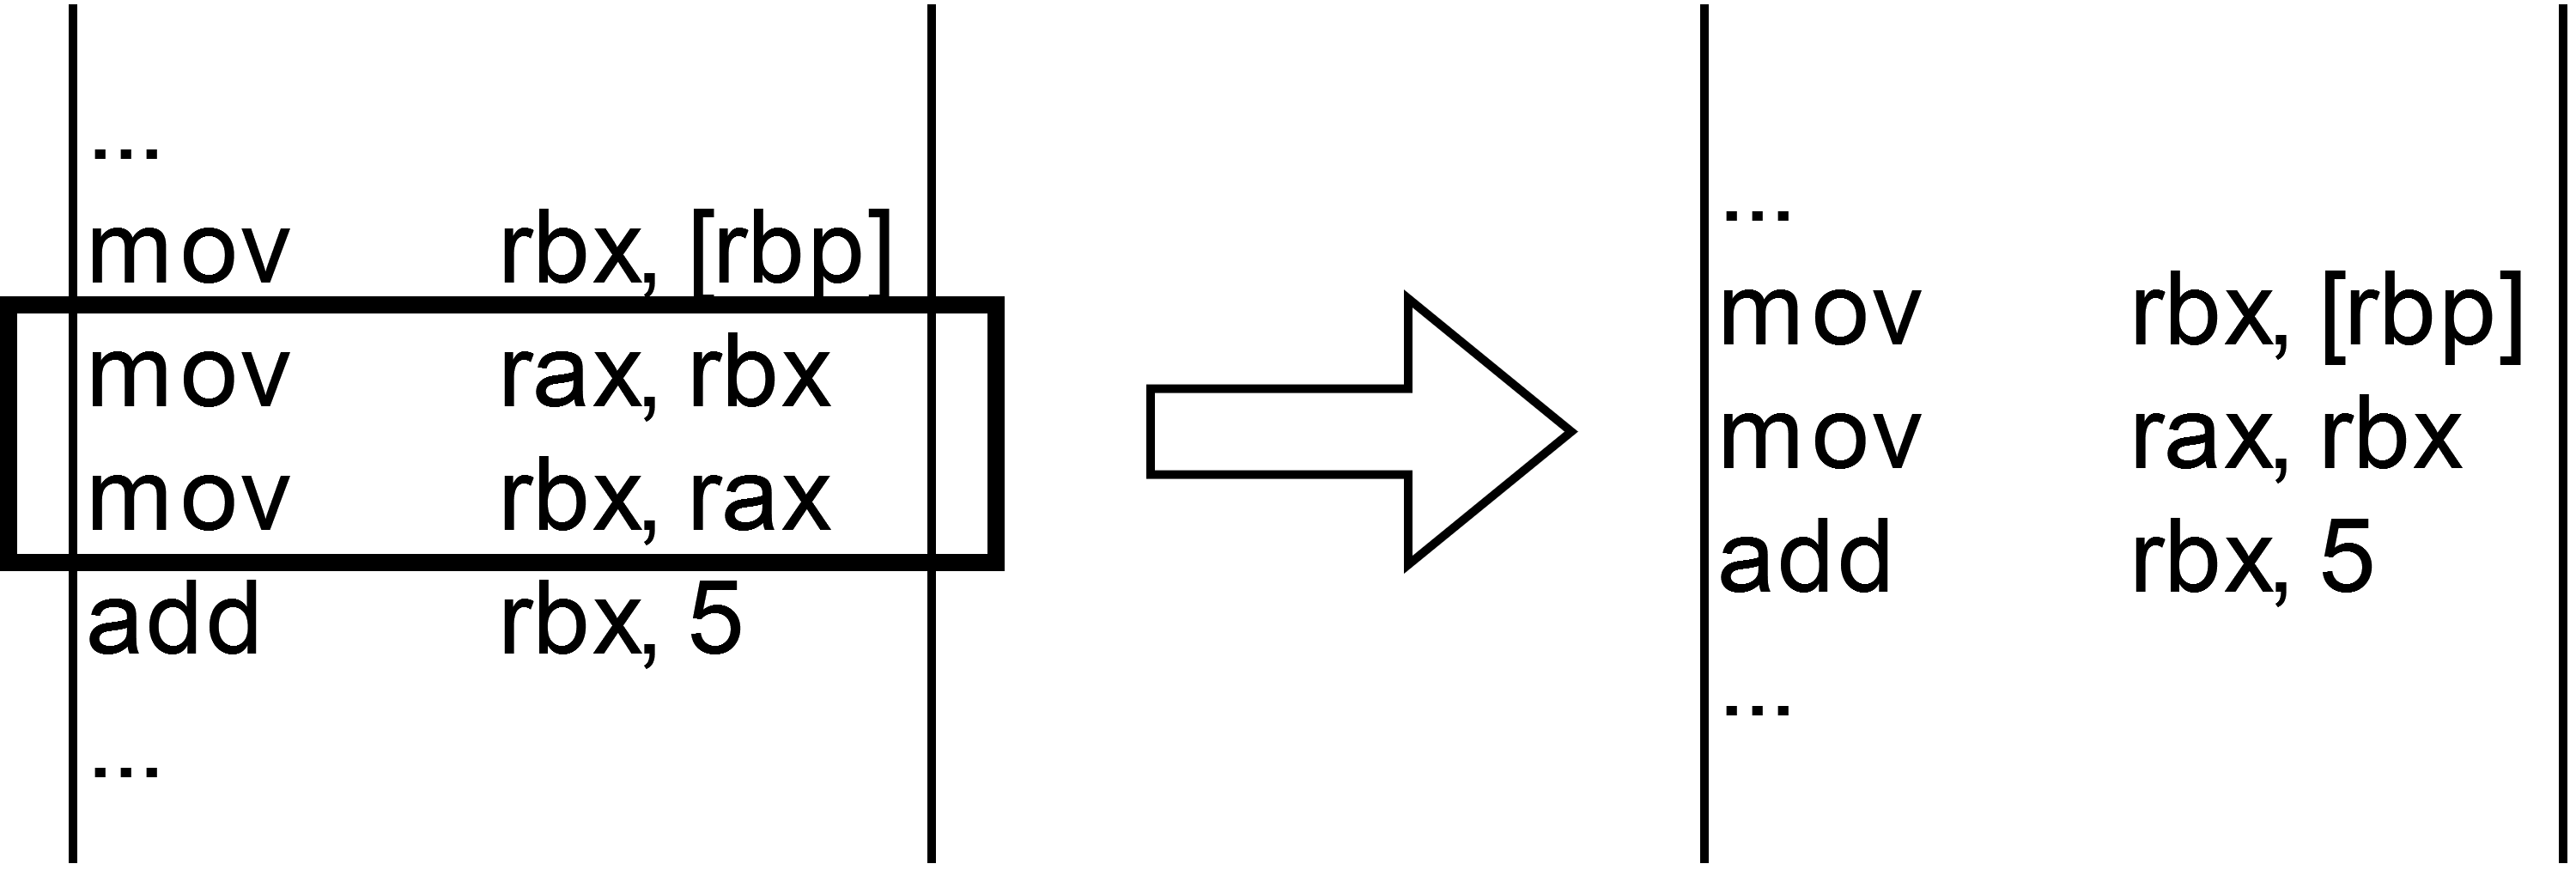
\includegraphics[width=9cm]{img/peephole.png}
    \caption{A peephole optimization.}\label{fig:peephole}
\end{figure}

Our peepholer uses sliding window that has size of one and two instructions. The 1-instruction improvements mostly consist of deletion of useless operations, usage of algebraic laws, or usage of instructions designed for special operand cases. The 2-instruction improvements consist of combining of several algebraic operations into one equivalent and eliminating redundant move operations. The overview of all rewrite-rules we will be using is shown in \autoref{tab:peephole_rules}.

\begin{table}
\footnotesize
\begin{minipage}{.45\linewidth}
    \centering
    \begin{tabular}{|l|l|}
        \hline
        \multicolumn{2}{|c|}{2-instruction sliding window} \\
        \hline
        Pattern & Replace with\\
        \hline
        \hline
        \makecell{ \texttt{jmp l1} \\ \texttt{l1:} } & \texttt{l1:}\\
        \hline
        \makecell{ \texttt{add o1, i1} \\ \texttt{add o1, i2} } & \texttt{add o1, }$ev(i1 + i2)$\\
        \hline
        \makecell{ \texttt{add o1, i1} \\ \texttt{sub o1, i2} } & \texttt{add o1, }$ev(i1 - i2)$\\
        \hline
        \makecell{ \texttt{sub o1, i1} \\ \texttt{sub o1, i2} } & \texttt{sub o1, }$ev(i1 + i2)$\\
        \hline
        \makecell{ \texttt{sub o1, i1} \\ \texttt{add o1, i2} } & \texttt{sub o1, }$ev(i1 - i2)$\\
        \hline
        \makecell{ \texttt{imul o1, i1} \\ \texttt{imul o1, i2} } & \texttt{imul o1, }$ev(i1 \cdot i2)$\\
        \hline
        \makecell{ \texttt{shl o1, i1} \\ \texttt{shl o1, i2} } & \texttt{shl o1, }$ev(i1 + i2)$\\
        \hline
        \makecell{ \texttt{shr o1, i1} \\ \texttt{shr o1, i2} } & \texttt{shr o1, }$ev(i1 + i2)$\\
        \hline
        \makecell{ \texttt{mov o1, o2} \\ \texttt{mov o2, o1} } & \texttt{mov o1, o2}\\
        \hline
        \makecell{ \texttt{mov m1, r1} \\ \texttt{mov r2, m1} } & \makecell{ \texttt{mov m1, r1} \\ \texttt{mov r2, r1} }\\
        \hline
    \end{tabular}
\end{minipage}%
\begin{minipage}{.55\linewidth}
    \begin{tabular}{|l|l|}
        \hline
        \multicolumn{2}{|c|}{1-instruction sliding window} \\
        \hline
        Pattern & Replace with\\
        \hline
        \hline
        \texttt{add o1, 0} &\\
        \hline
        \texttt{add o1, 1} & \texttt{inc o1}\\
        \hline
        \texttt{add o1, -1} & \texttt{dec o1}\\
        \hline
        \texttt{add o1, o1} & \texttt{shl o1, 1}\\
        \hline
        \texttt{sub o1, 0} &\\
        \hline
        \texttt{sub o1, 1} & \texttt{dec o1}\\
        \hline
        \texttt{sub o1, -1} & \texttt{inc o1}\\
        \hline
        \texttt{sub o1, o1} & \texttt{mov o1, 0}\\
        \hline
        \texttt{imul o1, 0} & \texttt{mov o1, 0}\\
        \hline
        \texttt{imul o1, 1} &\\
        \hline
        \makecell{ \texttt{imul o1, i1} \\ if \texttt{i1} is power of 2 } & \texttt{shl o1, }$ev(log_2(i1))$\\
        \hline
        \texttt{shl o1, 0} &\\
        \hline
        \texttt{shr o1, 0} &\\
        \hline
        \texttt{mov o1, o1} &\\
        \hline
        \texttt{mov o1, 0} & \texttt{xor o1, o1}\\
        \hline
        \texttt{mov [o1+0], o2} & \texttt{mov [o1], o2}\\
        \hline
        \texttt{mov o1, [o2+0]} & \texttt{mov o1, [o2]}\\
        \hline
    \end{tabular}
\end{minipage}%
\\
\begin{tabular}{ll}
    \multicolumn{2}{l}{\emph{Notes:}}\\
    \texttt{l}---label & \texttt{r}---register\\
    \texttt{o}---instruction operand & \texttt{m}---memory access\\
    \texttt{i}---constant integer & $ev$---evaluation of a binary operation\\
\end{tabular}
\caption{The rewrite-rules for 2-instruction and 1-instruction sliding window.}\label{tab:peephole_rules}
\end{table}

\subsection{Summary of the backend}\label{ssec:backend_design_summary}
This concludes design of every component of the backend. By putting them all together (as illustrated in \autoref{fig:microc_backend}), we get a backend that takes a CFG from a middleend, transforms it into an x86 assembly, performs peephole optimizations on the assembly, and produces an optimized x86 assembly.

\begin{figure}
    \centering
    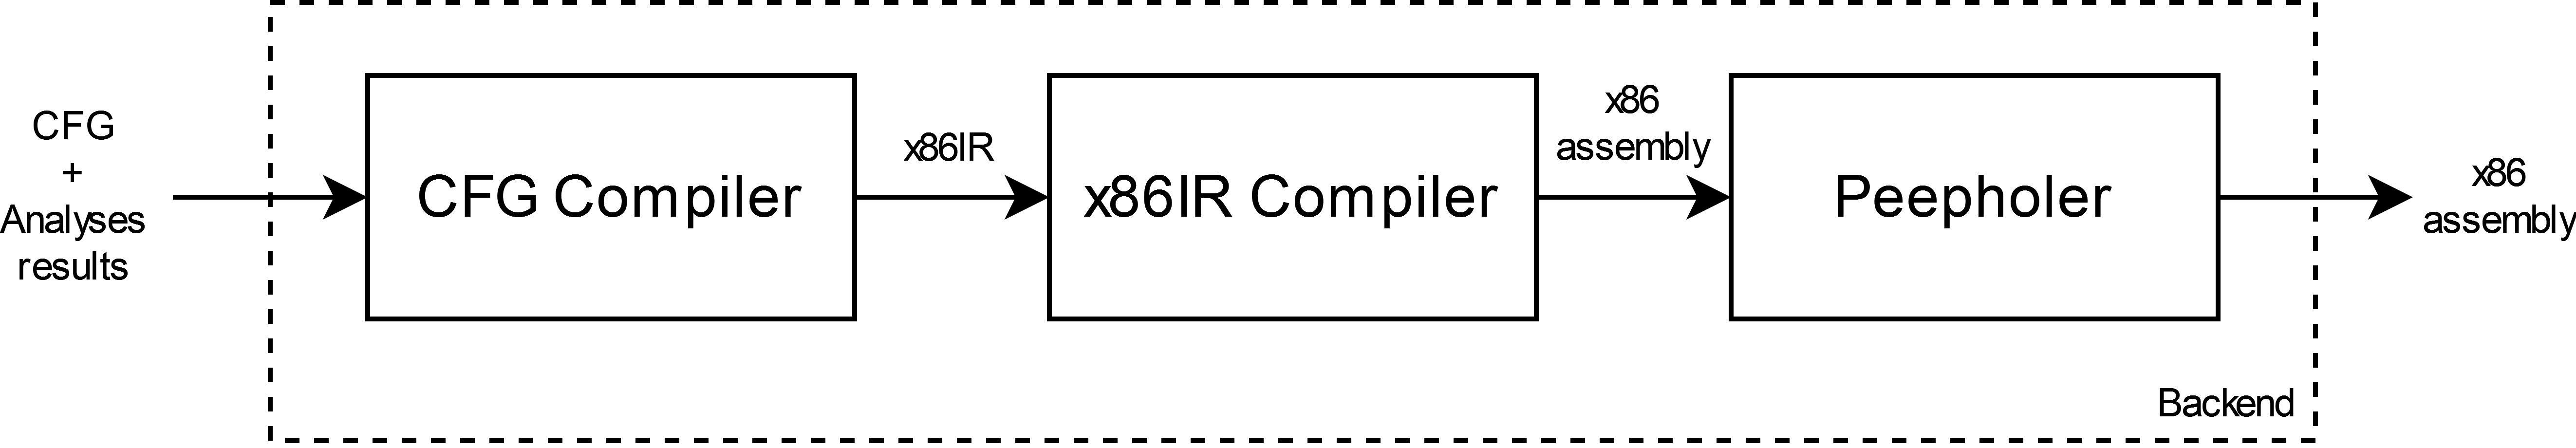
\includegraphics[height=2.2cm]{img/microc_backend.png}
    \caption{The backend of the microC compiler.}\label{fig:microc_backend}
\end{figure}

\chapter{Implementation}
With the design of the microC compiler out of the way, we can move on to its implementation. In the first part of this chapter we discuss the implementation of each part of the compiler (frontend, middleend, and backend), located in the folder \texttt{microc-compiler/src/main/scala/microc}. In the second part, we cover tests and documentation of the implementation.

As stated in the introduction of this thesis, the implementation of the compiler should be easy to read and follow, since it will be used as an educational material for students of the NI-APR course. General ways to achieve that are, e.g., proper commenting and documentation, consistent indentation, following DRY (Don't Repeat Yourself) principle, or using meaningful names for variables and functions. In addition to these principles, we will also take advantage of some useful Scala features; e.g., since Scala is not only an object-oriented programming language, but also a functional programming language \cite[Chap. 1.2]{scala}, we can avoid deep level of nesting (which are often harder to follow) by writing code in a more functional style. Take \autoref{lst:iter_for} and \autoref{lst:iter_fun} as an example, which are two ways of iterating over non-terminating instructions of an x86IR program---the first one is an imperative for-cycle approach and the second one is a functional approach. The latter one is much easier to follow, since it does not introduce multiple levels of nesting.

On the other hand, there are some Scala features that we will be avoiding for the sake of code clarity. The most notable example of such feature are \emph{implicit conversions}\footnote{\emph{Implicit conversions} allow the Scala compiler to convert one type to another by utilizing implicit classes or methods defined by the programmer \cite[21.1]{scala}.}, which are considered (even by the author of Scala, Martin Odersky \cite{impl_conv}) “evil”, since they make it hard to see what goes on in the code (e.g., side-effects or complex computations), because they are applied by the Scala compiler on the background.

\begin{listing}[H]
	\inputminted[tabsize=2,breaklines,bgcolor=codebg]{scala}{snippets/iter_for.m}
	\caption{For-cycle approach to iterating over non-terminating instructions of a program.}
	\label{lst:iter_for}
\end{listing}

\begin{listing}[H]
	\inputminted[tabsize=2,breaklines,bgcolor=codebg]{scala}{snippets/iter_fun.m}
	\caption{Functional approach to iterating over non-terminating instructions of a program.}
	\label{lst:iter_fun}
\end{listing}


\section{The frontend}
We implement the frontend of the microC compiler as an object with single method \texttt{parse} which takes a microC program string and produces an AST program (represented by a case class \texttt{Program}) by utilizing the class \texttt{PCParser} from NI-APR course (as stated in \autoref{sec:frontend}). The interface of the object \texttt{Frontend} is shown in \autoref{lst:frontend_int} and the implementation is located in \texttt{frontend/Frontend.scala}.

\begin{listing}[H]
	\inputminted[tabsize=2,breaklines,bgcolor=codebg]{scala}{snippets/frontend_interface.m}
	\caption{The class \texttt{Frontend}.}
	\label{lst:frontend_int}
\end{listing}

\section{The middleend}
In this section, we go over the implementation of CFG node contexts and the interface between our compiler and the codebase for performing analyses. Next, we discuss the implementation details of the optimizer and the optimization process. Finally, we conclude this section with the introduction of class \texttt{Middleend}, which will encapsulate each component of the middleend. The whole codebase of the middleend is located in the folder \texttt{middleend/}.

\subsection{CFG node context}\label{ssec:cfg_context}
To preserve the context of branching in CFG, we introduced in \autoref{ssec:cfg_as_ir} CFG node contexts. In this subsection, we go over the program representation of such contexts and their assignment to CFG nodes.

\paragraph*{Context representation} To be able to pattern match contexts, we will represent them with a sealed trait \texttt{CfgNodeContext} extended by four case classes (for each type of the node context): \texttt{BasicContext}, \texttt{IfContext}, \texttt{WhileContext}, and \texttt{DoWhileContext}. In the latter three, we will represent a branch with a single CFG node (entry of the branch) and set of CFG nodes (exit of the branch). Each of these representations is located in \texttt{cfg/CfgNodeContext.scala}.

\paragraph*{Context assignment} We will need to find a way how to extend the CFG codebase (located in \texttt{cfg/Cfg.scala)} provided by the NI-APR course with contexts without changing its interface\footnote{Since the CFG codebase is used in the course NI-APR, it has to stay compatible with other codebases used in the course.}. One way to achieve this is to add a map that maps CFG nodes to their contexts as an implicit parameter to the class \texttt{FragmentCfg}\footnote{A class which represents a fragment of a CFG, which can be a single node, function, or a complete CFG of a program.}. By doing so, the non-implicit parameter list of \texttt{FragmentCfg} will remain the same and the CFG will contain contexts for each of its nodes. The last change is in the class \texttt{IntraproceduralCfgFactory} which constructs the CFG of a program. In the method \texttt{fromAstNode} which converts AST nodes to CFG nodes, we will need to assign correct contexts at each point where an instance of \texttt{FragmentCfg} is created. In the case of AST nodes \texttt{IfStmt} and \texttt{WhileStmt} we will assign \texttt{IfContext} and \texttt{WhileContext}, respectively. In all other cases, we will assign \texttt{BasicContext}. This small modification will not affect the interface of \texttt{IntraproceduralCfgFactory}.

\subsection{Analyses and optimizer interoperability}\label{ssec:analyses_interop}
In the \autoref{ssec:optimizer} we discussed a desire to have a compiler that is interoperable with analyses provided to the compiler. This interoperability can be achieved with an interface between our compiler and the codebase for performing analyses. The goal of this interface will be to mediate the process of retrieving the results of analyses.

We introduce trait \texttt{AnalysisHandlerInterface} (see \autoref{lst:analysis_handler_interface}) which defines methods for retrieving the results of each of the analyses we introduced in \autoref{sec:analyses}. Analyses will be provided to the compiler by extending the trait and implementing its methods. The only mandatory analyses which will have to be provided are the type analysis and the semantic analysis (those are required by the backend), every other analysis is not required and purely optional. The trait is located in \texttt{analysis/AnalysisHandlerInterface.scala}.

\begin{listing}[H]
    \small
	\inputminted[tabsize=2,breaklines,bgcolor=codebg]{scala}{snippets/analysis_handler_interface.m}
	\caption{The trait \texttt{AnalysisHandlerInterface}.}
	\label{lst:analysis_handler_interface}
\end{listing}

\clearpage

\subsection{Optimizer}
With implementation of CFG node contexts and interface for retrieving the results of analyses out of the way, we can finally move on to implementing the pivotal component of the middleend---the optimizer. In \autoref{fig:optimizing} from the previous chapter, we depicted optimization as a 3-step process that repeats itself until a fixed point is reached. In this subsection, we go over the implementation of each step of this process. The implementation is located in the folder \texttt{optimization/}.

\paragraph*{Run analyses} By providing \texttt{AnalysisHandlerInterface} we can easily run and retrieve results of the analyses. The results are then stored in a structure called \texttt{AnalysesDb} which is a simple case class wrapper that contains each type of analysis result.

\paragraph*{Run optimizations} We will perform each defined optimization in order until of them derives at least one optimization action. In this case, the optimizer performs the derived optimization actions and repeats the whole optimization process from the first step again. If no action was derived, it means that the CFG cannot be further optimized (i.e., the fixed point has been reached). In that case, the whole optimization process ends.

However, there is a small problem we have to address. Since the whole optimization process can repeat itself many times, resulting in too long compilation time, we have to somehow limit the number of repeats of the optimization process. A good compiler must pay attention to compile time costs---this can be achieved by defining a budget for how much time the compiler should spend on its various tasks \cite[Chap. 1.3]{eng_comp}.

We implement this budget by assigning a cost (positive integer) to each of the optimizations and defining a starting budget of the optimizer. Each time an optimization is run, we deduct its cost from the budget. If the budget reaches zero, no more optimizations are run and the optimization process ends.

\paragraph*{Perform optimization actions} First we need to define how to represent these actions. As usual, we define a sealed trait \texttt{OptimizationAction} extended by the following case classes representing each of the action types that we introduced in \autoref{ssec:optimizer}:
\begin{itemize}
    \item \texttt{DeleteNode} with argument \texttt{CfgStmtNode} (the deleted node).
    \item \texttt{ConnectNodes} with two \texttt{CfgStmtNode} arguments (the source and destination nodes of the new edge).
    \item \texttt{DisconnectNode} with argument \texttt{CfgStmtNode} (the disconnected node).
    \item \texttt{ReplaceNode} with arguments \texttt{AstNode} (the replaced AST node in the CFG node), \texttt{AstNode} (the expression replacing the previous one), and \texttt{CfgStmtNode} (the node with the replaced expression).
    \item \texttt{PrependNode} with arguments \texttt{CfgStmtNode} (the location of the newly created node), \texttt{CfgStmtNode} (the new node), and \texttt{CfgNodeContext} (the context of the new node).
    \item \texttt{AddDeclaration} with arguments \texttt{IdentifierDeclaration} (the declaration of the new variable), \texttt{List[Identifier]} (a list of all usages of the new variable), \texttt{Type} (the type of the new variable), and \texttt{CfgStmtNode} (the node with declarations of all the variables of a function).
    \item \texttt{DeleteDeclaration} with arguments \texttt{IdentifierDeclaration} (the de\-leted declaration) and \texttt{CfgStmtNode} (the node with the declaration).
    \item \texttt{ChangeContext} with arguments \texttt{CfgNodeContext} (the new context) and \texttt{CfgStmtNode} (the affected node).
\end{itemize}

When an optimization returns a list of optimization actions, the optimizer will pattern match each of the actions and perform corresponding modifications on the CFG.

\paragraph*{} We encapsulate these three steps into one class \texttt{Optimizer}. Its arguments are the CFG that will be optimized, an interface for retrieving the results of analyses, and the budget of the optimizer. The optimizations are performed directly on the provided CFG using the method \texttt{run}, which then returns an instance of \texttt{AnalysesDb}. 

\subsection{Optimizations}
To provide a unified interface for performing optimizations, we introduce a trait \texttt{Optimization} (see \autoref{fig:optimization_uml}). It consists of method \texttt{run} which takes a CFG as an input and produces a list of optimization actions, method \texttt{isRunnable} which returns \texttt{true} if the all necessary analysis required by the optimization are provided, and value \texttt{cost} which defines the cost of the optimization. Each optimization we introduced in \autoref{sec:middleend} will be implemented as a class that extends this trait.

Thanks to this unified interface, the optimizer is easily extensible with new optimizations. A new optimization is added to the optimizer by extending the trait \texttt{Optimization} and adding it to the list of available optimization in the class \texttt{Optimizer} (method \texttt{optimizationPlan}).

\begin{figure}
    \centering
    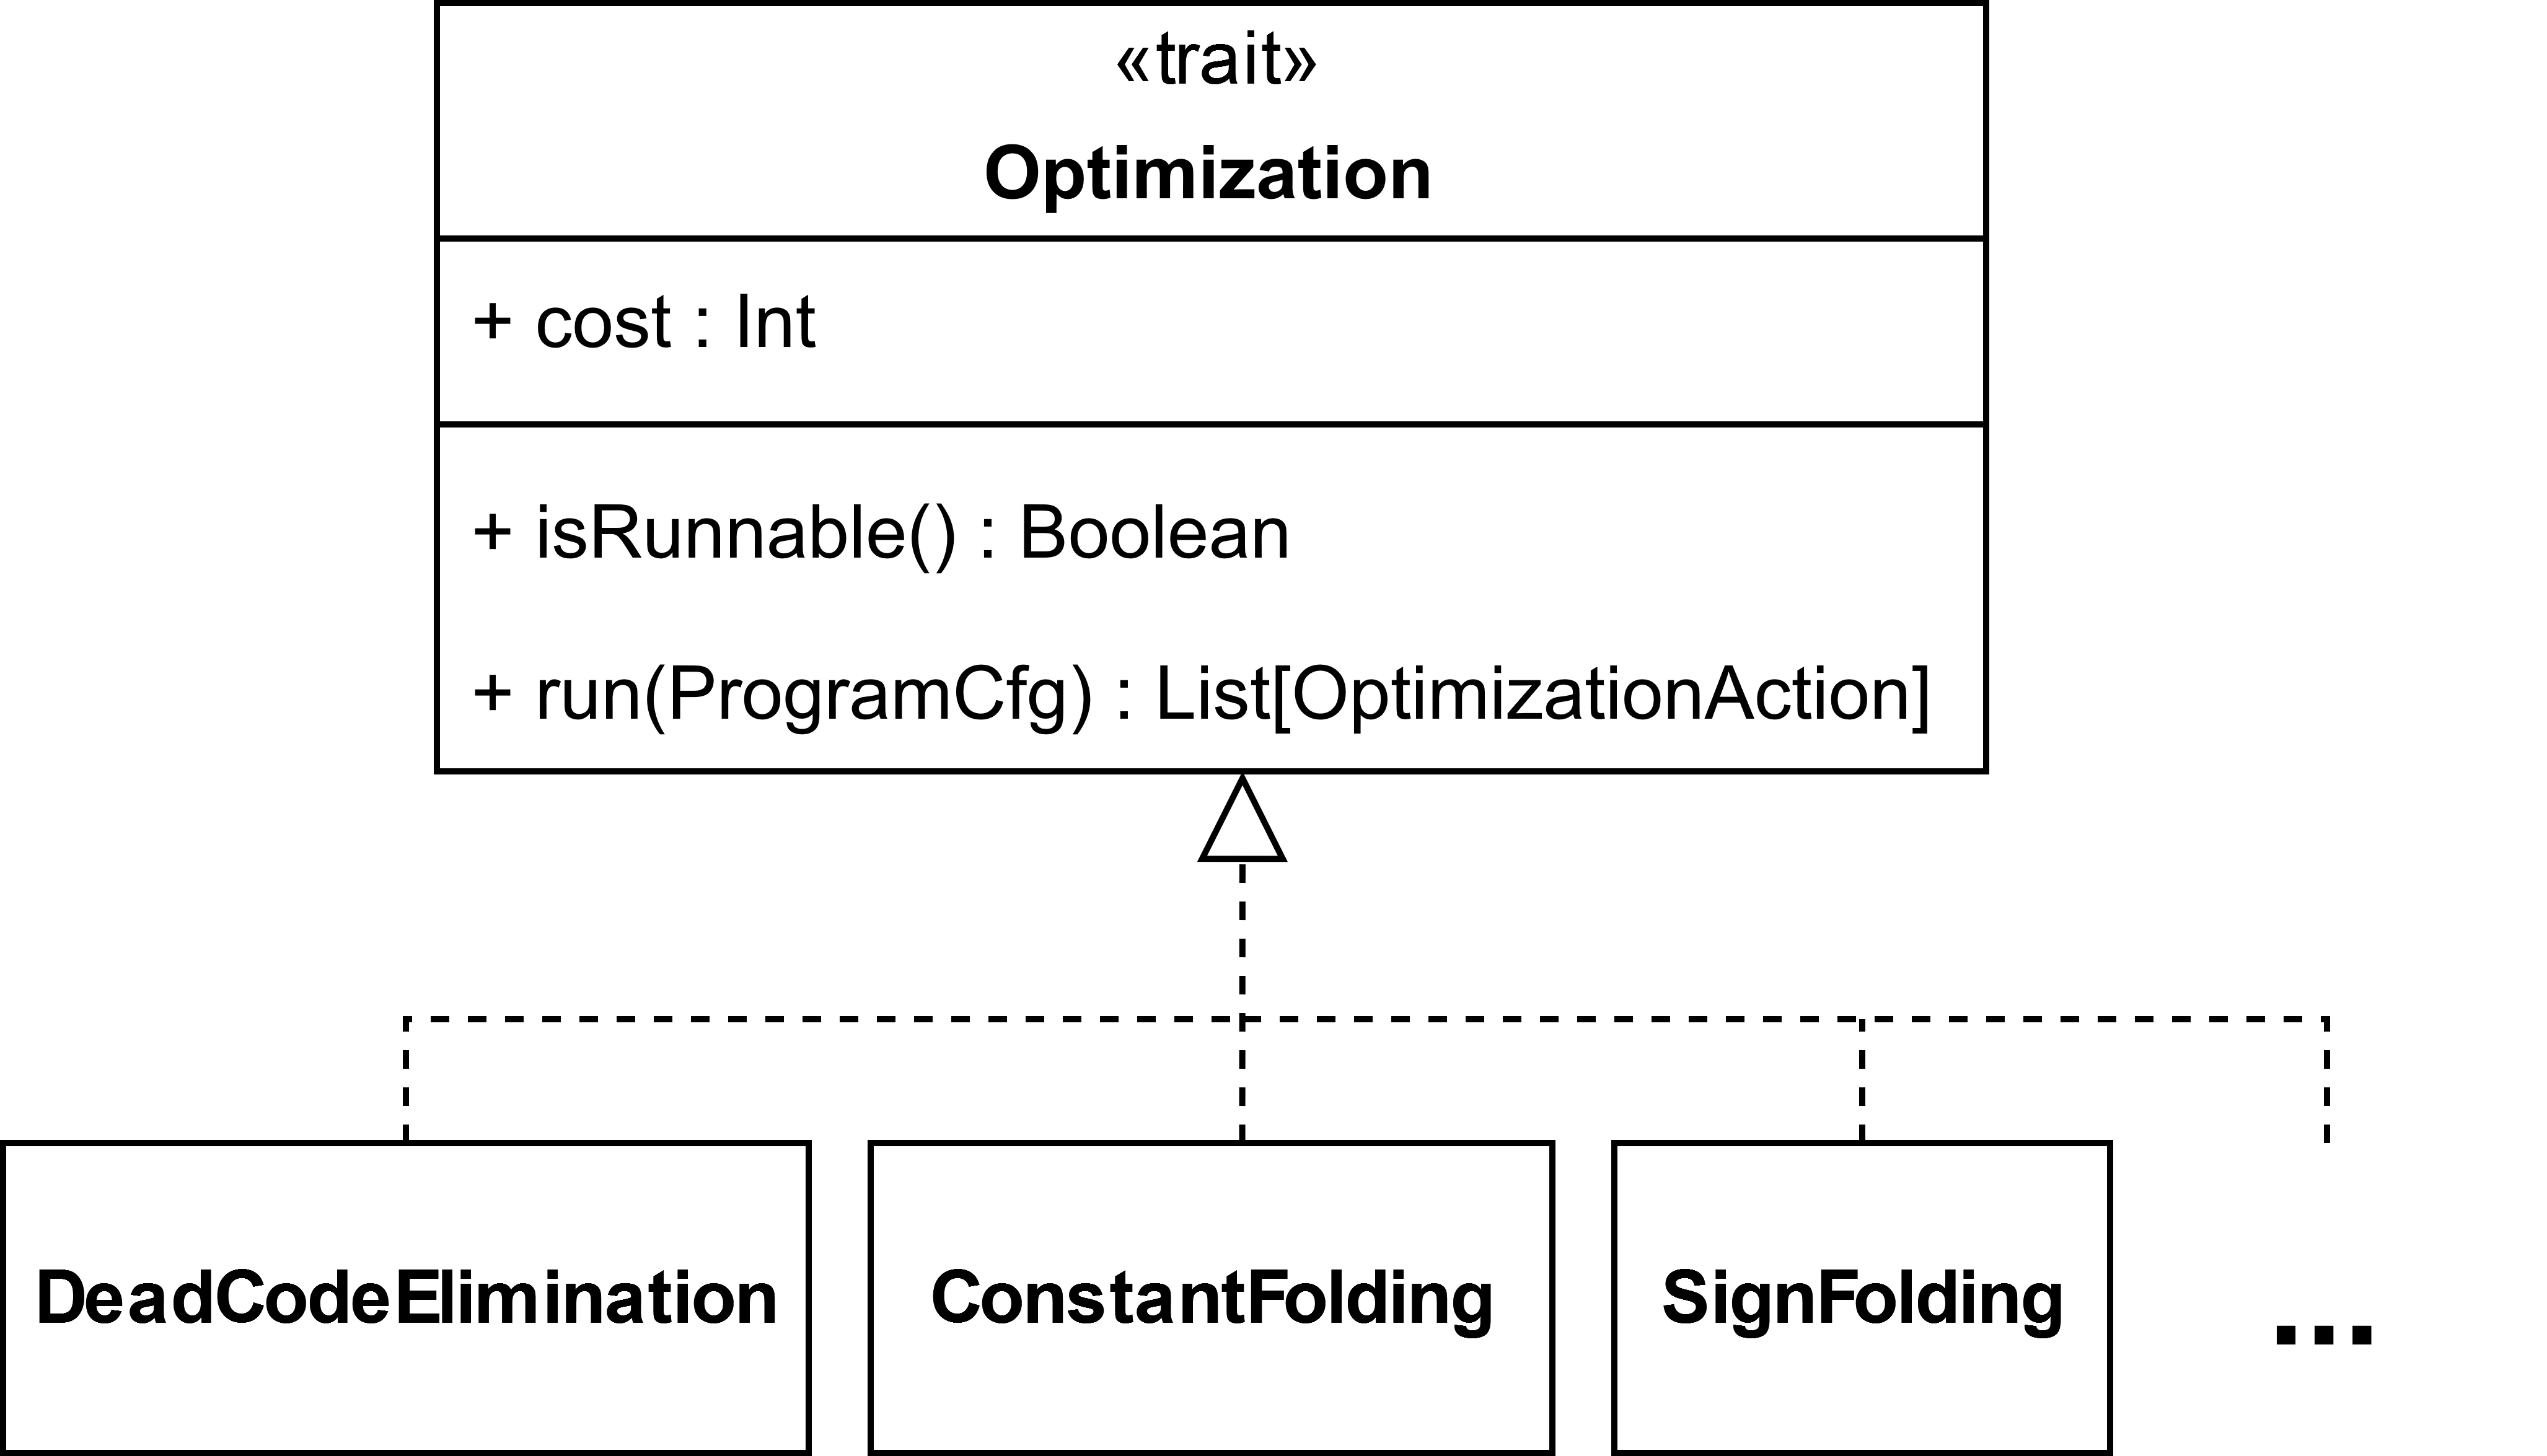
\includegraphics[height=5.5cm]{img/optimization_uml.png}
    \caption{UML class diagram of the optimization implementation.}\label{fig:optimization_uml}
\end{figure}


\subsection{Summary of the middleend}
In this section, we covered implementation of every component of the middleend. Now we encapsulate these components into a single class \texttt{Middleend} (see \autoref{lst:middleend_interface}) with arguments \texttt{AnalysisHandlerInterface} and \texttt{Language}. The second argument specifies the used microC language subset:
\begin{itemize}
    \item \texttt{microCVar}: basic microC constructs with no control flow
    \item \texttt{microCIf}: microCVar with if-statements
    \item \texttt{microCWhile}: microCIf with while-statements
    \item \texttt{microCFun}: microCWhile with function calls
    \item \texttt{microCRec}: microCFun with records
    \item \texttt{microCArr}: microCRec with arrays
    \item \texttt{microC}: entire microC language
\end{itemize}

The class has a single public method \texttt{astToCfg} which scans the input AST and throws an exception, if the AST contains constructs that are not part of the used microC subset. Then the AST is transformed into a CFG and optimized by the optimizer. The used budget of the optimizer depends on the argument \texttt{optimize}---if it is set to \texttt{true}, the budget is 500. Otherwise, the budget is 0 (meaning no optimization will be performed). The output of the method is a CFG and an instance of \texttt{AnalysesDb}.

\begin{listing}[H]
	\inputminted[tabsize=2,breaklines,bgcolor=codebg]{scala}{snippets/middleend_interface.m}
	\caption{The class \texttt{Middleend}.}
	\label{lst:middleend_interface}
\end{listing}

\section{The backend}
The last part of the compiler we will be implementing is the backend. As stated in \autoref{ssec:backend_design_summary}, our backend consists of 3 main components: \emph{CFG Compiler}, \emph{x86IR Compiler}, and \emph{Peepholer} (which will be sub-component of the \emph{x86IR Compiler}). In this section, we go over implementation of each of these components (and their subcomponents). The whole codebase of the backend is located in the folder \texttt{backend/}.

\subsection{x86IR}
The first part of \emph{x86IR Compiler} is x86IR itself, therefore in this subsection we go over its implementation. The implementation consists of the IR itself and builders of the IR, which are located in \texttt{x86IR/X86IR.scala} and \texttt{x86IR/X86IRBuilder.scala}, respectively.

\paragraph*{Type of instruction} The only common property of all instruction types is the byte-size, therefore we can model instruction type with a sealed trait \texttt{IRType} that defines single method \texttt{size}. The trait is then extended by:
\begin{itemize}
    \item \texttt{VoidType}---case object with size 0.
    \item \texttt{PointType}---case class with size 8 and argument \texttt{pointsTo} which defines the type it points to.
    \item \texttt{SimpleType}---case object with size 8.
    \item \texttt{ComposedType}---case class with size defined by the argument of the class.
\end{itemize}

\paragraph*{Instruction} As mentioned in \autoref{ssec:x86ir}, the common properties of all instructions are location and type. For the location we can reuse the class \texttt{Loc} defined in the codebase of AST and as for the type, we will use \texttt{IRType} defined earlier. For convenience purposes, we will also define common property \emph{operators}, which will be used to retrieve operands of the instruction in the live instruction analysis. We will model these properties with a sealed trait \texttt{Instruction}.

To distinguish terminating instructions from the non-terminating ones, we introduce yet another sealed trait called \texttt{Terminator}, which will extend \texttt{Instruction}. This trait will have a default type \texttt{VoidType} (since terminator instructions yield no value) and instructions \texttt{Return}, \texttt{CondJump}, and \texttt{Jump} will extend it. Every other instruction will extend the trait \texttt{Instruction} directly.

Each concrete instruction that directly or indirectly extends the trait \texttt{Instruction} is implemented as a case class. By doing so, we will be able to later implement their compilation using a pattern matching mechanism.

\paragraph*{Basic block} A basic block is a named sequence of instructions, which can be represented by a string (name of the basic block) and list of instructions. A basic block should also contain information about the origin of each of its instructions (the source CFG nodes). This information could be useful if, e.g., we wanted to reuse a result of some analysis provided by the middleend (which often maps properties of the program to CFG nodes). For this, we need an association between an instruction and its source CFG node, which can be defined as a map from \texttt{Instruction} to \texttt{CfgNode}. We model each of these properties with a case class \texttt{BasicBlock}.

Since the basic block is created step by step by adding instructions to it, we will use a builder pattern\footnote{\emph{Builder pattern} is used to simplify (often) multistep object creation by defining a class whose purpose is to build instances of another class \cite[Chap. 1]{java_pattern}.} to create it. We define a class \texttt{X86BbBuilder} which will have methods for adding instructions and building a basic block from the accumulated instructions. The builder will also prevent invalid actions like adding an instruction to a terminated basic block or building a non-terminated basic block by throwing an exception.

\paragraph*{Function} A function has a similar structure to a basic block, it can be represented by name, list of basic blocks, and number of parameters. Once again, these properties can be defined by a case class \texttt{Function}, which will also have methods for extracting local variables and arguments of the function.

When creating a function, we should keep track of already defined variables, so we can assign the correct memory address (represented by \texttt{Alloc} instruction) to each reference of a variable. This will be the responsibility of a builder class \texttt{X86FunctionBuilder}, which will also have methods for adding basic blocks and building a function from the accumulated basic blocks.

\paragraph*{The x86IR program} Finally, an x86IR program is a simple list of functions, modelled by a case class \texttt{ProgramX86IR} which also defines a method that returns the entry function of the program. The UML class diagram of the x86IR implementation is shown in \autoref{fig:x86IR_uml}.

We define yet another builder class \texttt{X86IRBuilder} which will serve as the main point for building an x86IR program. It will utilize the two builders for building basic blocks and functions we defined earlier on the background. Its main responsibility will be to switch contexts between the basic blocks and functions being built, while also making sure that each name of the created basic blocks is unique and there is no conflict with the names of functions\footnote{This would result in incorrect behaviour of jump instructions.}.

\begin{figure}
    \centering
    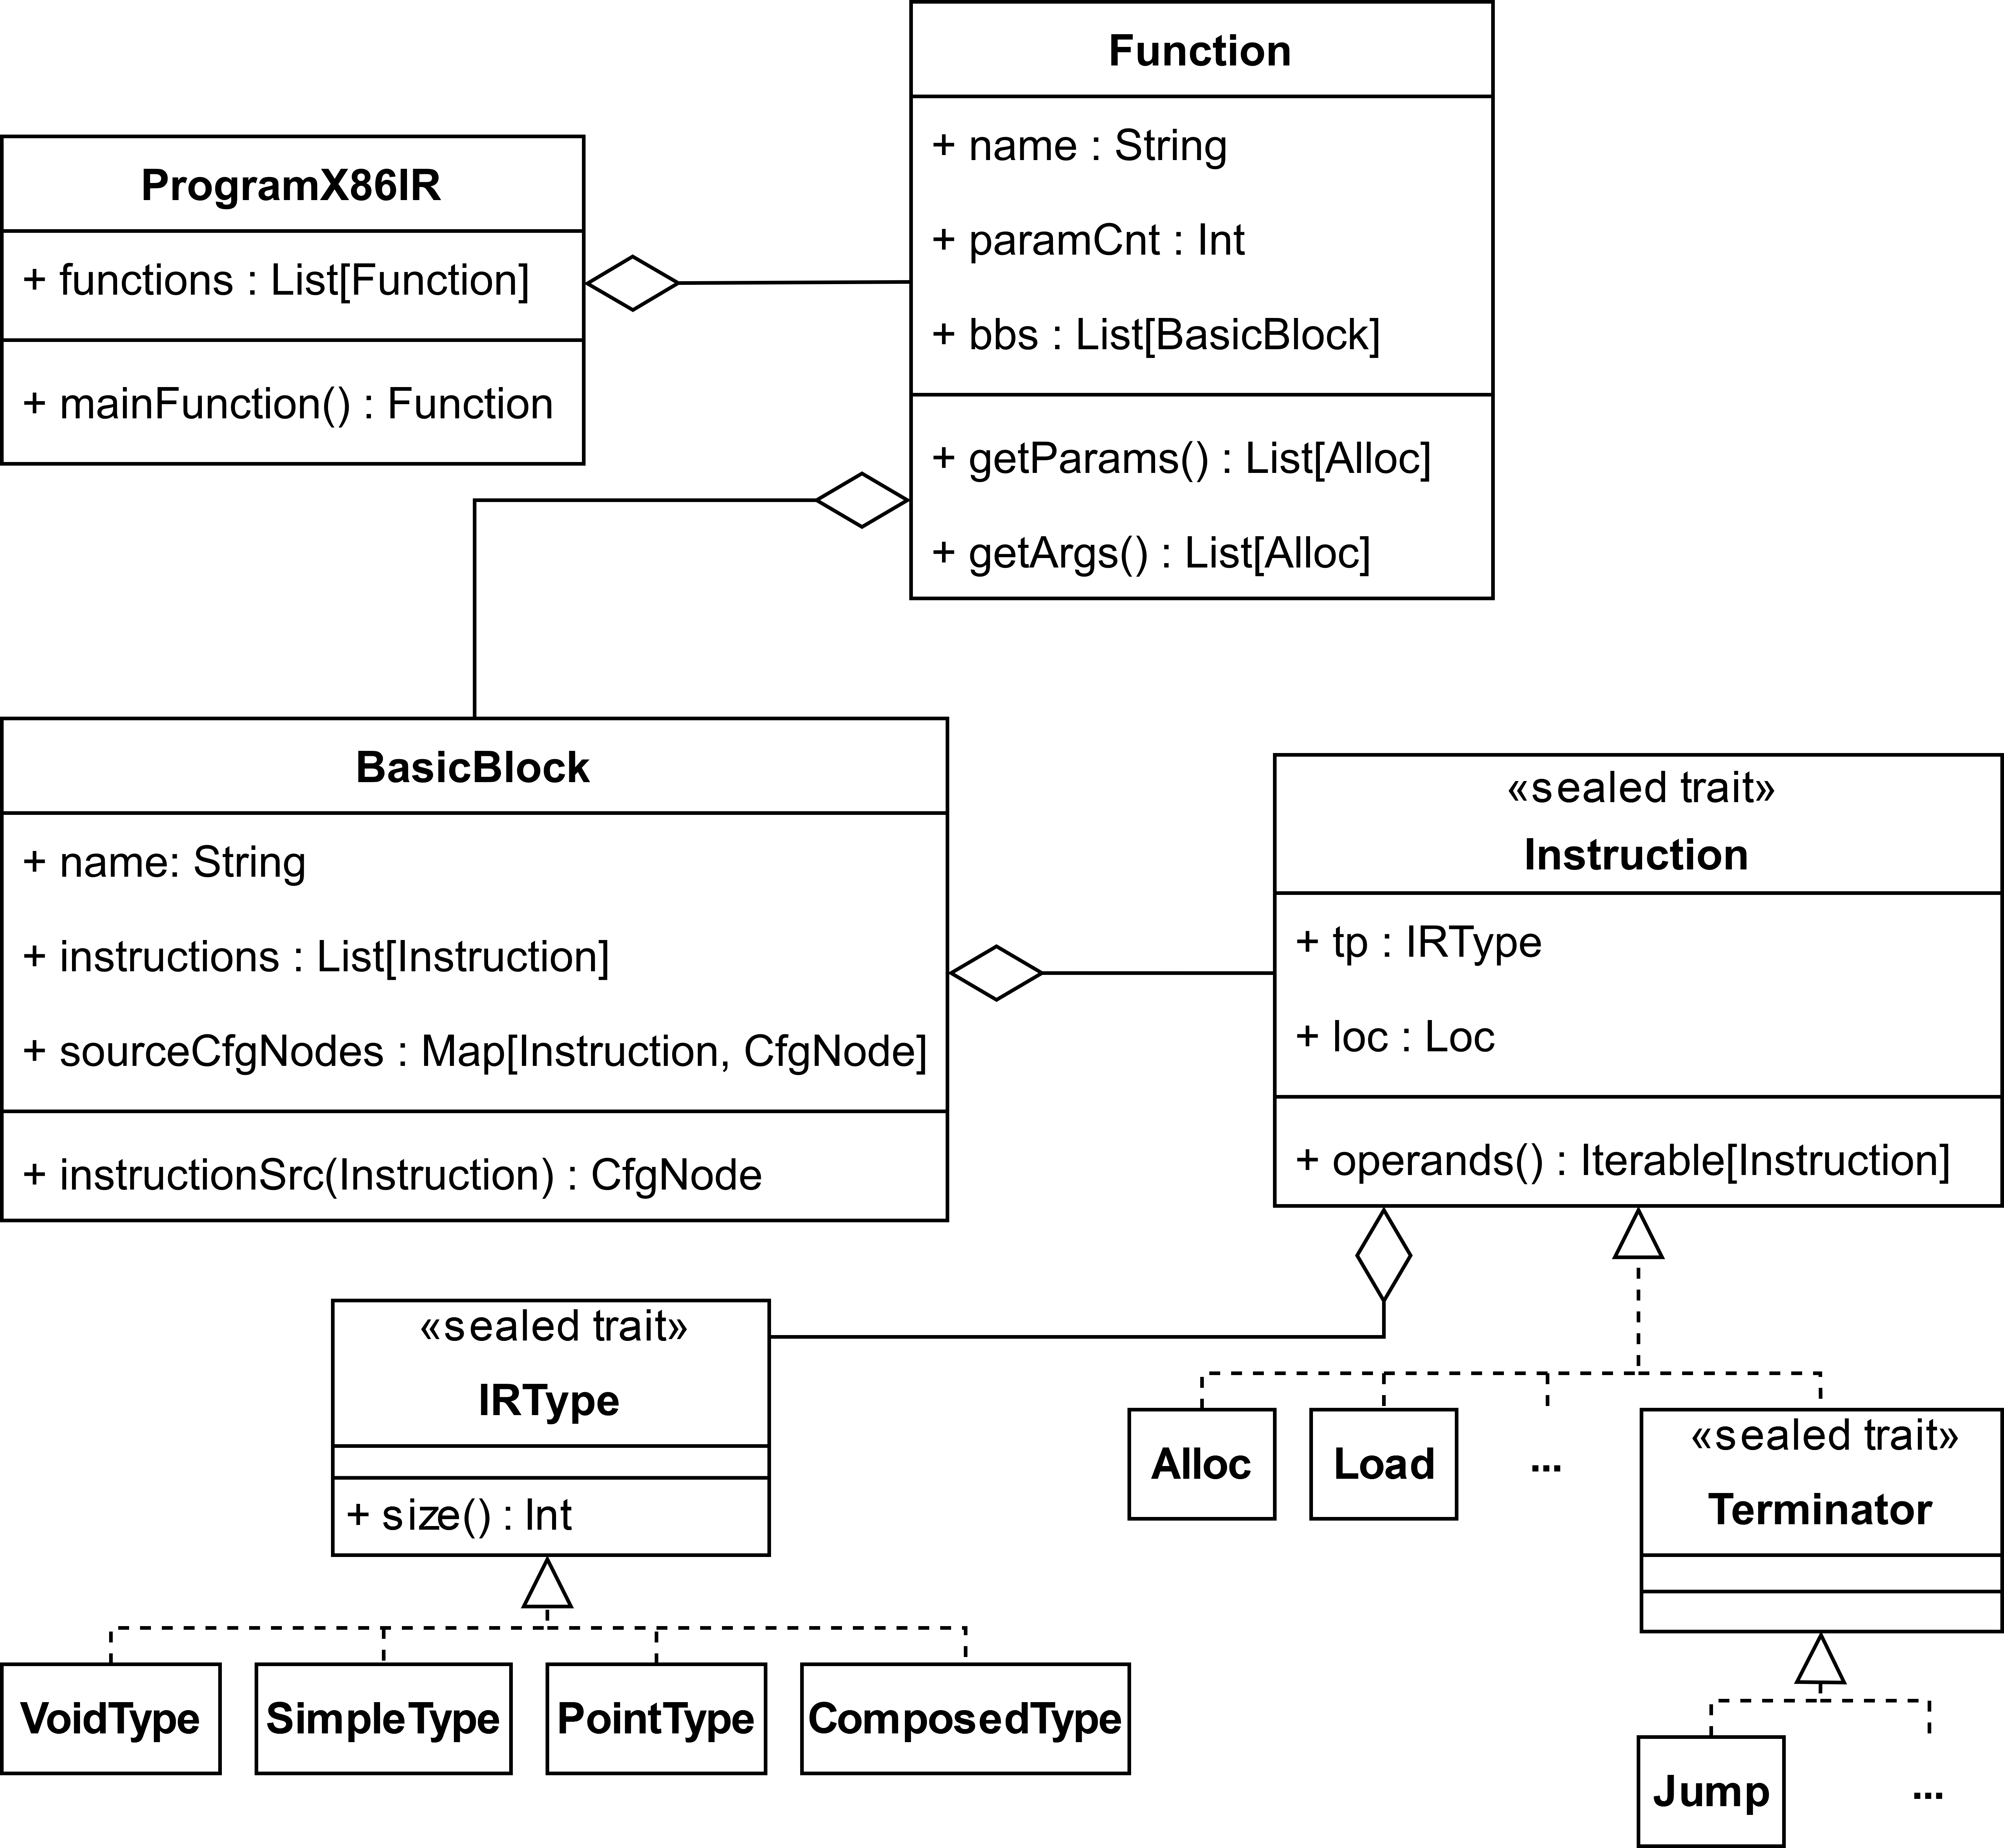
\includegraphics[height=11cm]{img/x86IR_uml.png}
    \caption{UML class diagram of the x86IR implementation.}\label{fig:x86IR_uml}
\end{figure}

\subsection{Code generation of x86IR}
With an implementation of the x86IR out of the way, we can finally introduce the class \texttt{CfgCompiler} (located in \texttt{x86IR/CfgCompiler.scala}). The arguments of the class are CFG of the program and results of type and semantic analysis (both of these are used to derive data types of expressions).

The class has a single public method \texttt{compile} which follows the compilation rules for each type of the CFG node we defined in \autoref{ssec:x86ir_gen} and builds an x86IR program by utilizing the builder class \texttt{X86IRBuilder} we defined in the previous subsection. Since the nodes are represented with case classes, we can simply use pattern matching for applying these rules.

In the last part of \autoref{ssec:x86ir_gen} we decided to implement field access using an offset from the address of the record. Since the size of this offset depends on the type of record's members, we have to somehow derive their types. For this purpose we define a helper class \texttt{TypeAnalyzer} (located in \texttt{x86IR/TypeAnalyzer.scala}) which by utilizing the results of type and semantic analysis will derive the correct \texttt{IRType} of expressions.

\subsection{x86 assembly}
To be able to compile x86IR to x86 assembly, we need to define a program representation of the assembly. The representation should be easily serializable while also allowing to perform peephole optimizations by applying the rewrite rules defined in \autoref{tab:peephole_rules}. In this subsection, we go over such representation. Its implementation, formatter, and builder are located in \texttt{x86/helper/}, \texttt{x86/X86Formatter}, and \texttt{x86/X86Builder.scala}, respectively.

\paragraph*{Instruction representation} When it comes to the shape of the instructions we will be using, we can divide them into 3 types:
\begin{enumerate}
    \item Zero operand instructions: \texttt{name} (e.g., \texttt{ret})
    \item One operand instructions: \texttt{name op1} (e.g., \texttt{inc} or \texttt{dec})
    \item Two operand instructions: \texttt{name op1, op2} (e.g., \texttt{mov} or \texttt{add})
\end{enumerate}

The only common property of these types is the name of the instruction, therefore we will represent an x86 instruction with a sealed trait \texttt{Instruction} extended by 3 sealed traits representing each of the shape types, as shown in \autoref{fig:x86instruction_uml}. Thanks to this representation, the formatter (which will handle the serialization) will not have to define serialization for each instruction separately, but only for these 3 traits. For convenience purposes, the trait \texttt{Instruction} will also allow to optionally assign a comment to an instruction.

To be able to use pattern matching for applying rewrite rules on instructions in the peepholer, we define each concrete instruction as a case class. Similarly, the operands of the instructions (registers, memory accesses, labels, and immediate values) will be represented with case objects and case classes, extending a sealed trait \texttt{Operand}.

\begin{figure}
    \centering
    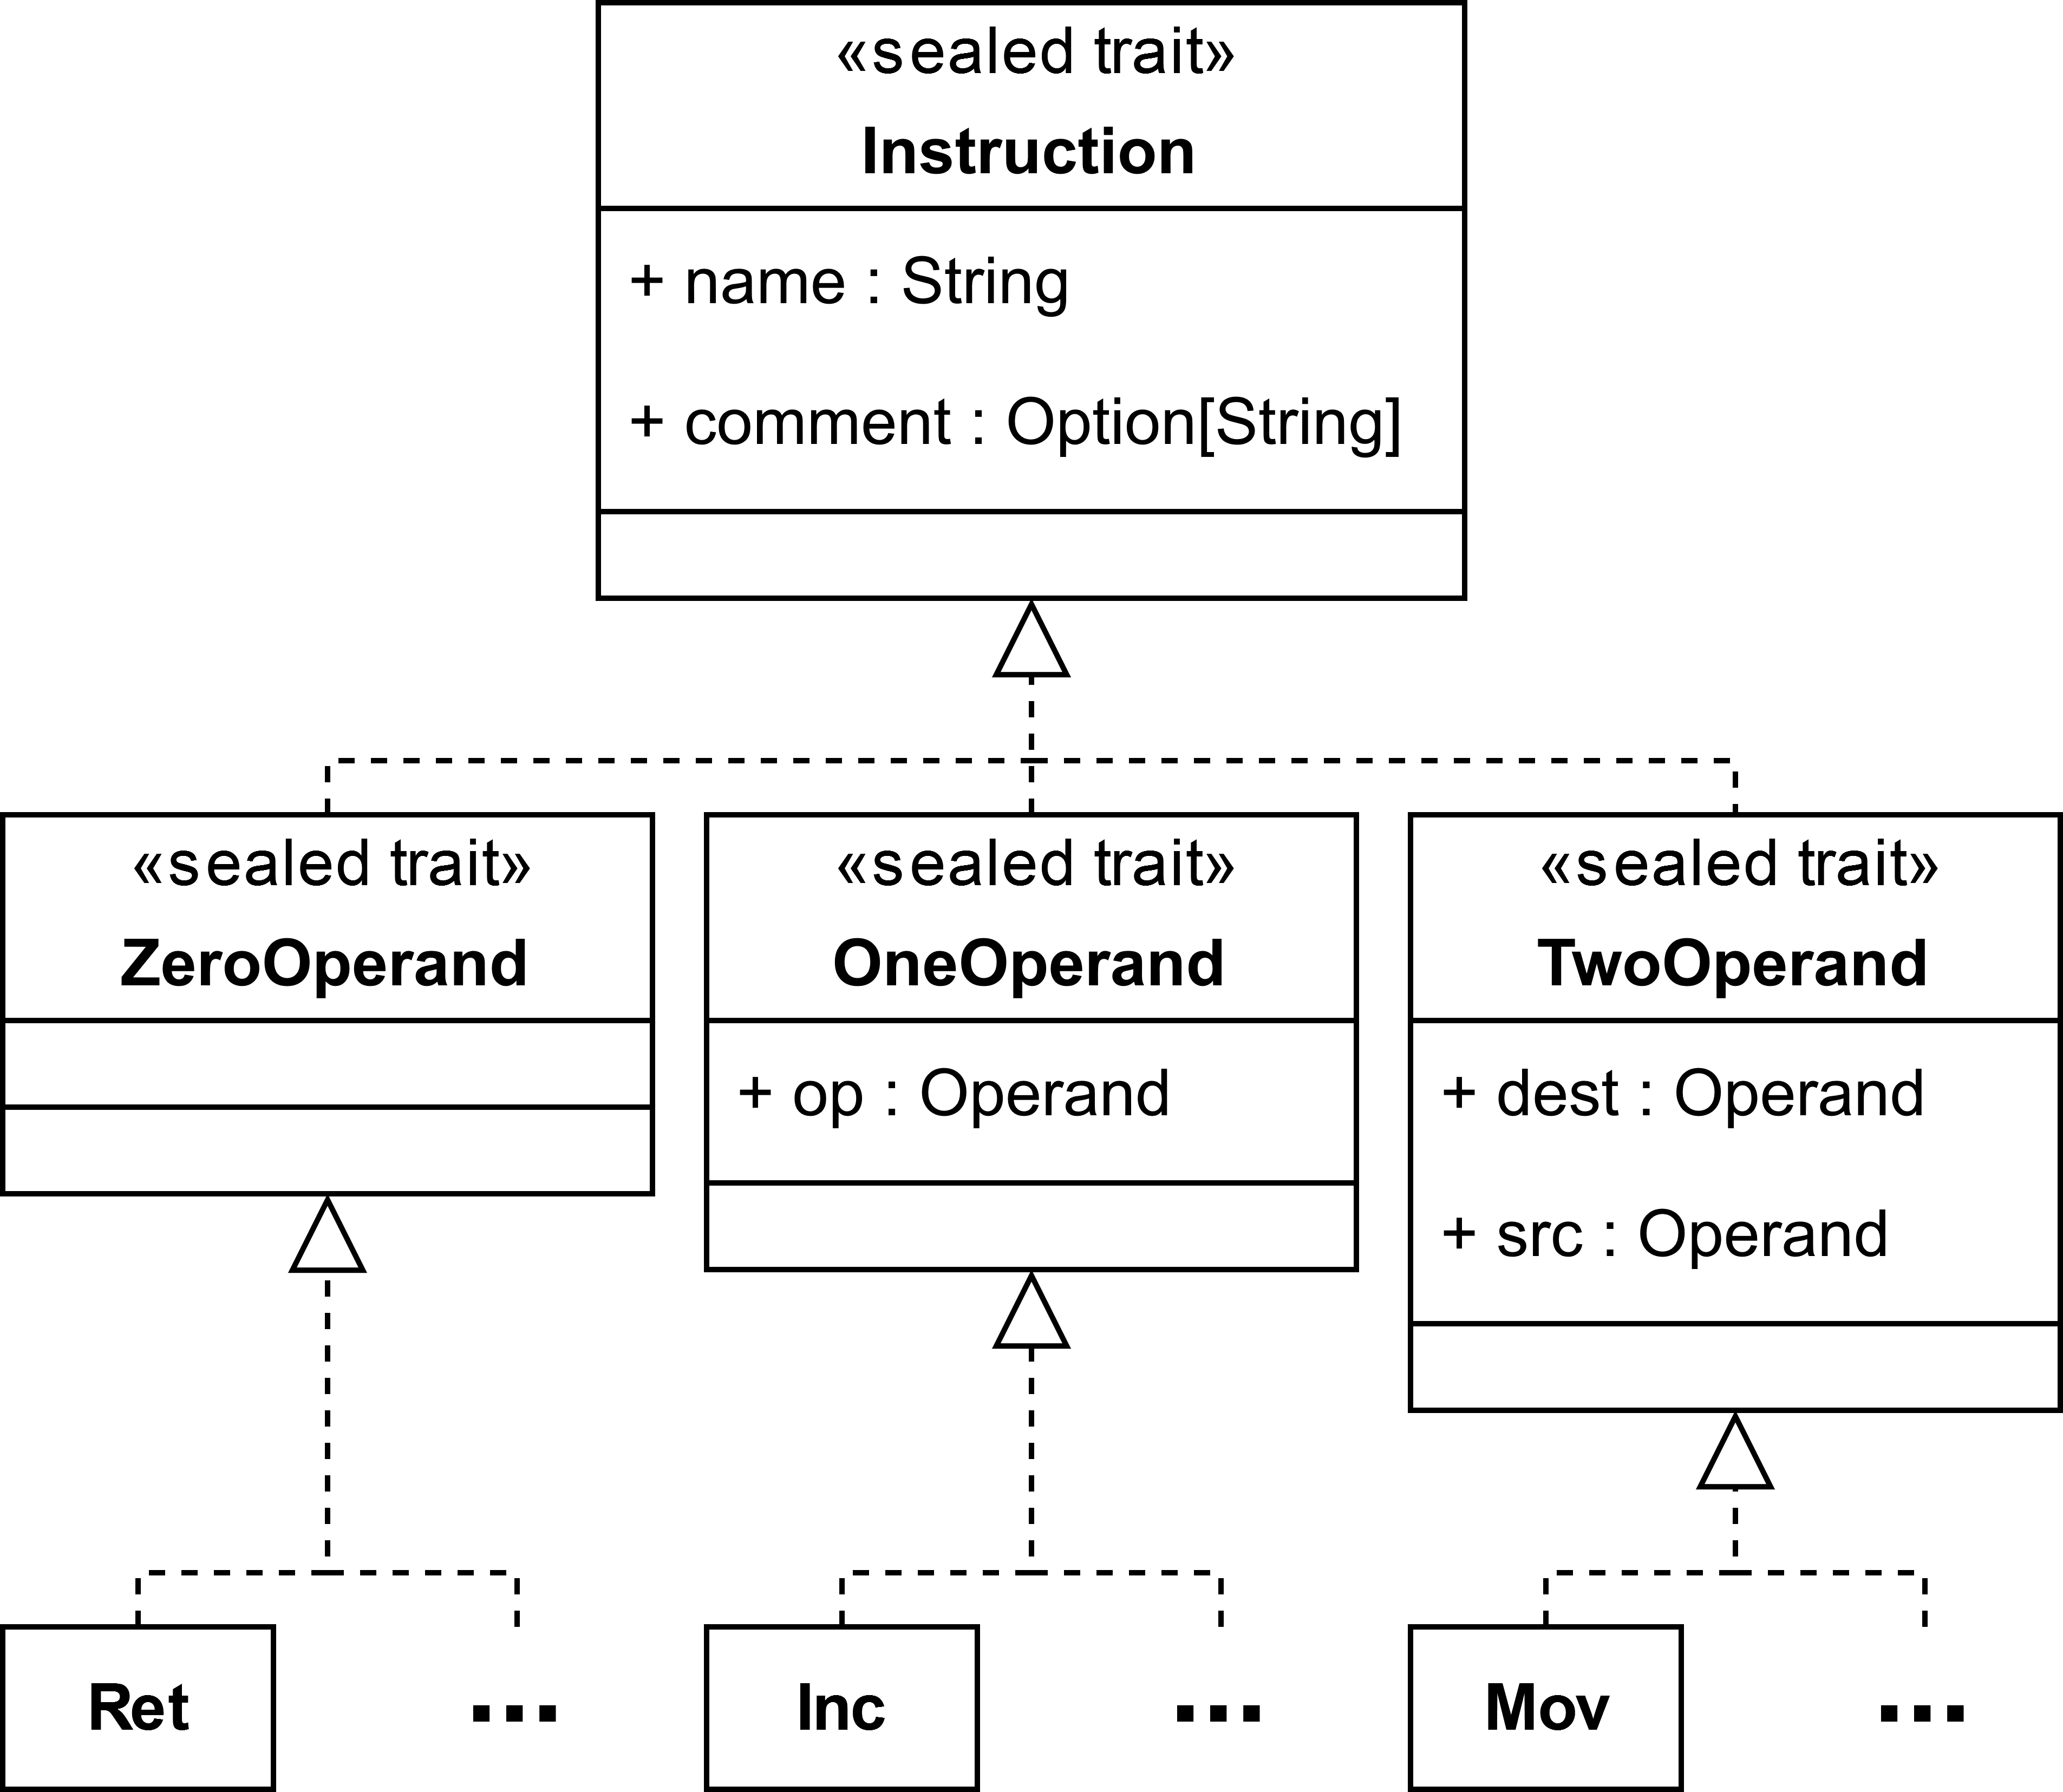
\includegraphics[height=6.5cm]{img/instruction_uml.png}
    \caption{UML class diagram of the x86 instruction implementation.}\label{fig:x86instruction_uml}
\end{figure}

\paragraph*{Formatter} The serialization of the instruction depends on the used syntax of x86 assembly, which often differs in order or format of the instruction operands. An example of these differences is shown in \autoref{lst:x86syntax_comparsion}, which compares NASM\footnote{Netwide Assembler: \url{https://www.nasm.us/}} syntax and GAS\footnote{GNU Assembler: \url{https://www.gnu.org/software/binutils/}} syntax.

\begin{listing}[H]
\centering
\begin{minipage}{.4\linewidth}
	\inputminted[tabsize=2,breaklines,bgcolor=codebg]{nasm}{snippets/nasm.m}
\end{minipage}%
\hskip0.2cm
\begin{minipage}{.5\linewidth}
	\inputminted[tabsize=2,breaklines,bgcolor=codebg]{gas}{snippets/gas.m}
\end{minipage}%
	\caption[Comparison of NASM and GAS syntax.]{Comparison of NASM (on the left) and GAS (on the right) syntax.}
	\label{lst:x86syntax_comparsion}
\end{listing}

To ensure extensibility of supported syntaxes, it is better to define a separate class (or in our case, a trait) for instruction formatting and serialization. Therefore, we introduce a trait \texttt{X86Formatter}, which defines methods for formatting instructions and their operands. We also introduce an object \texttt{NasmFormatter} which extends the trait and implements formatting of the NASM syntax. The support for another syntaxes is simply added by extending the trait.

\paragraph*{Builder} We will produce x86 assembly using the builder class \texttt{X86Builder}, which accumulates instructions into a list until \texttt{build} method is called. Then the builder may apply peephole optimizations to the instruction list by using the \texttt{Peepholer} class, which we will discuss in the following subsection. Finally, each instruction is serialized using the formatter which we defined earlier.

\subsection{Peepholer}\label{ssec:peepholer}
We implement peepholer as a stateless object \texttt{Peepholer} with a single public method \texttt{optimize} that repeatedly applies peephole optimizations on a list of instructions until a fixed point is reached. The sliding window can be implemented by a recursive function that observes one or two instructions at a time and applies rewrite-rules from \autoref{tab:peephole_rules} using a pattern matching\footnote{This is where the representation of instructions and their operands as case objects and case classes comes in handy, since they come with syntactic conveniences for pattern matching generated by the compiler \cite[Chap. 15]{scala}.}. The output of the peepholer will be an optimized list of instructions. The implementation is located in \texttt{x86/Peepholer.scala}.

\subsection{Live instruction analysis}
The goal of the live instruction analysis is to decide which values are live after execution of the given instruction (recall \autoref{ssec:lia}). We define a class \texttt{LiveInstructionAnalysis} which performs the analysis, stores the result, and gives access to the result. The class is located in folder \texttt{x86/}.

The class will perform the analysis upon its creation by analysing each basic block of the x86 program. Since the recurrence relation of the analysis (see \autoref{ssec:lia}) is defined from the last instruction of the basic block, we will do this by iterating over the list of instruction in reverse and applying the relation rules. The result of the analysis will be a map that maps each instruction of the basic block to a set of instructions whose value is live. Access to this result will be provided by a method \texttt{liveAfterInstr}, which for the given basic block and instruction returns a set of instructions whose value is live after the given instruction.

In addition, the class will also store the order in which the results of instructions will be used as operands of some other instruction. This will be useful information for the register allocation we will be discussing in the following subsection. Access to this order is provided by the method \texttt{usageOrder}.

\subsection{Compiler memory}
To be able to map x86IR to x86 assembly, we will need to somehow simulate the memory of the x86 target machine, since the compiler needs to keep track of which instruction results are assigned to which registers or which memory offsets are assigned to which local variables. Another responsibility of the compiler will be to decide which values should reside in registers and which in memory (this process is called a \emph{register allocation} \cite[Chap. 11.2]{eng_comp}). Therefore, we introduce a class \texttt{CompilerMemory} (located in \texttt{x86/CompilerMemory.scala}) which will simulate the x86 machine memory and perform a register allocation.

\paragraph*{Memory representation} The function frame stack is represented by two member variables. The first one, \texttt{variables}, represents the part of the stack that contains local variables and arguments of the function. It is a map that maps these values to offsets which have been assigned to them by the methods \texttt{addLocal} and \texttt{addArg}. The second one, \texttt{temps}, represents the part of the stack that contains temporary values (e.g., fields of a record). It is a map that maps these values to their offsets assigned by the method \texttt{allocateTempOnStack}.

Registers of the x86 machine are represented by the variable \texttt{registers}, which maps the registers to values they contain (an instance of \texttt{Option}\footnote{The class \texttt{Option} is a container for zero or one element of a given type. Instances of \texttt{Option} are either \texttt{Some} (single element) or \texttt{None} (no element) \cite{option}.}). The values are assigned to registers via the method \texttt{allocReg}, which performs the register allocation process.

\paragraph*{Register allocation} The method \texttt{allocReg} performs the register allocation for a value by finding an empty register. If no register is empty, it selects a register with a value that will be used furthest in the future and spills it onto the stack. To decide which value will be used furthest in the future, the method uses the class \texttt{LiveInstructionAnalysis}, which gives access to the order in which the results of instructions are used.

The method \texttt{load} is used to return the register in which the given value is stored. If the value is stored on the stack, it is moved from the stack into an empty register. If no register is empty, the method performs the same spilling process as the method \texttt{allocReg}.


\subsection{Code generation of x86 assembly}
The last component implementation we will be discussing in this section is the class \texttt{X86IRCompiler} (located in \texttt{x86/X86IRCompiler.scala}). The arguments of the class are x86IR program, syntax of the output x86 assembly, and a boolean which determines whether the peephole optimizations should be applied.

The generation of x86 assembly is performed by the method \texttt{compile}, which utilizes the classes we discussed earlier (\texttt{X86Builder}, \texttt{CompilerMemory}, and \texttt{LiveInstructionAnalysis}). Since the x86IR is modelled with the usage of case classes, the compilation process we described in \autoref{ssec:x86_code_gen} is implemented by using a pattern matching (similarly as in the code generation of x86IR).

\subsection{Summary of the backend}
The last step of backend implementation will be to encapsulate both components \texttt{CfgCompiler} and \texttt{X86IRCompiler} into a single class representing the backend of the microC compiler. However, before we do that, we will first define a general interface of the microC backend, since in the future more types of backend can be implemented (e.g., a backend that compiles CFG into JVM\footnote{Java Virtual Machine} bytecode). This interface is modelled by a trait \texttt{Backend} with a single public method \texttt{compile}, which takes \texttt{ProgramCfg} (CFG of the program), \texttt{AnalysesDb} (results of analyses of the program), boolean \texttt{optimize} (determining if the backend should perform optimizations) and returns the target language program representation.

Finally, this interface is implemented by the class \texttt{X86Backend}, which puts together and encapsulates both components \texttt{CfgCompiler} and \texttt{X86IRCompiler}. The class \texttt{X86Backend} is shown in \autoref{lst:backend_interface} together with the trait \texttt{Backend}.

\begin{listing}[H]
	\inputminted[tabsize=2,breaklines,bgcolor=codebg]{scala}{snippets/backend_interface.m}
	\caption{The trait \texttt{Backend} and its implementation for the x86 backend.}
	\label{lst:backend_interface}
\end{listing}

\section{Summary of the compiler}
The obvious last step of the compiler implementation is to put all three “pieces of the puzzle” (frontend, middleend, and backend) together. This is done by the class \texttt{Compiler} (see \autoref{lst:compiler_interface}) which encapsulates the whole codebase of the microC compiler. Its usage is described in detail in \autoref{sec:how_to_use}.

\begin{listing}[H]
	\inputminted[tabsize=2,breaklines,bgcolor=codebg]{scala}{snippets/compiler_interface.m}
	\caption{The class \texttt{Compiler}.}
	\label{lst:compiler_interface}
\end{listing}

This concludes implementation of the microC compiler. The size of the compiler codebase and each of its parts is shown in \autoref{tab:implementation_overview}. Part of the codebase are also example implementations of each analysis covered in \autoref{sec:analyses}. For a detailed manual how to use the compiler or how to run programs produced by the compiler, see \autoref{chap:manual}.

\begin{table}[h]
\centering
\begin{tabular}{|l||l|l|}
\hline
& \makecell{Number of code lines (without \\ empty lines and comments)} & \makecell{Number of classes, \\ traits, and objects}\\
\hline
\hline
Frontend & 7 & 1\\
\hline
Middleend & 1509 & 54\\
\hline
Backend & 1540 & 116\\
\hline
Whole codebase & 3101 & 175\\
\hline
\end{tabular}
\caption{Size of the compiler codebase without the NI-APR codebase.}
\label{tab:implementation_overview}
\end{table}


\section{Testing}
The project uses two types of tests---unit tests and black-box tests. We will discuss each of these tests in the next two subsections. Both of these tests are also part of a continuous integration managed by GitLab (where the project's codebase is hosted). With each push or merge request, GitLab runs a pipeline of scripts that will build the project and run both of the mentioned tests. The pipeline is defined in a file \texttt{.gitlab-ci.yml} located in the root of the project.

\subsection{Unit tests}
Unit testing involves testing software code at its smallest functional point, which is typically a single class \cite[Chap. 3.4.5]{testing}. The project contains over 90 unit tests (with over 2000 lines of code) which cover every major class discussed in the previous sections of this chapter. Tests are located in \texttt{microc-compiler/src/test/scala/microc} and use a library called \emph{uTest}\footnote{\url{https://github.com/com-lihaoyi/utest}}.

Library \emph{uTest} provides a simplistic codebase and functionality for defining test suites and running tests. A test suite is defined by extending abstract class \texttt{TestSuite} as shown in \autoref{lst:test_suite}, which is an example of a test suite for the class \texttt{Peepholer}. Tests can be run from the folder \texttt{microc-compiler} via command \texttt{sbt test}.

\begin{listing}[H]
	\inputminted[tabsize=2,breaklines,bgcolor=codebg]{scala}{snippets/test_suite.m}
	\caption{Example of a test suite.}
	\label{lst:test_suite}
\end{listing}

\subsection{Black-box tests}
Unlike the unit testing, the black-box testing involves testing of a software code where the inner program structure of the code is not pertinent. The test design is based strictly on the expected program functionality \cite[Chap. 8.2.2]{testing} (in our case, what output should be produced by the input microC program compiled by our compiler).

The tests are run from the folder \texttt{test} via script \texttt{./test.sh}. The script compiles and runs every microC program in the folder \texttt{test/in} (there are over 30 test programs) and compares their outputs with the reference outputs located in the folder \texttt{test/ref}. For each program, both optimized and unoptimized versions are run.


\section{Documentation}
Since this project should serve as an educational material, it is important to provide a proper documentation of the project's code-base. The project uses the system \emph{Scaladoc}\footnote{\url{https://docs.scala-lang.org/style/scaladoc.html}}, which is the most common document generation system for Scala source codes. \emph{Scaladoc} reads specially formatted comments called \emph{annotations} in Scala source code (see \autoref{lst:annotation} for an annotated source code example) and generates compiled HTML documentation. \emph{Scaladoc} annotations are also recognized by most of the popular IDEs like IntelliJ IDEA, Visual Studio Code, or Eclipse which offer tools like auto-complete, detection of non-matching annotations, etc.

Documentation can be generated from the folder \texttt{microc-compiler} via command \texttt{sbt doc}. After running the command, the documentation can be typically found in a folder \texttt{microc-compiler/target/scala-X.XX/api}, where “X.XX” depends on the version of Scala. For an example of a generated documentation of the class \texttt{Compiler}, see \autoref{fig:documentation}.

\begin{listing}
	\inputminted[tabsize=2,breaklines,bgcolor=codebg]{scala}{snippets/annotation.m}
	\caption{Annotation of the class \texttt{Optimizer}.}
	\label{lst:annotation}
\end{listing}

\begin{figure}
    \centering
    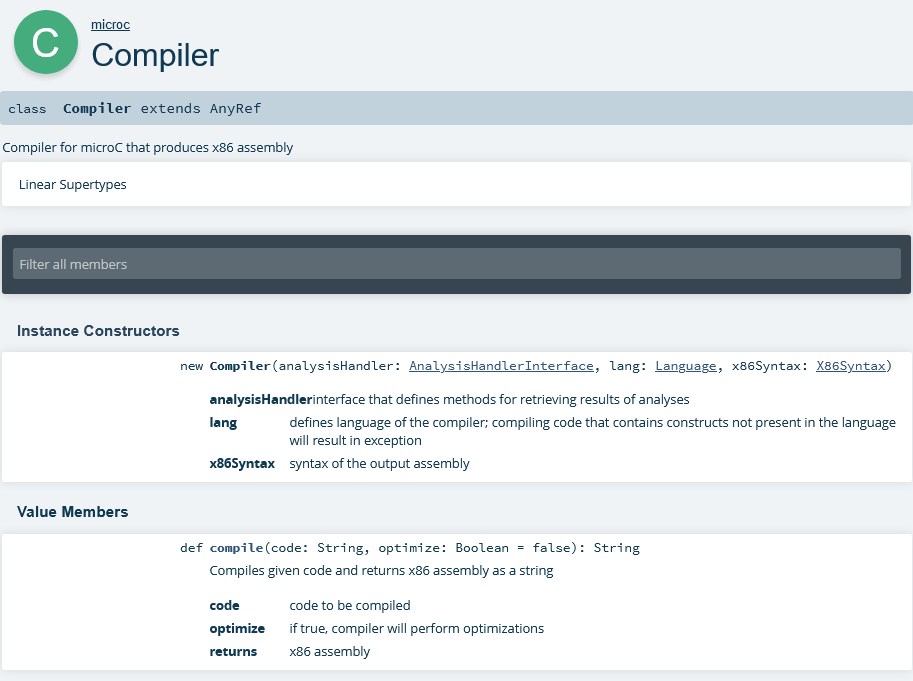
\includegraphics[width=12.5cm]{img/documentation.png}
    \caption{Generated documentation of the class \texttt{Optimizer}.}\label{fig:documentation}
\end{figure}



\chapter{Assessment}
In this chapter, we demonstrate the effects of optimizations performed by our compiler by going over the optimization process of three example programs (or, to be precise, functions), step-by-step and compare the produced assembly code before and after optimizations. In the last example, we will also compare the produced assembly code with the one produced by GCC by compiling an equivalent program written in C.

\section{Example 1}\label{sec:optim_ex1}
Let us consider following function:
\begin{minted}[tabsize=2,breaklines,linenos,escapeinside=||]{python}
foo(in) {
	|\microcvar| x, y, z;
	x = 60 * 24;
	y = x * in;
	if (x > 1400) {
		z = y + 10;
	} else {
		z = y - 10;
	}
	return z;
}
\end{minted}

Assembly code generated by compiling this function without any optimization is shown in \autoref{lst:foo_before}. At first glance, it is obvious, that this function can be optimized. Without any analysis provided, the compiler will perform the constant folding optimization on the binary operation on line 3:
\pagebreak

\begin{minted}[tabsize=2,breaklines,linenos,escapeinside=||]{python}
foo(in) {
	|\microcvar| x, y, z;
	x = 1440;
	y = x * in;
	if (x > 1400) {
		z = y + 10;
	} else {
		z = y - 10;
	}
	return z;
}
\end{minted}

At this point, no further optimization can be performed by the compiler without providing more information about the function. One way to do that is to provide the constant propagation analysis to the compiler. The result of this analysis for function \texttt{foo} looks like this:

\begin{align*}
    [\![ \emph{entry} ]\!] &= \{ x \rightarrow \bot, y \rightarrow \bot, z \rightarrow \bot, in \rightarrow \top \}\\
    [\![ \texttt{var x, y, z} ]\!] &= \{ x \rightarrow \bot, y \rightarrow \bot, z \rightarrow \bot, in \rightarrow \top \}\\
    [\![ \texttt{x = 1440} ]\!] &= \{ x \rightarrow 1440, y \rightarrow \bot, z \rightarrow \bot, in \rightarrow \top \}\\
    [\![ \texttt{y = x * in} ]\!] &= \{ x \rightarrow 1440, y \rightarrow \top, z \rightarrow \bot, in \rightarrow \top \}\\
    [\![ \texttt{x > 1400} ]\!] &= \{ x \rightarrow 1440, y \rightarrow \top, z \rightarrow \bot, in \rightarrow \top \}\\
    [\![ \texttt{z = y + 10} ]\!] &= \{ x \rightarrow 1440, y \rightarrow \top, z \rightarrow \top, in \rightarrow \top \}\\
    [\![ \texttt{z = y - 10} ]\!] &= \{ x \rightarrow 1440, y \rightarrow \top, z \rightarrow \top, in \rightarrow \top \}\\
    [\![ \texttt{return z} ]\!] &= \{ x \rightarrow 1440, y \rightarrow \top, z \rightarrow \top, in \rightarrow \top \}\\
    [\![ \emph{exit} ]\!] &= \{ x \rightarrow 1440, y \rightarrow \top, z \rightarrow \top, in \rightarrow \top \}\\
\end{align*}

With this knowledge, the compiler can now replace variable \texttt{x} on lines 4 and 5 with a constant $1440$ by performing the constant propagation optimization:

\begin{minted}[tabsize=2,breaklines,linenos,escapeinside=||]{python}
foo(in) {
	|\microcvar| x, y, z;
	x = 1440;
	y = 1440 * in;
	if (1440 > 1400) {
		z = y + 10;
	} else {
		z = y - 10;
	}
	return z;
}
\end{minted}

This optimization enables once again the constant folding optimization, which folds the comparison operator on line 5:

\begin{minted}[tabsize=2,breaklines,linenos,escapeinside=||]{python}
foo(in) {
	|\microcvar| x, y, z;
	x = 1440;
	y = 1440 * in;
	if (1) {
		z = y + 10;
	} else {
		z = y - 10;
	}
	return z;
}
\end{minted}

The next optimization the compiler will perform here is obvious---since the guard of the if-statement on line 5 always evaluates to true, the compiler will eliminate the whole if-statement and replace it with the \emph{then} branch by performing the dead code elimination:

\begin{minted}[tabsize=2,breaklines,linenos,escapeinside=||]{python}
foo(in) {
	|\microcvar| x, y, z;
	x = 1440;
	y = 1440 * in;
	z = y + 10;
	return z;
}
\end{minted}

Once again, the compiler reaches the point where it cannot perform any optimization, not even with the constant propagation analysis, since no variable can be propagated anymore. However, in this situation, the compiler could benefit from a result of the live variable analysis, which gives information about live variables at each point of the program. In case of the function \texttt{foo}, the result of the analysis looks like this:

\begin{align*}
    [\![ \emph{entry} ]\!] &= \{ in \}\\
    [\![ \texttt{var x, y, z} ]\!] &= \{ in \}\\
    [\![ \texttt{x = 1440} ]\!] &= \{ in \}\\
    [\![ \texttt{y = 1440 * in} ]\!] &= \{ in \}\\
    [\![ \texttt{z = y + 10} ]\!] &= \{ y \}\\
    [\![ \texttt{return z} ]\!] &= \{ z \}\\
    [\![ \emph{exit} ]\!] &= \emptyset\\
\end{align*}

As we can see, at no point in the function \texttt{foo} is the variable \texttt{x} live. The compiler will use this information to eliminate the assignment on line 3 by performing the dead statement elimination:

\begin{minted}[tabsize=2,breaklines,linenos,escapeinside=||]{python}
foo(in) {
	|\microcvar| x, y, z;
	y = 1440 * in;
	z = y + 10;
	return z;
}
\end{minted}

Since the variable \texttt{x} is no longer used anywhere in the function \texttt{foo}, the compiler will perform the unused variable elimination and remove the declaration of variable \texttt{x}:

\begin{minted}[tabsize=2,breaklines,linenos,escapeinside=||]{python}
foo(in) {
	|\microcvar| y, z;
	y = 1440 * in;
	z = y + 10;
	return z;
}
\end{minted}

At this point, the compiler can no longer perform any optimization. Assembly code generated by compiling the function and performing peephole optimizations is shown in \autoref{lst:foo_after}. Compared to the previous assembly code, the number of instructions has been reduced from 40 to 17 and the size of the stack frame has been reduced from 32 to 16 bytes.

\section{Example 2}\label{sec:optim_ex2}
Let us consider another function:

\begin{minted}[tabsize=2,breaklines,linenos,escapeinside=||]{python}
bar(in) {
	|\microcvar| x, y;
	x = 42;
	while (x) {
		if (in) {
			y = 5;
		} else {
			y = 10;
		}
		x = 0 / y;
	}
	return y;
}
\end{minted}

Assembly code generated by compiling this function without any optimization is shown in \autoref{lst:bar_before}. Without any provided analysis, the compiler cannot perform any optimization on this function. Here, the compiler would benefit from a result of the sign analysis, which in case of the function \texttt{bar} looks like this:

\begin{align*}
    [\![ \emph{entry} ]\!] &= \{ x \rightarrow \bot, y \rightarrow \bot, in \rightarrow \top \}\\
    [\![ \texttt{var x, y} ]\!] &= \{ x \rightarrow \bot, y \rightarrow \bot, in \rightarrow \top \}\\
    [\![ \texttt{x = 42} ]\!] &= \{ x \rightarrow +, y \rightarrow \bot, in \rightarrow \top \}\\
    [\![ \texttt{x} ]\!] &= \{ x \rightarrow \top, y \rightarrow +, in \rightarrow \top \}\\
    [\![ \texttt{in} ]\!] &= \{ x \rightarrow \top, y \rightarrow +, in \rightarrow \top \}\\
    [\![ \texttt{y = 5} ]\!] &= \{ x \rightarrow \top, y \rightarrow +, in \rightarrow \top \}\\
    [\![ \texttt{y = 10} ]\!] &= \{ x \rightarrow \top, y \rightarrow +, in \rightarrow \top \}\\
    [\![ \texttt{x = 0 / y} ]\!] &= \{ x \rightarrow 0, y \rightarrow +, in \rightarrow \top \}\\
    [\![ \texttt{return y} ]\!] &= \{ x \rightarrow \top, y \rightarrow +, in \rightarrow \top \}\\
    [\![ \emph{exit} ]\!] &= \{ x \rightarrow \top, y \rightarrow +, in \rightarrow \top \}\\
\end{align*}

From this, we can see that during the first evaluation of the loop guard, the variable \texttt{x} is always going to be a positive number. And since positive numbers always evaluate to \emph{true}, this means that the while-statement will always execute its body at least once. Therefore, the compiler will utilize the result of the sign analysis to perform the sign-based dead code elimination and transform the while-statement to do-while-statement:

\begin{minted}[tabsize=2,breaklines,linenos,escapeinside=||]{python}
bar(in) {
	|\microcvar| x, y;
	x = 42;
	do {
		if (in) {
			y = 5;
		} else {
			y = 10;
		}
		x = 0 / y;
	} while (x);
	return y;
}
\end{minted}

\pagebreak

Another place where the compiler can utilize the result of the sign analysis is the line 10. As follows from the result of the analysis, at that point the variable \texttt{y} is always a positive number. Here, the compiler will perform the sign folding optimization, since zero divided by positive number always evaluates to zero:

\begin{minted}[tabsize=2,breaklines,linenos,escapeinside=||]{python}
bar(in) {
	|\microcvar| x, y;
	x = 42;
	do {
		if (in) {
			y = 5;
		} else {
			y = 10;
		}
		x = 0;
	} while (x);
	return y;
}
\end{minted}

The next optimization is obvious---the compiler will use the sign analysis to determine that the guard of do-while-statement always evaluates to zero (i.e., to \emph{false}). Therefore, the compiler will perform the sign-based dead code elimination once again and replace the loop with a body of the loop: 

\begin{minted}[tabsize=2,breaklines,linenos,escapeinside=||]{python}
bar(in) {
	|\microcvar| x, y;
	x = 42;
	if (in) {
		y = 5;
	} else {
		y = 10;
	}
	x = 0;
	return y;
}
\end{minted}

At this point, the compiler cannot perform any optimization, even with the sign analysis provided. This changes if the compiler is provided with a result of the live variable analysis, which for the function \texttt{bar} looks like this:

\begin{align*}
    [\![ \emph{entry} ]\!] &= \{ in \}\\
    [\![ \texttt{var x, y, z} ]\!] &= \{ in \}\\
    [\![ \texttt{x = 42} ]\!] &= \{ in \}\\
    [\![ \texttt{in} ]\!] &= \{ in \}\\
    [\![ \texttt{y = 5} ]\!] &= \emptyset\\
    [\![ \texttt{y = 10} ]\!] &= \emptyset\\
    [\![ \texttt{x = 0} ]\!] &= \{ y \}\\
    [\![ \texttt{return y} ]\!] &= \{ y \}\\
    [\![ \emph{exit} ]\!] &= \emptyset\\
\end{align*}

Since the variable \texttt{x} is not live at any point of the function \texttt{bar}, the compiler will perform the dead statement elimination and eliminate both assignments to the variable \texttt{x} on lines 3 and 9:

\begin{minted}[tabsize=2,breaklines,linenos,escapeinside=||]{python}
bar(in) {
	|\microcvar| x, y;
	if (in) {
		y = 5;
	} else {
		y = 10;
	}
	return y;
}
\end{minted}

The variable \texttt{x} is no longer used anywhere in the function \texttt{bar}, therefore the compiler will remove its declaration by performing the unused variable elimination:

\begin{minted}[tabsize=2,breaklines,linenos,escapeinside=||]{python}
bar(in) {
	|\microcvar| y;
	if (in) {
		y = 5;
	} else {
		y = 10;
	}
	return y;
}
\end{minted}

This is the last optimization that the compiler can perform. Assembly code generated by compiling the function and performing peephole optimizations is shown in \autoref{lst:bar_after}. Thanks to the optimizations, the number of instruction has been reduced from 35 down to 15.

\section{Example 3}\label{sec:optim_ex3}
Let us consider the last example function:

\begin{minted}[tabsize=2,breaklines,linenos,escapeinside=||]{python}
baz(in) {
	|\microcvar| x;
	if (in * 60) {
		x = 42;
	} else {
		x = 10;
	}
	if (x) {
		x = x + 1;
	} else {
		in = in + x;
	}
	return 60 * in - x;
}
\end{minted}

Assembly code generated by compiling this function without performing any optimizations is shown in \autoref{lst:baz_before}. There are several analyses that can the compiler utilize to improve the function and one of them is the constant propagation analysis\footnote{The other is, e.g., the sign-based dead code elimination which would result into a similar optimization to the one we will be discussing.}:

\begin{align*}
    [\![ \emph{entry} ]\!] &= \{ x \rightarrow \bot, in \rightarrow \top \}\\
    [\![ \texttt{var x} ]\!] &= \{ x \rightarrow \bot, in \rightarrow \top \}\\
    [\![ \texttt{in * 60} ]\!] &= \{ x \rightarrow \bot, in \rightarrow \top \}\\
    [\![ \texttt{x = 42} ]\!] &= \{ x \rightarrow 42, in \rightarrow \top \}\\
    [\![ \texttt{x = 10} ]\!] &= \{ x \rightarrow 10, in \rightarrow \top \}\\
    [\![ \texttt{x} ]\!] &= \{ x \rightarrow \top, in \rightarrow \top \}\\
    [\![ \texttt{x = x + 1} ]\!] &= \{ x \rightarrow \top, in \rightarrow \top \}\\
    [\![ \texttt{in = in + x} ]\!] &= \{ x \rightarrow \top, in \rightarrow \top \}\\
    [\![ \texttt{return 60 * in - x} ]\!] &= \{ x \rightarrow \top, in \rightarrow \top \}\\
    [\![ \emph{exit} ]\!] &= \{ x \rightarrow \top, in \rightarrow \top \}\\
\end{align*}

We can see that the value of the variable \texttt{x} after the first if-statement can be either 42 or 10. Both of these values will evaluate on line 8 to \emph{true}, therefore the compiler will perform constant-based dead code elimination and replace the whole second if-statement with its \emph{then} branch:

\begin{minted}[tabsize=2,breaklines,linenos,escapeinside=||]{python}
baz(in) {
	|\microcvar| x;
    if (in * 60) {
		x = 42;
	} else {
		x = 10;
	}
	x = x + 1;
	return 60 * in - x;
}
\end{minted}

That last optimization that the compiler can perform requires the available expression analysis:

\begin{align*}
    [\![ \emph{entry} ]\!] &= \emptyset\\
    [\![ \texttt{var x} ]\!] &= \emptyset\\
    [\![ \texttt{in * 60} ]\!] &= \{ \texttt{(in * 60)} \}\\
    [\![ \texttt{x = 42} ]\!] &= \{ \texttt{(in * 60)} \}\\
    [\![ \texttt{x = 10} ]\!] &= \{ \texttt{(in * 60)} \}\\
    [\![ \texttt{x = x + 1} ]\!] &= \{ \texttt{(in * 60)} \}\\
    [\![ \texttt{return 60 * in - x} ]\!] &= \{ \texttt{(in * 60)}, \texttt{(60 * in)}, \texttt{((60 * in) - x)} \}\\
    [\![ \emph{exit} ]\!] &= \{ \texttt{(in * 60)}, \texttt{(60 * in)}, \texttt{((60 * in) - x)} \}\\
\end{align*}

Since the expression \texttt{(in * 60)} is available at line 9, and it does not introduce any side-effects, it can be reused. This is done by performing the common subexpression elimination, which will introduce a new variable, that stores the result of \texttt{(in * 60)}. Every occurrence of this expression is then replaced by the new variable:

\begin{minted}[tabsize=2,breaklines,linenos,escapeinside=||]{python}
baz(in) {
	|\microcvar| x, t0;
	t0 = in * 60;
	if (t0) {
		x = 42;
	} else {
		x = 10;
	}
	x = x + 1;
	return t0 - x;
}
\end{minted}

At this point, the compiler can no longer perform any further optimization. Assembly code generated by compiling the function and performing peephole optimizations is shown in \autoref{lst:baz_after}. The number of generated instructions has been reduced from 43 down to 29. Since the size of the stack frame is aligned to 16 bytes, the newly introduced variable does not affect it (therefore the size remains 16 bytes).

In the case of this example, it is interesting to compare the output of our compiler with the output of the GCC, which takes a different, more advanced optimization approach. By compiling an equivalent program written in C using GCC with optimization flag \texttt{-O2}, we get the following assembly code:

\begin{minted}[tabsize=2,breaklines,escapeinside=||]{nasm}
baz:
    cmp edi, 1
    sbb edx, edx
    imul eax, edi, 60
    and edx, -32
    add edx, 43
    sub eax, edx
    ret
\end{minted}

First thing we can notice is that the assembly code does not use the stack. This is because the \texttt{baz} function uses only one local variable and there are enough registers to hold all the temporary values during the execution of the program without the need to spill their values to the stack. However, the more interesting thing is that there is no branching. Instead of using conditional jumps like our compiler does, the GCC utilizes a combination of logical and arithmetic operations.

The first instruction compares the parameter \texttt{in} with $1$, which sets the \emph{carry flag}\footnote{\emph{Carry flag} indicates if the previous operation resulted in a carry \cite[Chap. 2.3.1.5]{x86_assembly}.} (CF) to $1$ if the parameter \texttt{in} is equal to zero, otherwise to $0$. The following instruction stores the negative of CF into register \texttt{edx}. Then, the instruction \texttt{imul} multiplies the parameter \texttt{in} with $60$ and stores the result into register \texttt{eax}. Since the value of register \texttt{edx} is either $-1$ or $0$, the following instruction \texttt{and} will evaluate either to $-32$ or $0$, respectively. In other words, if the parameter \texttt{in} is zero, the value of register \texttt{edx} is $-32$, otherwise it is $0$. This number represents the difference between the possible values of the variable \texttt{x} (recall the first if-statement of the \texttt{baz} function before optimizations). The rest of the assembly code is straight forward---by adding $43$, the value of  register \texttt{edx} now corresponds to the value of variable \texttt{x}. The last instruction subtracts the variable \texttt{x} from the result of the previous multiplication.

If we compare the assembly code produced by GCC with the one produced by our compiler, it is obvious that there is still a lot of room for improvement in our compiler, such as more advanced instruction selection, or better stack frame allocation.

\setsecnumdepth{part}


\chapter{Conclusion}
The goal of this thesis was to develop an AOT optimizing compiler for the microC language that can be plugged with the results of analyses covered in the NI-APR course. This was successfully fulfilled. Not only does the implementation support all features of the language, it also supports arrays, which are (as of 4. 4. 2022) yet to be officially added. The implementation is designed to make it easy to add support for new optimizations or new backends of the compiler. Since the main purpose of the compiler is to serve as an educational material, great emphasis was on clear and easy to follow code, which is also thoroughly documented and well tested.

This work, including the thesis and the codebase, is uploaded on the attached SD card. The work is also available from faculty GitLab in repository: \url{https://gitlab.fit.cvut.cz/kralva10/microc-optimizing-compiler}

\section*{Future work}
Since compiler construction is a complex task, there are many ways in which our work could be further improved.

\paragraph*{Analyses} In our work, we utilized most of the main analyses taught in the NI-APR course. However, there are many more analyses our compiler could utilize and benefit from.

One of such analyses is the \emph{pointer analysis}, which tells us which pointers are \emph{aliases} (can point to the same location) \cite[Chap. 12.2.2]{dragonbook}. With this information, the compiler can determine what variables are affected by a certain statement and therefore perform more effective register allocation (e.g., by keeping variables in register as long as possible, if they are not affected by any of the program statements).

Another analysis our compiler could utilize is an analysis that detects undefined behaviour in a program. Such behaviour can then be reported to the user during the compilation. For example, the compiler GCC can detect and report undefined behaviour such as usage of undefined identifier (flag \texttt{-Wundef}) or dereference of a null pointer (flag \texttt{-Wnull-dereference}) when compiling a program with the corresponding flags \cite{gcc_warning_opt}.

\paragraph*{Optimizations} The most obvious future work improvement is a support of more program optimizations. Their addition should be fairly easy thanks to the unified optimization interface defined in the previous chapter.

One of the most notable classes of optimizations that our compiler could be improved with are the \emph{loop optimizations}, which focus on improving the execution speed and the memory performance of loops. Examples of such optimization are: \emph{loop unrolling}, \emph{loop-invariant code motion}, or \emph{loop fusion}.

Optimizations like \emph{function inlining} or \emph{tail-call optimization} could be used to improve the memory costs of function execution.

\paragraph*{Backends} Thanks to the modularization of the compiler codebase, our work can be quite easily extended with support of more than one backend. For example, the work could be extended with a new backend that compiles the CFG to JVM bytecode by extending the trait \texttt{Backend}.


\bibliographystyle{iso690}
\bibliography{mybibliographyfile}

\setsecnumdepth{all}
\appendix

\chapter{Acronyms}
% \printglossaries
\begin{description}
    \item[AOT] Ahead-Of-Time
	\item[AST] Abstract Syntax Tree
	\item[BP] Base Pointer
	\item[CF] Carry Flag
	\item[CFG] Control Flow Graph
	\item[CISC] Complex Instruction Set Computing
	\item[CPU] Central Processing Unit
	\item[CTU] Czech Technical University
	\item[DRY] Don't Repeat Yourself
	\item[EOF] End-Of-File
	\item[FIT] Faculty of Information Technology
	\item[GAS] GNU Assembler
	\item[GCC] GNU Compiler Collection
	\item[GNU] GNU's Not Unix
	\item[HTML] HyperText Markup Language
	\item[IDE] Integrated Development Environment
	\item[IP] Instruction Pointer
	\item[IR] Intermediate Representation
	\item[ISA] Instruction Set Architecture
	\item[JDK] Java Development Kit
	\item[JVM] Java Virtual Machine
	\item[LHS] Left-Hand Side
	\item[NASM] Netwide Assembler
	\item[OS] Operating System
	\item[PDF] Portable Document Format
	\item[RHS] Right-Hand Side
	\item[SD] Secure Digital
	\item[SP] Stack Pointer
	\item[TIP] Tiny Imperative Programming language
	\item[UML] Unified Modelling Language
\end{description}



\chapter{Contents of enclosed SD card}
\begin{figure}
    %TODO
	\dirtree{%
	    .1 doc\DTcomment{the directory of documentation}.
	    .2 index.html\DTcomment{the index file of the documentation}.
		.1 microc-compiler\DTcomment{the directory of source files}.
		.1 test\DTcomment{the directory of black-box tests}.
		.1 thesis\DTcomment{the directory of \LaTeX\ source codes of the thesis}.
		.2 DP\_Král\_Václav\_2022.pdf\DTcomment{the thesis text in PDF format}.
		.1 .gitlab-ci.yml\DTcomment{the gitlab CI yaml file}.
		.1 microc-compiler.jar\DTcomment{the prebuild compiler jar file}.
		.1 README.md\DTcomment{the file with project guide}.
	}
\end{figure}



\chapter{MicroC}\label{chap:microC}

\begin{listing}[H]
	\inputminted[tabsize=2,breaklines,bgcolor=codebg]{bnf}{snippets/microC.m}
	\caption{The abstract syntax of microC.}
	\label{lst:microC}
\end{listing}

\chapter{x86IR}\label{chap:x86IR}

\begin{listing}[H]
	\inputminted[tabsize=2,breaklines,bgcolor=codebg]{bnf}{snippets/x86IR.m}
	\caption{The abstract syntax of x86IR.}
	\label{lst:x86IR}
\end{listing}

\section{Instruction set}\label{sec:x86IR_instr_set}
\paragraph*{Alloc} The \emph{Alloc} instruction allocates memory on the current stack frame for a local variable of a function and returns its address. The size of the allocated memory slot depends on the instruction's type. The memory is released when the function returns to its caller, therefore accessing this memory from the caller's stack frame is an undefined behaviour. Operands:
\begin{itemize}
    \item \texttt{decl}: AST identifier declaration of the local variable.
    \item \texttt{type}: \emph{PointType} that points to the type of the local variable.
    \item \texttt{loc}: Location of the local variable's declaration in a source code.
\end{itemize}

\paragraph*{FunAlloc} The \emph{FunAlloc} instruction allocates memory in a data segment for a function and returns its address. The address is accessible from every stack frame. Operands:
\begin{itemize}
    \item \texttt{decl}: AST function declaration of the function.
    \item \texttt{type}: \emph{PointType} that points to function's address type (\emph{PointType} that points to \emph{SimpleType}).
    \item \texttt{loc}: Location of the function's declaration in a source code.
\end{itemize}

\paragraph*{HeapAlloc} The \emph{HeapAlloc} instruction allocates memory on a heap, initializes it with the given value and returns its address. Operands:
\begin{itemize}
    \item \texttt{init}: \emph{Instruction} with an initial value of the allocated memory.
    \item \texttt{type}: \emph{PointType} that points to the type of the initial value.
    \item \texttt{loc}: Location of the allocation in a source code.
\end{itemize}

\paragraph*{ArgAddr} The \emph{ArgAddr} instruction returns the address of a function's argument. Its sole purpose is to differentiate between arguments and local variables, that are not arguments. I.e., it acts as a wrapper for the \emph{Alloc} instruction. Operands:
\begin{itemize}
    \item \texttt{alloc}: \emph{Alloc} representing the allocated memory of the argument.
    \item \texttt{type}: Same type as \texttt{alloc}.
    \item \texttt{loc}: Location of the function's argument declaration.
\end{itemize}

\paragraph*{GetAddr} The \emph{GetAddr} instruction returns an address of its target argument (equivalent to a reference \texttt{\&target} in C). Operands:
\begin{itemize}
    \item \texttt{target}: Target \emph{Instruction} whose address is returned.
    \item \texttt{type}: \emph{PointType} that points to a type of the target.
    \item \texttt{loc}: Location of the reference in a source code.
\end{itemize}

\paragraph*{GetAddrOffset} The \emph{GetAddrOffset} instruction is used to get an address of a subelement of a composed type. It returns offset address. Operands:
\begin{itemize}
    \item \texttt{addr}: \emph{Instruction} representing an address of a composed type.
    \item \texttt{offset}: \emph{Instruction} representing an offset of the address.
    \item \texttt{type}: \emph{PointType}.
    \item \texttt{loc}: Location of the address access in a source code.
\end{itemize}

\paragraph*{Load} The \emph{Load} instruction loads a value from a memory address. Operands:
\begin{itemize}
    \item \texttt{src}: \emph{Instruction} representing an address of a value that will be loaded.
    \item \texttt{type}: Type the type of \texttt{src} points to.
    \item \texttt{loc}: Location of the address access in a source code.
\end{itemize}

\paragraph*{LoadImm} The \emph{LoadImm} instruction loads and returns an immediate integer. Operands:
\begin{itemize}
    \item \texttt{number}: Integer to be loaded.
    \item \texttt{type}: Either \emph{SimpleType} (integer) or \emph{PointType} (address).
    \item \texttt{loc}: Location of the number in a source code.
\end{itemize}

\paragraph*{LoadInput} The \emph{LoadInput} instruction loads an integer from a standard input and returns it. If EOF is reached, it returns $-1$ instead. Operands:
\begin{itemize}
    \item \texttt{type}: \emph{SimpleType}.
    \item \texttt{loc}: Location of the load in a source code.
\end{itemize}

\paragraph*{LoadComposed} The \emph{LoadComposed} instruction loads a composed value (e.g., a record) and returns a memory address of its first member. Operands:
\begin{itemize}
    \item \texttt{fields}: List of \emph{Instruction} that represent members of the composed value.
    \item \texttt{type}: \emph{ComposedType}.
    \item \texttt{loc}: Location of the composed value in a source code.
\end{itemize}

\paragraph*{Store} The \emph{Store} instruction writes into a memory address. Operands:
\begin{itemize}
    \item \texttt{dest}: \emph{Instruction} representing a destination address.
    \item \texttt{src}: \emph{Instruction} representing a value to store.
    \item \texttt{type}: \emph{VoidType}.
    \item \texttt{loc}: Location of the assignment in a source code.
\end{itemize}

\paragraph*{BinOp} The \emph{BinOp} instruction performs a binary operation and returns its result. Operands:
\begin{itemize}
    \item \texttt{op}: Operator of the binary operation. There are 6 defined types:
    \begin{itemize}
        \item \texttt{Plus} (Addition)
        \item \texttt{Minus} (Subtraction)
        \item \texttt{Times} (Multiplication)
        \item \texttt{Divide} (Division)
        \item \texttt{Gt} (Greater than)
        \item \texttt{Eq} (Equal to)
    \end{itemize}
    \item \texttt{lhs}: \emph{Instruction} representing a left-hand side of the binary operation.
    \item \texttt{rhs}: \emph{Instruction} representing a right-hand side of the binary operation.
    \item \texttt{type}: Either \emph{SimpleType} (operation on integers) or \emph{PointType} (operations on addresses).
    \item \texttt{loc}: Location of the binary operation in a source code.
\end{itemize}

\paragraph*{Call} The \emph{Call} instruction transfers control flow to the called function. After the control flow is transferred back to the caller function, it returns the return value of the function call. Operands:
\begin{itemize}
    \item \texttt{fun}: \emph{Instruction} representing the called function.
    \item \texttt{args}: List of \emph{Instruction} representing arguments of the function.
    \item \texttt{type}: Return type of the function.
    \item \texttt{loc}: Location of the function call in a source code.
\end{itemize}

\paragraph*{Print} The \emph{Print} instruction writes a value to a standard output. Operands:
\begin{itemize}
    \item \texttt{target}: \emph{Instruction} representing the value to be printed.
    \item \texttt{type}: \emph{VoidType}.
    \item \texttt{loc}: Location of the print call in a source code.
\end{itemize}

\paragraph*{Return} The \emph{Return} instruction stores the return value and transfers control flow back to the caller of the current function. \emph{Return} is a terminator instruction. Operands:
\begin{itemize}
    \item \texttt{value}: \emph{Instruction} representing the return value of the function.
    \item \texttt{type}: \emph{VoidType}.
    \item \texttt{loc}: Location of the return statement in a source code.
\end{itemize}

\paragraph*{CondJump} The \emph{CondJump} instruction the transfers control flow to a different basic block in the current function based on the value of the condition. \emph{CondJump} is a terminator instruction. Operands:
\begin{itemize}
    \item \texttt{cond}: \emph{Instruction} representing the condition of the jump. If the condition is evaluated to true, control flow is transferred to \texttt{trueTrgt}, otherwise it's transferred to \texttt{falseTrgt}.
    \item \texttt{trueTrgt}: Name of the target basic block to which is control flow transferred when the condition is evaluated to true.
    \item \texttt{falseTrgt}: Name of the target basic block to which is control flow transferred when the condition is evaluated to false.
    \item \texttt{type}: \emph{VoidType}.
    \item \texttt{loc}: Location of the control flow transfer in a source code.
\end{itemize}

\paragraph*{Jump} The \emph{Jump} instruction transfers the control flow to a different basic block in the current function. \emph{Jump} is a terminator instruction. Operands:
\begin{itemize}
    \item \texttt{target}: Name of the target basic block to which is control flow transferred.
    \item \texttt{type}: \emph{VoidType}.
    \item \texttt{loc}: Location of the control flow transfer in a source code.
\end{itemize}



\chapter{Usage manual}\label{chap:manual}
In this appendix, we show how to use the microC compiler codebase and how to run programs produced by the compiler.

\section{How to use}\label{sec:how_to_use}
Before running the compiler, the trait \texttt{AnalysisHandlerInterface} which defines methods for retrieving analyses results needs to be implemented. Minimum required analyses are type and semantic analyses (which are essential for the compiler), every other analysis is optional and not required. The analyses are provided to the compiler by overriding corresponding methods of the trait. An example of such implementation is shown in \autoref{lst:ahi_impl}, where type, semantic, and sign analyses are provided.

\begin{listing}[H]
    \footnotesize
	\inputminted[tabsize=2,breaklines,bgcolor=codebg]{scala}{snippets/ahi_impl.m}
	\caption{Example implementation of \texttt{AnalysisHandlerInterface}.}
	\label{lst:ahi_impl}
\end{listing}

Finally, the compiler is run by providing this implementation to an instance of the class \texttt{Compiler} and calling the method \texttt{compile} with the input microC program, as shown in \autoref{lst:compiler_usage}.

\begin{listing}[H]
	\inputminted[tabsize=2,breaklines,bgcolor=codebg]{scala}{snippets/compiler_usage.m}
	\caption{Usage of the class \texttt{Compiler}.}
	\label{lst:compiler_usage}
\end{listing}

\section{How to run}
\paragraph*{Prerequisites} Linux OS is required, since the compiler produces Linux-native x86-64 assembly.
\begin{itemize}
    \item \emph{nasm}\footnote{\url{https://linux.die.net/man/1/nasm}}---NASM assembler for assembling of the assembly code produced by the compiler:
    \begin{minted}[tabsize=2,breaklines]{bash}
    apt-get install nasm
    \end{minted}
    
    \item \emph{ld}\footnote{\url{https://man7.org/linux/man-pages/man1/ld.1.html}}---GNU linker required for linking and compiling object files:
    \begin{minted}[tabsize=2,breaklines]{bash}
    apt-get install binutils
    apt-get install binutils-x86-64-linux-gnu
    \end{minted}
    
    \item \emph{libc}\footnote{\url{https://man7.org/linux/man-pages/man7/libc.7.html}}---standard C library:
    \begin{minted}[tabsize=2,breaklines]{bash}
    apt-get install libc6-dev
    \end{minted}
\end{itemize}

\paragraph*{Run and compile}
\begin{enumerate}
    \item To run the compiler, you can either (note that the minimum required version of JDK\footnote{Java Development Kit} is 11):
    \begin{itemize}
        \item Use \emph{IntelliJ IDEA} IDE with a Scala
        plugin\footnote{\url{https://www.jetbrains.com/help/idea/discover-intellij-idea-for-scala.html}}.
        
        \item Or use the prebuild jar file located in the root of the project:
        \begin{minted}[tabsize=2,breaklines]{bash}
        java -jar microc-compiler.jar MICROC_FILE [-o] > program.asm
        \end{minted}
        where \texttt{MICROC\_FILE} is the name of file with a microC program and \texttt{-o} is an optional flag that decides whether optimizations should be performed or not.
        
        \item Or use the building tool \emph{sbt}\footnote{https://www.scala-sbt.org/} by running the following command from the folder \texttt{microc-compiler/}:
        \begin{minted}[tabsize=2,breaklines]{bash}
        sbt run MICROC_FILE [-o] > program.asm
        \end{minted}
    \end{itemize}
    
    \item Assemble the assembly code produced by the compiler:
    \begin{minted}[tabsize=2,breaklines]{bash}
    nasm -felf64 program.asm
    \end{minted}
    
    \item Link and compile:
    \begin{minted}[tabsize=2,breaklines]{bash}
    ld --dynamic-linker /lib/x86_64-linux-gnu/ld-linux-x86-64.so.2 -lc -o program program.o
    \end{minted}
    
    \item Run the program:
    \begin{minted}[tabsize=2,breaklines]{bash}
    ./program
    \end{minted}
\end{enumerate}



\chapter{Compiler output examples}
\begin{listing}
    \footnotesize
	\inputminted[tabsize=2,breaklines,bgcolor=codebg]{nasm}{snippets/foo_before.m}
	\caption[Compiled function \texttt{foo} before optimizations.]{Compiled function \texttt{foo} (see \autoref{sec:optim_ex1}) before optimizations.}
	\label{lst:foo_before}
\end{listing}

\begin{listing}
	\inputminted[tabsize=2,breaklines,bgcolor=codebg]{nasm}{snippets/foo_after.m}
	\caption[Compiled function \texttt{foo} after optimizations.]{Compiled function \texttt{foo} (see \autoref{sec:optim_ex1}) after optimizations.}
	\label{lst:foo_after}
\end{listing}

\begin{listing}
    \footnotesize
	\inputminted[tabsize=2,breaklines,bgcolor=codebg]{nasm}{snippets/bar_before.m}
	\caption[Compiled function \texttt{bar} before optimizations.]{Compiled function \texttt{bar} (see \autoref{sec:optim_ex2}) before optimizations.}
	\label{lst:bar_before}
\end{listing}

\begin{listing}
	\inputminted[tabsize=2,breaklines,bgcolor=codebg]{nasm}{snippets/bar_after.m}
	\caption[Compiled function \texttt{bar} after optimizations.]{Compiled function \texttt{bar} (see \autoref{sec:optim_ex2}) after optimizations.}
	\label{lst:bar_after}
\end{listing}

\begin{listing}
    \scriptsize
	\inputminted[tabsize=2,breaklines,bgcolor=codebg]{nasm}{snippets/baz_before.m}
	\caption[Compiled function \texttt{baz} before optimizations.]{Compiled function \texttt{baz} (see \autoref{sec:optim_ex3}) before optimizations.}
	\label{lst:baz_before}
\end{listing}

\begin{listing}
	\inputminted[tabsize=2,breaklines,bgcolor=codebg]{nasm}{snippets/baz_after.m}
	\caption[Compiled function \texttt{baz} after optimizations.]{Compiled function \texttt{baz} (see \autoref{sec:optim_ex3}) after optimizations.}
	\label{lst:baz_after}
\end{listing}

\end{document}
